\documentclass[jair,twoside,11pt,theapa]{article}
\usepackage{jair, theapa, rawfonts}

\ShortHeadings{Resolving Over-constrained Temporal Problems with Uncertainty}
{Yu, Williams, Fang, Cui \& Haslum}

\usepackage[lined,linesnumbered]{algorithm2e}
\usepackage{amsmath,amssymb,amsthm}
\usepackage{graphicx}
\usepackage{tabularx}
\usepackage{url}
\usepackage{subcaption}
\usepackage[lined,linesnumbered]{algorithm2e} 
\usepackage{multirow}
\usepackage{slashbox}
\usepackage{enumerate}
\usepackage{array}

\newcolumntype{P}[1]{>{\centering\arraybackslash}p{#1}}
\newcolumntype{M}[1]{>{\centering\arraybackslash}m{#1}}

\newcommand{\taskstarttp}[1]{s_{#1}}
\newcommand{\taskendtp}[1]{e_{#1}}
\newcommand{\link}[2]{e_{{#1}{#2}}}
\let\oldnl\nl% Store \nl in \oldnl
\newcommand{\nonl}{\renewcommand{\nl}{\let\nl\oldnl}}% Remove line number for one line

\begin{document}
	
\title{Resolving Over-constrained Temporal Problems\\ with Uncertainty through
	Conflict-Directed Relaxation}

\author{\name Peng Yu \email yupeng@mit.edu\\
	\name Brian Williams \email williams@mit.edu\\
	\name Cheng Fang \email cfang@mit.edu\\
	\addr Computer Science and Artificial Intelligence Laboratory, MIT\\
	32 Vassar Street, Cambridge, Massachusetts 02139, USA\\
	\name Jing Cui \email cui.jing@anu.edu.au\\
	\name Patrik Haslum \email patrik.haslum@anu.edu.au\\	
	\addr Research School of Computer Science, ANU \&\\
	Decisions Sciences Program, Data61\\
	Canberra, Australia}

\newtheorem{mydef}{Definition}
\newtheorem{problem}{Problem}

\maketitle
	
\begin{abstract}
	
	Over-subscription, that is, being assigned too many things to do, is commonly
	encountered in temporal scheduling problems. As human beings, we often want to
	do more than we can actually do, and underestimate how long it takes to perform
	each task. Decision makers can benefit from aids that identify when these failure
	situations are likely, the root causes of these failures, and resolutions to
	these failures.

	
	In this paper, we present a decision assistant that helps users resolve
	over-subscribed temporal problems. The system works like an experienced advisor
	that can quickly identify the cause of failure underlying temporal problems and
	compute resolutions. The core of the decision assistant is the Best-first
	Conflict-Directed Relaxation (BCDR) algorithm, which can detect conflicting
	sets of constraints within temporal problems, and computes continuous
	relaxations for them that weaken constraints to the minimum extent, instead of
	removing them completely. BCDR is an extension to the Conflict-Directed A*
	algorithm, first developed in the model-based reasoning community to compute
	most likely system diagnoses or reconfigurations. It generalizes the discrete
	conflicts and relaxations, to hybrid conflicts and relaxations, which denote minimal
	inconsistencies and minimal relaxations to both discrete and continuous
	relaxable constraints. In addition, BCDR is capable of handling temporal
	uncertainty, expressed as either set-bounded or probabilistic durations, and
	can compute preferred trade-offs between the risk of violating a schedule
	requirement, versus the loss of utility by weakening those requirements.
	
	
	BCDR has been applied to several decision support applications in different
	domains, including deep-sea exploration, urban travel planning and transit
	system management. It has demonstrated its effectiveness in helping users
	resolve over-subscribed scheduling problems and evaluate the robustness of
	existing solutions. In our benchmark experiments, BCDR has also demonstrated
	its efficiency on solving large-scale scheduling problems in the aforementioned
	domains. Thanks to its conflict-driven approach for computing relaxations, BCDR
	achieves one to two orders of magnitude improvements on runtime performance
	when compared to state-of-the-art numerical solvers.

	
\end{abstract}



\section{Introduction}

Every day, as individuals we miss meetings and deadlines, because we try to do
too much, and do not estimate time accurately. These situations can lead to
anywhere from a minor annoyance, such as being late for lunch, to a major
catastrophe, such as missing a flight. Due to the scale and
complexity of such over-constrained problems, it is often impossible for humans
to find good resolutions independently: we perform poorly in explaining the
cause of failures, assessing the source of uncertainty, and making trade-offs
between a large number of constraints. These situations can be better handled
with decision aids that help individuals estimate how much time is required
in order to compensate for uncertainty, and by providing advice on which
requirements should be dropped, to achieve a manageable set of goals.


Such over-subscribed situations can be modeled by \textit{inconsistent temporal
problems}. A temporal problem is inconsistent if no schedule
\cite{Dechter_TCN_1991}, or execution strategy \cite{Vidal99handlingcontingency}
for problems with uncertain durations, can be found that satisfies all its
constraints. For chance-constrained probabilistic temporal problems
\cite{Fang_AAAI_2014}, inconsistency means that no strategy for executing its
activities exists such that the chance of violating any temporal constraints is
lower than the threshold of the chance constraint. To repair an over-constrained temporal
problem, one can identify its conflicting constraints, similar to past work on
diagnosis, and resolve the conflicts by relaxing one or more of them such that
the feasibility of the problem is restored. In addition, since acceptable
risk levels may be negotiable in some situations, we can restore the feasibility
of chance-constrained problems by identifying constraints that cause the
probability of failure to exceed the chance constraint, and increasing the level
of accepted risk accordingly.


Several methods have been developed to solve over-constrained temporal problems.
\citeA{Beaumont_OCTRP_2001} applied partial constraint satisfaction techniques
to find a subset of satisfiable constraints. Later, disjunctive constraints and
optimality were added in the context of over-constrained Disjunctive Temporal
Problems with Preferences (DTPPs) \cite{Peintner_Pref_2005}. In a DTPP, the
disjuncts of every constraint are assigned a preference function that maps the
temporal constraint to a cost value. The optimal partial solution is obtained by
enumerating consistent subproblems using Branch \& Bound, as well as other
optimization techniques introduced by \citeA{Khatib01temporalconstraint}. Most
of the prior work has focused on restoring consistency through complete
suspension of constraints, with the exception of \cite{lanz2015simple}, which
restored controllability by tightening uncertain durations. However, in
real-world scenarios, the user often wants to preserve as much of the schedule
as possible to minimize the perturbation. In addition, all prior work focused on
temporal problems with only controllable durations. When applied to many
real-world scenarios with uncertainty, their relaxations may fail since they
only satisfy a subset of the possible times for the uncertain durations.


%Rewrite thia paragraph.  It looks miss placed.
%
%You were starting to specify the prior art and its limitations.  Then its natural to explain how BCDR confronts those limitations, hence outlining BCDR's major claims.
%
%Instead it looks like you tacked on an introductory paragraph from another paper or abstract.
%
%Here you have been focssing on the problems and algorithms in the prior art.  LIkewise, this paper is about extending the problem framing, and new algorithms.
%
%Instead you shift focuse to a systems with gu etcl, which is not the point of this discussion or this paper.
%
%What precisely are our claims relative to the prior art?
%
%One of those claims should be that, by generalzing upon CDA*, we get an algorithm that generates the most preferred relaxation faster than other state of the art algorithms, and enumerates multiple preferred relaxations in best first order, rather than just the most preferred relaxation.
%The reader should understand that BCDR is faster in the discrete case, as well as that it extends to the continuous case.
%
%One you rewite this paragraph, have me focus on reviewing it.

In contrast to the work on discrete relaxation, in this paper we focus on continuous relaxation, in which bounds on timing constraints are relaxed at some level of cost. Our approach, the Best-first
Conflict-Directed Relaxation algorithm (BCDR),
leverages prior work on hardware diagnosis \cite{DMS1987,Williams_CDAstar_2002}:
instead of mode assignments, it diagnoses conflicts between temporal
constraints, and computes continuous constraint relaxations to resolve these
conflicts and guide the search away from infeasible regions. BCDR is able to
generate the most preferred relaxation faster than other state-of-the-art
algorithms, and enumerates multiple preferred relaxations in best first order,
rather than just the most preferred relaxation. In addition, for
chance-constrained temporal problem, BCDR also learns the source of risk through
grounding probabilistic temporal constraints to set-bounded uncertain duration
using risk allocation, and applying controllability checking algorithms to
identify conflicting constraints from the grounded problem. Resolutions to these
conflicts can then guide us to find feasible relaxations for temporal
constraints and/or relaxations for the chance constraint. Depending on the
problems given, BCDR can be configured to work with Simple Temporal Constraints
\cite{Dechter_TCN_1991}, Set-bounded Uncontrollable Temporal Constraints
\cite{Vidal99handlingcontingency}, and Probabilistic Simple Temporal Constraints
\cite{Tsamardinos02aprobabilistic}. For the second and third types of problems,
the users can choose to relax and enable either a static schedule, or a dynamic
execution policy for events in these problems.


A preliminary version of several sections in this article appeared in the
proceedings of prior International Joint Conference on Artificial Intelligence \cite{Yu_BCDR_2013},  International Conference on Automated Planning and Scheduling
\cite{Yu_CDRU_2014,cui2015optimising} and AAAI Conference on Artificial Intelligence \cite{Fang_AAAI_2014,Yu_AAAI_2015}.
This paper unifies and extends their presentation as follows: (1) a unified
definition for temporal relaxation problems involving a) conditional temporal
constraints, b) set-bounded uncertain duration and c) probabilistic uncertain
duration with chance constraints; (2) a new conflict resolution strategy that
improves run time performance in some scenarios by nearly 100\% compared to the
previous one used by BCDR; (3) additional empirical study results, test cases, and configurations that
demonstrate the application of BCDR in different domains.

%Be careful here.  It could come across that you just stapled the papers together, leading to reject.
%
%Think about and communicate the biggest new contribution of the paper.


This article is organized as follows. In Section 2 we present the definition of
the temporal relaxation problem and its variations. We illustrate the inputs and
outputs of the BCDR algorithm using examples from the domain of urban travel
planning and deep-sea exploration. Section 3 introduces the approaches we
developed to resolve over-constrained temporal problems with three different
types of constraints: conditional temporal constraints, set-bounded uncertain
duration and probabilistic uncertain duration with chance constraints. We
discuss the applications and empirical evaluation of BCDR in Section 4. Finally,
Section 5 concludes with recommendations for applications and future
improvements.


%The work begins with deterministic model.
%
%Later, extensions are made for handling temporal uncertainty. This feature is
%required in most real-world applications, as the duration of any activities are
%uncertain.
%
%Finally, for industrial applications, probabilistic durations are introduced
%for more accurate modeling of temporal uncertainty, and chance constraints are
%introduced to represent the requirement on risk explicitly. and allows
%trade-offs to be made between risk-taken and problem requirements.
%
%Uhura can be applied to a large set of real-world problems where trade-offs
%have to be made for resolving over-subscription. For example, in transportation
%... In addition to addressing the issues, the transit system provides us a rich
%set of test cases with real-world data and 


\section{Problem Statement}

%Are you defining one problem with three types of constraints, or three different problems?
%
%You argue for a single unified problem.  Is that what you do?
%
%Do you then build the algorithm by looking at multiple restrictions to the most general problem?
%
%Make clear which you do.
%
%In general, rather than a statement like "we present definitions" be more specific, such as "we present three definitions, which differ in their treatment of uncertainty."

In this section, we present three definitions of the temporal relaxation
problems, which differ in their treatment of uncertainty. The development of
BCDR is motivated by a set of real world scheduling problems, especially in the
domain of deep-sea exploration. We have been collaborating with ocean scientists
at the Woods Hole Oceanographic Institute to develop planning systems for
managing their vehicles for deep-sea explorations. In their expeditions, the
unbounded uncertainty in the environment, the underwater vehicles, and the crew
performance make it impossible to find a plan that offers a 100\% guarantee of
success. Moreover, their expeditions are often overloaded with scientific
experiments, equipment maintenance, and unexpected vehicle failures, which
require adjustments of their goals and plans frequently. Therefore, correct
handling of uncertainties and the trade-offs between mission requirements are
essential for the success of their expedition. BCDR was developed with the
objective to help them address these issues and alleviate their work load. We
use a rich problem model to cover all types of uncertain durations, temporal
constraints and decisions they have to deal with. We start our presentation with
the simplest temporal problem formulation with only simple temporal constraints,
then discuss the extensions to the formulation for supporting uncontrollable
durations and chance-constraints. As described in Section 1, BCDR is capable of
handling temporal problems with the following three types of constraints:

\begin{itemize}
	
	\item Simple temporal constraints \cite{Dechter_TCN_1991} where the duration between lower and upper
	bounds are controllable. This type is often used for modeling requirements
	between temporal events. For example, to get home in 40 minutes, given that the
	subway takes 35 minutes, we know for sure that the requirement can be met.
	
	
	\item Set-bounded uncertain durations, also called contingent constraints \cite{Vidal99handlingcontingency},
	involving uncontrolled durations, represented by interval bounds. Compared to
	simple temporal constraint, it models the temporal duration as a random
	variable. The modeler makes a commitment to a degree of robustness by
	specifying the interval of outcomes to be handled. For example, to get home in
	40 minutes, given that the subway takes anytime between 30 and 45 minutes.
	Unlike the previous example, there is no guarantee that the requirement can be
	met due to the uncertainty in the subway time: there is a chance that the ride
	may take more than 40 minutes.
	
	
	\item Probabilistic temporal durations \cite{Tsamardinos02aprobabilistic} with information on the likelihood of
	outcomes. This type is more complex compared to the other two since the
	uncertainty in duration is accurately modeled using a probability distribution
	instead of a pair of temporal bounds. In addition, it also allows explicit
	representation of requirements on risk taken through a chance constraint. For
	example, we can specify a 95\% guarantee that you'll be home in an hour, given
	that the subway takes a mean time of 30 minutes, with a standard deviation of 5
	min.
	
\end{itemize}


%Again, is this paper about solving a unified problem, or three separate problems.  You claimed unified, but sounds like you solve three separate problems.

BCDR is designed to be a unified algorithm that solves temporal problems with
all three types of constraints, and we will discuss how these problem
definitions build on each other. Throughout this section, we will be using an
example from the domain of deep-sea exploration on scheduling activities for
autonomous underwater vehicles to survey the sea floor. We use the example to
illustrate the inputs and outputs of BCDR, as well as how it collaborates with
the ocean scientists to find resolutions for the over-constrained problems.


\subsection{Controllable Conditional Temporal Problems}

%Put the example in a short, separate section, that precedes your different problem introdutions.
%
%Use Rich, rather than Eric.  You add credibility if you link the example to your west coast cruise.  Otherwise, this comes across as a toy example that a grad student dreamed up, without toching the real world.  Reference the cruise and show a picture from that cruise.  you should be leveraging the work we've put into applying this work to real world problems, to ensure that we are addressing real world needs.

%Get rid of volcanoes, and instead use the science goals of the Santa Barbara cruise.
%
%You want to highlight that Uhura was developed to help out the chief scientist for this and similar missions. Use real names of real sites, which are then denoted by a letter, such as the first letter of the name.

%Again, start with a real mission and a real map, labeled with the real sites and approximate durations.  Then build the example from it.


\textbf{Motivating Example} \indent Consider the following example in which an
ocean scientist, Rich, is planning to deploy an autonomous underwater vehicle
(AUV), Sentry (Figure \ref{fig:sentry}), to survey the sea floor close to the
coast of Northern California. This mission is expected to start at 11:00AM from
the R/V Atlantis (Figure \ref{fig:atlantis}), and Rich has reserved the vehicle
until 2:00PM. During this mission, he would like to visit one of the two asphalt
mounds (Figure \ref{fig:asphalt_domes}). The two sites are denoted by Location A
and B. Rich has a preference over the two options and their required survey
times vary from 35 minutes to 50 minutes. After visiting the mound, Rich wants
to scan one of the three nearby methane seeps (Figure \ref{fig:methane_seeps}),
denoted by Location X, Y or Z. It takes a different amount of time at each site
due to their sizes and complexity. Finally, traversal times to and between these
sites are different, and the robot must return to the ship in three hours
(11:00AM to 2:00PM) so that the next scientist can start their mission on
time.

\begin{figure}[ht!]
   	\centering
    \begin{subfigure}[b]{0.45\textwidth}
	    \centering
       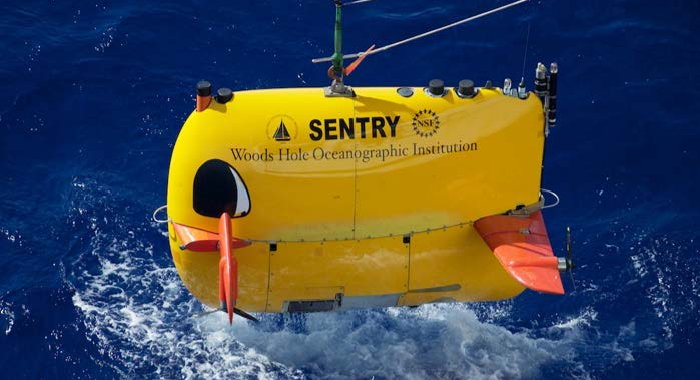
\includegraphics[width=\textwidth]{figures/sentry.pdf}
       \caption{Autonomous Underwater Vehicle, Sentry}
       \label{fig:sentry}
    \end{subfigure}
	\begin{subfigure}[b]{0.45\textwidth}
		\centering
		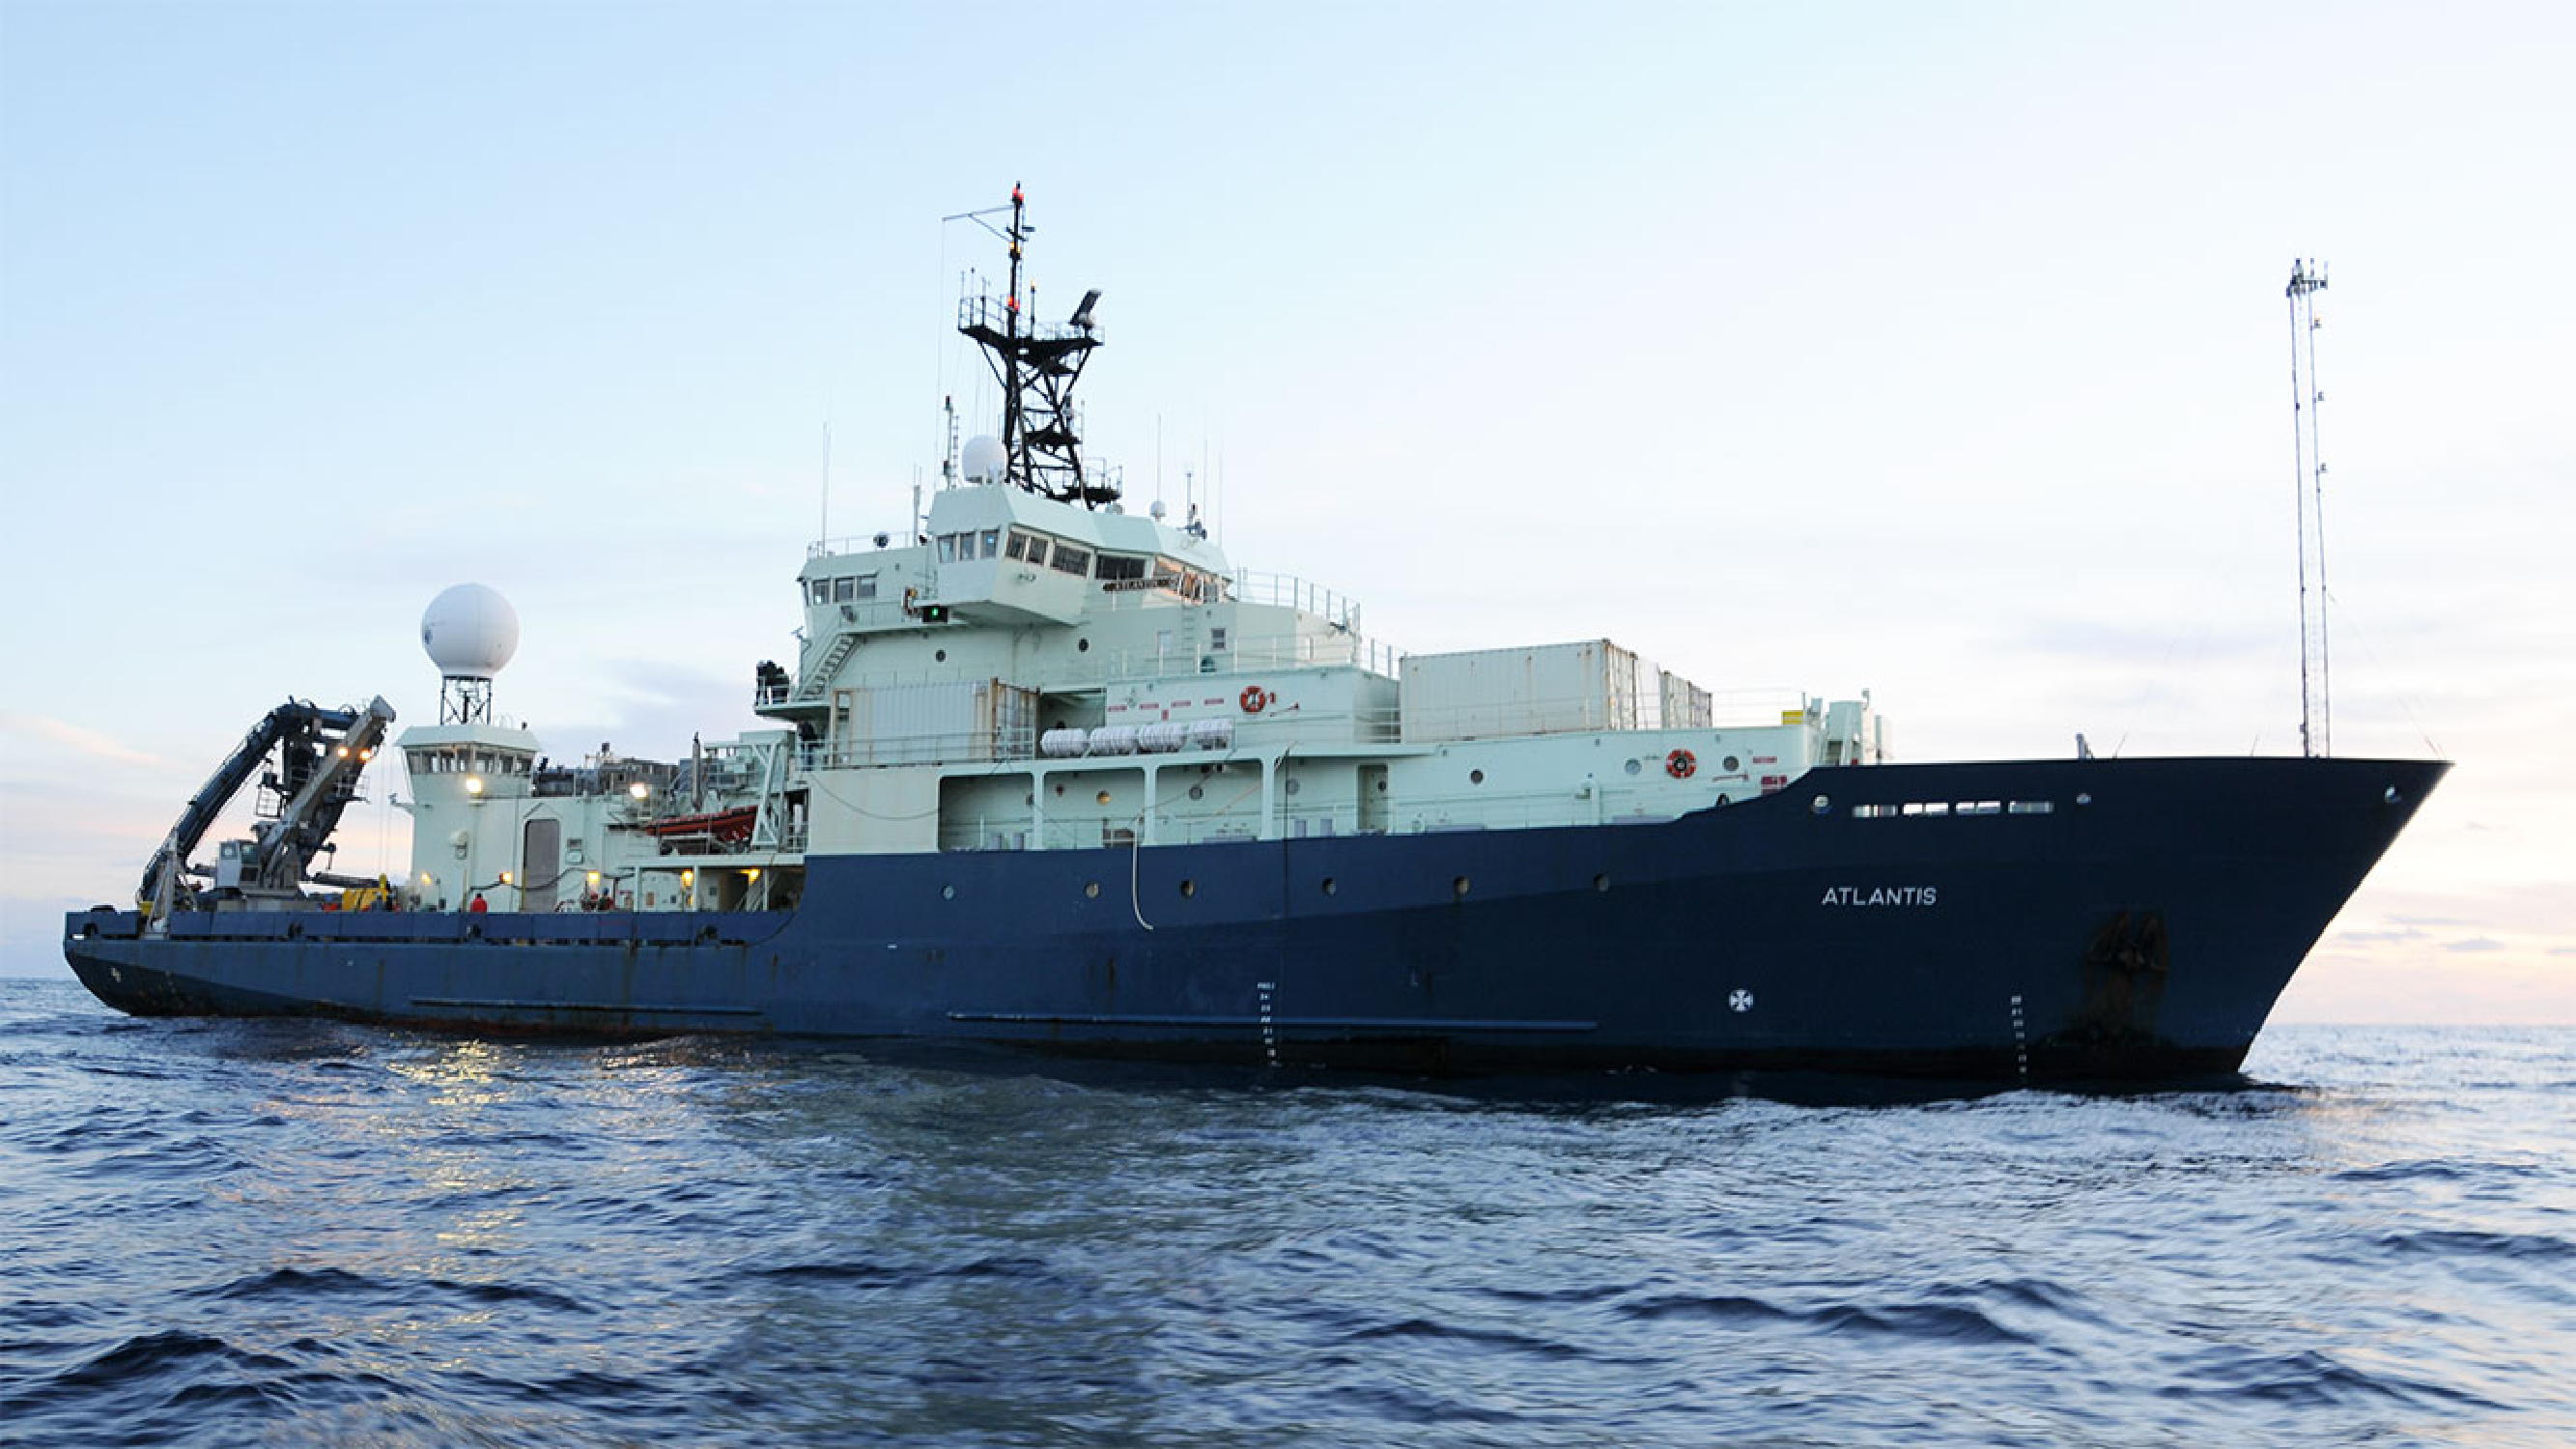
\includegraphics[width=0.975\textwidth]{figures/atlantis.pdf}
		\caption{Research Vessel, Atlantis}
		\label{fig:atlantis}
	\end{subfigure}
	\begin{subfigure}[b]{0.45\textwidth}
		\centering
	     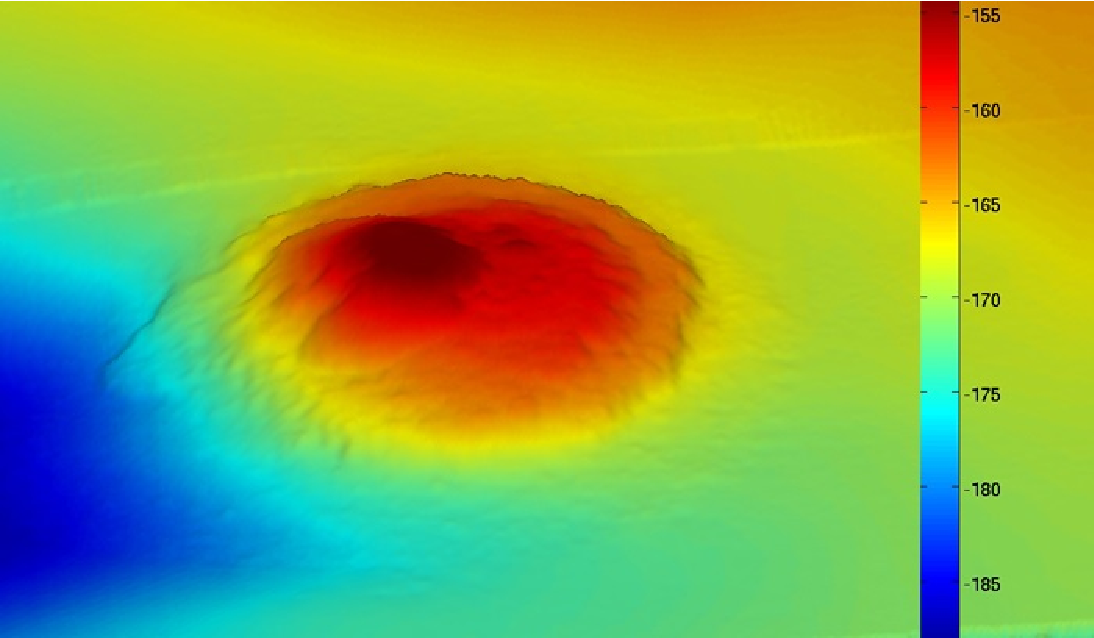
\includegraphics[width=0.97\textwidth]{figures/asphalt_domes.pdf}
	     \caption{Sonar data of an undersea asphalt mound collected by Sentry}
		 \label{fig:asphalt_domes}
	 \end{subfigure}
	 \begin{subfigure}[b]{0.45\textwidth}
		 \centering	    
	    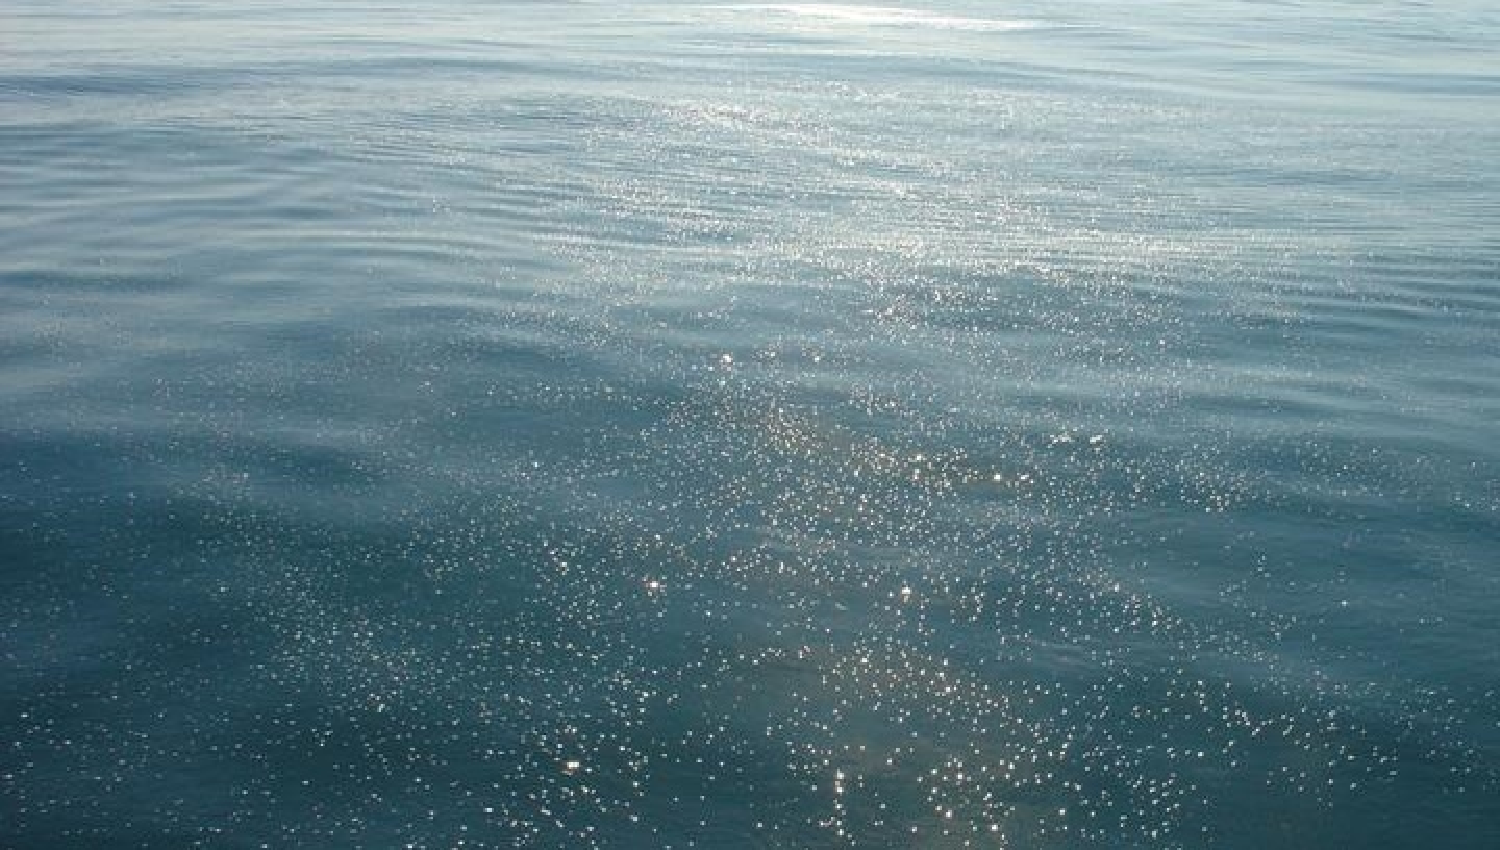
\includegraphics[width=\textwidth]{figures/methane_seeps.pdf}
	    \caption{An active methane seep in South Ellwood Oil Field (Photo by R K Nelson)}
	    \label{fig:methane_seeps}
	 \end{subfigure}
    \caption{Vehicles and survey targets of the example expedition (Courtesy WHOI)}
   	\label{fig:background_images}

\end{figure}


%Why do you add "controllable"?  The naming convention in the literature is to leave "controllable" as implied.  Such as
%(controllable) STN.  CTP, for Conditional Temporal Problem" is much simpler. 
%
%Are you recovering from a poor naming of CTP in the literature, where CTP includes uncontrolled durations?


We define the Controllable Conditional Temporal Problem (CCTP) formalism for
modeling Sentry's mission and the best plan for Rich, which includes: which
asphalt mounds site to survey, which methane seep site to scan, how much time to
spend at each site, and whether to extend the mission length. We start by
defining two variables for the choices he needs to make: AM (asphalt mounds
sites) and MS (methane seep sites). AM has two options in its domain: A (40) and
B (100). Each option is associated with a positive reward value that represents
Rich's preference towards it, the larger the better. The other variable MS for
methane seeps sites has three options: X (73), Y (80), and Z (47).


Next, we define twelve time points in the problem (Table \ref{table:events}): a
reference point in time ($S$) that represents the beginning of the trip at 11am;
a time point that indicates the end of the trip ($E$); and time points
representing the arrival and departure of each location (asphalt mounds sites A
and B, methane seep sites X, Y, and Z).

\begin{table}[h!]
	\centering
	\begin{tabular}{| m{3cm} m{1.5cm} | m{6cm} m{1.5cm} |}
		\hline
		\multicolumn{4}{|c|}{\textbf{Time Points}} \\
		\hline
		Mission starts & $S$ & asphalt
		mounds site A arrive/leave & $A_A$,$A_L$ \\
		Mission ends & $E$ & asphalt
		mounds site B arrive/leave & $B_A$,$B_L$ \\
		\hline
		\multicolumn{2}{|l}{methane seep site X arrive/leave} &
		\multicolumn{2}{c|}{$X_A$,$X_L$} \\
		\multicolumn{2}{|l}{methane seep site Y arrive/leave} &
		\multicolumn{2}{c|}{$Y_A$,$Y_L$} \\
		\multicolumn{2}{|l}{methane seep site Z arrive/leave} &
		\multicolumn{2}{c|}{$Z_A$,$Z_L$} \\
		\hline
	\end{tabular}
	\caption{Events in Sentry's mission CCTP}
	\label{table:events}
\end{table}



\begin{table}[h!]	
	\centering
	\begin{tabular}{| m{4.2cm} m{4.2cm} m{4.5cm}|}
		\hline
		\multicolumn{3}{|c|}{\textbf{Constraints (in minutes)}} \\
		\hline		
		$C_1$(R):$A_L$-$A_A\in[50,60]$ & $C_6$:$A_A$-$S\in[45,65]$ & $AM \leftarrow A$ \\ 
		$C_2$(R):$B_L$-$B_A\in[45,60]$ & $C_7$:$B_A$-$S\in[30,50]$ & $AM \leftarrow B$ \\ 
		$C_3$(R):$X_L$-$X_A\geq60$ & $C_8$:$E$-$X_L\in[28,35]$ & $MS \leftarrow X$ \\ 
		$C_4$(R):$Y_L$-$Y_A\geq65$ & $C_9$:$E$-$Y_L\in[30,32]$ & $MS \leftarrow Y$ \\ 
		$C_5$(R):$Z_L$-$Z_A\geq100$ & $C_{10}$:$E$-$Z_L\in[50,60]$ & $MS \leftarrow Z$ \\ 
		\hline
		\multicolumn{2}{|c}{$C_{11}$:$X_A$-$A_L\in[51,54]$} & $AM
			\leftarrow A$ and $MS \leftarrow X$ \\ 
		\multicolumn{2}{|c}{$C_{12}$:$Y_A$-$A_L\in[42,45]$} &$AM
			\leftarrow A$ and $MS \leftarrow Y$ \\ 
		\multicolumn{2}{|c}{$C_{13}$:$Z_A$-$A_L\in[30,55]$} & $AM
			\leftarrow A$ and $MS \leftarrow Z$ \\ 
		\multicolumn{2}{|c}{$C_{14}$:$X_A$-$B_L\in[22,24]$} & $AM
			\leftarrow B$ and $MS \leftarrow X$ \\ 
		\multicolumn{2}{|c}{$C_{15}$:$Y_A$-$B_L\in[21,25]$} & $AM
			\leftarrow B$ and $MS \leftarrow Y$ \\ 
		\multicolumn{2}{|c}{$C_{16}$:$Z_A$-$B_L\in[30,35]$} & $AM
			\leftarrow B$ and $MS \leftarrow Z$ \\ \hline
		
		\multicolumn{2}{|c}{$C_{17}$(R):$E$-$S\in[0,180]$} & 
		\\
		\hline
	\end{tabular}
	\caption{Conditional temporal constraints in the CCTP of Sentry's mission}
	\label{table:constraints}
\end{table}

\begin{figure}[h!]
	\centering
	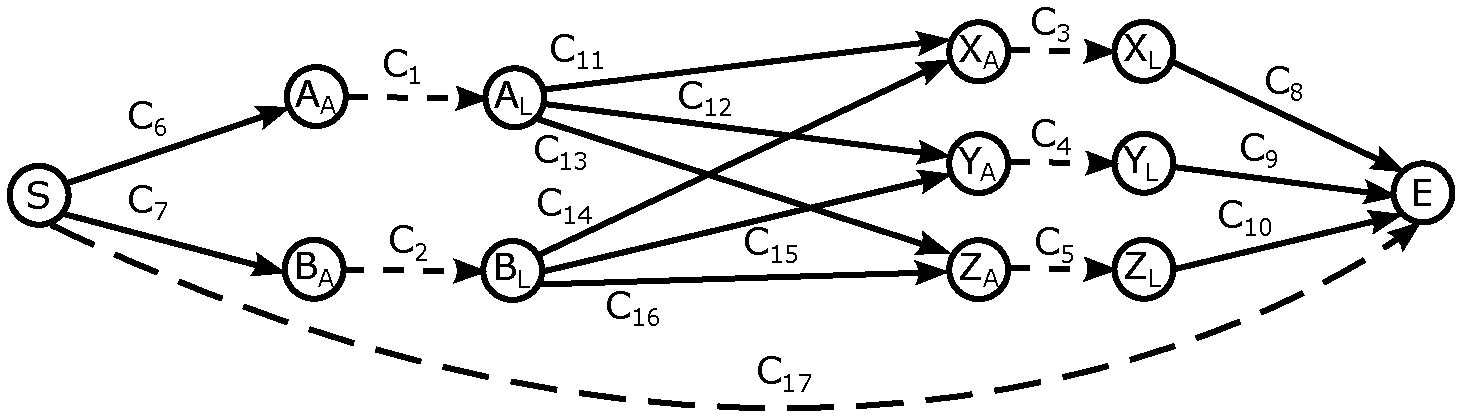
\includegraphics[width=0.80\textwidth]{figures/example_cctp.pdf}  
	\caption{A graphical representation of Rich's mission CCTP}
	\label{fig:example_cctp}
\end{figure}


%This is unclear.  Re-explain.
%
%First say that these constraints only hold for some choices, such as . . . .
%
%We represent this by saying that constraint * is ACTIVE only when the choice A = * is made, and indicate this by labeling the constraint * with *.  The constraint is called conditional, and the label is called the condition, or guard of the constraint. ....


Table \ref{table:constraints} shows all the conditional constraints in the CCTP
that encode the temporal relaxations between events. A subset of these constraints only hold for some choices, such as the duration of survey at site A ($C_1$) for assignment $AM\leftarrow A$. We represent this by saying that constraint $C_1$ is $ACTIVE$ only when the choice $AM\leftarrow A$ is made, and indicate this by labeling the constraint with $AM\leftarrow A$.  The label is called the guard of the conditional constraint. In this problem, constraints $C_1$ through
$C_5$ represent Rich's desired length of survey at
five locations. For example, $B_L$--$B_A\in [45,60]$ indicates that Rich would like
Sentry to spend between 45 and 60 minutes at asphalt mound site B. These constraints are labeled
by the assignments made to the decision variables: a constraint is activated
only if its label assignment is made. For example, $C_2$ will be considered only
if Rich chooses to visit site $B$, as shown in the right side of Table
\ref{table:constraints}. Constraints $C_6$ through $C_{16}$ are simple temporal
constraints that encode the traversal time required between locations. They are
conditioned on assignments made to either $AM$ or $MS$, or both ($C_{11}$
through $C_{16}$). Finally, $C_{17}$ constrains the duration of Sentry's mission
to three hours. Similar to previous temporal network representations in
literature, the CCTP can be visualized using a directed graph (Figure
\ref{fig:example_cctp}), in which nodes represent events and arcs represent temporal constraints.


Some of the constraints followed by a symbol `R' (also highlighted in dotted
arcs in the graph: $C_1$ through $C_5$ and $C_{17}$) are relaxable temporal
constraints. Their lower and/or upper bounds can be relaxed in order to restore
the consistency of the problem, if necessary. Each relaxable constraint comes
with one or two cost functions that describe Rich's preferences towards the
weakening for their upper and lower bounds. These functions map the relaxation
from $LB$ to $LB'$, or from $UB$ to $UB'$, to a positive cost value, as seen in
Figure \ref{fig:sample_pref1}. If the upper bound of $C_{17}$ is increased from
180 minutes to 200 minutes, meaning that Rich extends his mission by 20 minutes,
the cost will be 40. On the other hand, if he shortens the survey time by
reducing the lower bound of $C_3$ to 40, the cost would be 80. In this example,
we assume that all other relaxable constraints have linear cost functions with
gradient 1 for simplicity, but the approach is generalizable to arbitrary
monotonic functions (decreasing for lower bounds, and increasing for upper
bounds).


\begin{figure}[h!]
	\centering
	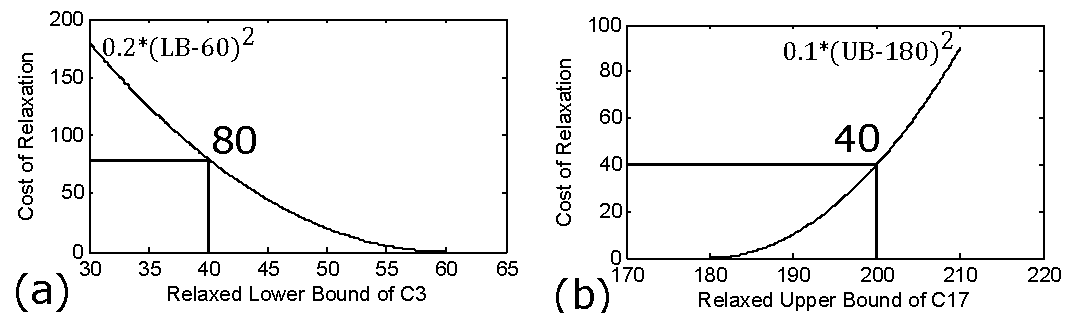
\includegraphics[width=0.80\textwidth]{figures/sample_pref.pdf}  
	\caption{Preference functions for $C_3$ and $C_{17}$}
	\label{fig:sample_pref1}
\end{figure}



\begin{table}[h!]
	\centering
	\begin{tabular}{| p{3cm} | p{1.8cm} | p{3cm} | p{1.8cm} | p{3cm} |}
		\hline
		\textbf{Relaxation 1} & & \textbf{Relaxation 2} & & \textbf{Relaxation 3} \\
		\hline
		$AM \leftarrow B$ &  \multirow{5}{*}{\parbox{2cm}{Rich told\\ system\\ \textbf{``Do not\\ relax $C_{17}$"}}}  & $AM \leftarrow B$ & \multirow{5}{*}{\parbox{2cm}{Rich told\\ system\\ \textbf{``$C_{2}$ is at\\ least 44"}}}  & $AM \leftarrow B$ \\
		$MS \leftarrow Y$ & & $MS \leftarrow X$ & & $MS \leftarrow Y$ \\
		$C_2$ to $\in[39,60]$ & & $C_3$ to $\geq57.5$ & & $C_4$ to $\geq55$ \\
		$C_{17}$ to $\in[0,185]$ & & $C_2$ to $\in[42.5,60]$ & & $C_2$ to $\in[44,60]$ \\
		Utility: 171.5 & & Utility: 169.25 & & Utility: 169 \\
		\hline
	\end{tabular}
	\caption{Three preferred relaxations to Rich's original CCTP}
	\label{table:relaxations}
\end{table}

%Your mixxing problem statement with algorithm, BCDRO, and system Uhura.
%
%don't do this.  This section is only about the problem statement, not about how Uhura interacts, or how BCDR behaves.  What you show here should relfect precisely the problem statement.  If you want to show how the problem statement is used within a scenario, thats good, but belongs in a separate section.

Before relaxing any constraints, there is no consistent solution to the problem.
The cause of failure is that three hours is not enough for Sentry to complete
both tasks: traversing to the nearest asphalt mounds and methane seep site
will consume at least 80 minutes, which brings the minimum trip duration to nearly 190
minutes. Therefore, one or more temporal constraints need to be relaxed. Table
\ref{table:relaxations} shows three consistent relaxations for the CCTP ranked
in best-first order. Relaxation 1, which is first presented to Rich, suggests
visiting site $B$ and $Y$. The survey time for $B$ should be reduced to 39
minutes and the mission should be extended by 5 minutes. The utility of the
relaxation is 171.5, which is computed by summing up the reward of two
assignments, $AM \leftarrow B$ and $MS \leftarrow Y$ , and subtracting the cost
of relaxing $C_2$ and $C_{17}$. If Rich changes his mind and decides not to
relax $C_{17}$, Relaxation 2 will be generated which incorporates this new
requirement. It takes Sentry to methane seeps site $X$, shortens the scan time
to 57.5 minutes and reduces the survey time at $B$ to 42.5 minutes. If Rich is still
unsatisfied and adds an additional requirement that survey time at the
asphalt mound site should be no less than 44 minutes, Relaxation 3 will be presented, which respects both newly added requirements.\\



%Introduce the section.  What is the ultimate goal?  Its about defining CCTPs.  Say so, and remind us what the essential features of a CCTP are.  
%
%Then say that you review the definition of the standard concept of CTP, as a stepping stone.  Explain why you do this, and explain the important difference.  Then dive into defining CTP.


\noindent\textbf{Definitions} \indent The example illustrates the
modeling of over-constrained temporal problems with the CCTPs, and demonstrates
the most significant advantage of continuous relaxation: it minimizes
perturbation to the original problem. Compared to discrete relaxations, which
may ask Rich to give up on the survey for asphalt mound sites or methane seeps,
continuous relaxations preserve more of the original problem while restoring
consistency. In this subsection, we formally define the Controllable Conditional
Temporal Problem formalism, explain its two essential features of relaxable
constraints and guarded elements, and present how it is different from other
temporal problem models in literature.


Temporal problems with choices can be modeled using Conditional Temporal
Problems (CTPs) \cite{Tsamardinos_CTP_2003}. We will start by reviewing the definition of this formalism as a stepping stone. CTP is a generalization of the
restricted problem class of Simple Temporal Problems \cite{Dechter_TCN_1991} by
adding uncontrollable outcomes of actions and by conditioning the occurrence of
events and simple temporal constraints on the outcomes of these choices.
Conditional Temporal Problems (CTPs) are capable of modeling conditional plans
and uncertainty during executions.


\begin{mydef}
	
	A CTP is a 6-tuple $\langle P,V,E,Q,L,OV\rangle $ where:
	
	\begin{itemize}

		\item $P$ is a set of Boolean atomic propositions.
		\item $V$ is a set of events, each with the domain of the Reals.
		\item $E$ is a set of simple temporal constraints that restricts the time points in V, and are of the form $l_{ij}\leq v_j-v_i\leq u_{ij},
		l_{ij},u_{ij}\in\mathcal{R}$.
		\item $Q$ is a set of literals of $P$.
		\item $L:V \rightarrow 2^Q$ is a function that attaches conjunctions of
		literals, $q_i\in Q$, to each event $v_i\in V$.
		\item $OV\subseteq V$ is a set of observation events that provides the truth
		value for $p_i\in P$ through function $O:P\rightarrow OV$.
		
	\end{itemize}
\end{mydef}


In a CTP, each event is associated with a conjunction of literals, called a
\textit{label}. If the label of an event is evaluated to be true, the event is
said to be activated and needs to be scheduled. Otherwise, the event is said to
be inactive and does not need to be scheduled. All temporal constraints
associated with an inactive event do not need to be satisfied.


The solution to a CTP is a dynamic schedule that is able to react to
observations in real time, such that all temporal constraints will be satisfied
no matter how the uncontrollable outcomes turn out. Conditional
Temporal Problems with Preferences \cite{Falda07dynamicconsistency}
extend CTPs by allowing fuzzy temporal constraints and fuzzy atomic
propositions. It allows the user to specify preferences over the execution time
of each event $v_i\in V$, and compare two schedules $T_1$ and $T_2$ using a
preference function that maps a schedule to a utility value $f:T\rightarrow
\mathcal{R}^{+}$ \cite{Khatib01temporalconstraint}.


The relaxation problems presented here, called Controllable Conditional Temporal Problems
(CCTPs), are closely related to CTPs; however, there are two important
differences. 


First, CCTPs assume that all real-valued variables (events) and finite-domain
variables (choices) are controllable, meaning that they are under the control of the agent. Consequently, to determine the consistency
of a CCTP, it is sufficient to have a single interpretation that satisfies all
activated constraints, where an interpretation is a set of assignments to all discrete and
continuous variables.


%Shouldn't this have been introduced in your informal example?
%
%Do you use the correct terminology for conditional CSPs?  For example, these are called activation constraints.  Alterantively, you can do what I do, and use the term "guard" to refer to the activation of either variables or constraints.  This is probably simpler.
%
%Again, its okay to change terminology.  Conditional CSPs were first called dynamic CSPs.  But only change for good reason.

Second, CCTP extends the domains of discrete variables from binary to finite
domain. In addition, it allows the discrete variables to be guarded by a set of assignments, which are called the guard assignments for the variable.


%Talk about related work AFTER you define CCTP.  You can't relate to CCTP when you haven't defined it first.
%
%Its much harder for the reader to follow when you interpose all the related work in the middle of your definition.  This requires the reader to go breadth first, rather thqn depth first, and leave lots of things on their mental stack.  Thats tiring.


\begin{mydef}
	A CCTP is a 9-tuple $\langle P, Q, V, E, RE, L_e, L_p, f_p, f_e\rangle$, where:
	\begin{itemize}
		
		\item $P$ is a set of controllable guarded finite domain variables;
		\item $Q$ is the collection of assignments to $P$;
		\item $V$ is a set of events representing designated time points;
		\item $E$ is a set of guarded temporal constraints between pairs of events $v_i\in V$;
		\item $RE \subseteq E$ is a set of relaxable constraints whose temporal bounds can be
		relaxed;
		\item $L_e:E \rightarrow 2^Q$ is a function that attaches conjunctions of
		assignments in $Q$, $q_i\in Q$, to some temporal constraint $e_i\in E$;
		\item $L_p:P \rightarrow 2^Q$ is a function that attaches conjunctions of
		assignments in $Q$, $q_i\in Q$, to some discrete variable $p_i\in P$;
		\item $f_p:Q\rightarrow \mathcal{R}^{+}$ is a function that maps each
		assignment to every controllable discrete variable, $q_i\in Q$, to a
		positive \textbf{reward} value;
		\item $f_e:(e_i,e_i^{\prime})\rightarrow \mathcal{R}^{+}$ is a function
		that maps the relaxation to one relaxable temporal constraint $e_i\in RE$,
		from
		$e_i$ to $e_i^{\prime}$, to a positive \textbf{cost} value.
	\end{itemize}
\end{mydef}

%After the definition
%
%1) give me your grounded example encoded as a CCTP, so that I can test my understanding.  Putting this in a table might help.
%
%2) discuss the interesting features of this definition, as you do here.
%
%3) then describe how parts of the definition relate to other definitions in the literature.
%
%You do a nice job of relating, but you mix 2) and 3).  I think its simple if you do 2) first, then 3).

Here we refer to the deep-sea exploration scenario as a grounded
example for the definition. In the CCTP model of the scenario, $P$ contains two
finite domain variables $AM$ and $MS$. Their domain values $Q$ contains two
sets: \{$A,B$\} for $AM$ and \{$X,Y,Z$\} for $MS$. The set $V$ of the CCTP
contains all events in Table \ref{table:events}, while the set $E$ contains all
constraints in Table \ref{table:constraints}. The relaxable constraints, $RE$,
consists of $C_1$ through $C_5$ and $C_{17}$. Labeling function $L_e$ attaches
assignments of $AM$ and $MS$ to guarded constraints in $E$, which are
constraints $C_1$ through $C_{16}$ in this example. Finally, the assignment reward
function, $f_p$, is defined over the five variable assignments and associates
them with positive real values: $AM\leftarrow A$ (40), $AM\leftarrow B$ (100),
$MS\leftarrow X$ (73), $MS\leftarrow Y$ (80) and $MS\leftarrow Z$ (47). While
the relaxation cost function, $f_e$, is defined over the six constraints in
$RE$, as shown in Figure \ref{fig:sample_pref1}.

%Why this difference?
%Why is this important?

To allow the continuous relaxation for an over-constrained temporal problem, we
include relaxable temporal constraints in the definition of CCTP ($RE$), similar
to the soft constraints in a Simple Temporal Problem with Preferences
\cite{Rossi_STPP_2002}. We do not use a disjunctive set of temporal bounds for
soft constraints. Instead, the constraint is soft in that its lower or upper
bounds can be relaxed \textbf{continuously} at the price of increasing cost. The
cost is defined over the degree of relaxation made to the lower and upper
bounds. Continuous relaxation provides greater flexibility in resolving
over-constrained temporal problems: it does not limit our options to the
predefined alternative temporal bounds, and allows us to weaken the constraint
to the minimum extent necessary.


In the CCTP formulation, there is one reward function, $f_p$, and one cost
function $f_e$. $f_p$ is defined over the assignments to controllable discrete
variables $q_i\in Q$. Each assignment is mapped to a positive reward value, such
as $MS \leftarrow X:73$. The larger the number is, the more preferred the choice
will be. $f_e$ is defined over relaxable constraints. The cost of relaxing an
upper bound constraint $E_{ij}:v_j-v_i\leq u_{ij}$ from $u_{ij}$ to
$u_{ij}^{\prime}$ is $f_{eij}(u_{ij}^{\prime}-u_{ij} )$. Figure
\ref{fig:sample_pref1}b shows an example function defined over
$u_{ij}^{\prime}-u_{ij}$.


%Why?  You need to justify each new feature of your definition.
%The motivation for this assumption is that ...

The cost function for temporal constraints that restrict the lower bounds
between two events is $f_{eij}(l_{ij}-l_{ij}^{\prime})$. This is illustrated in
Figure \ref{fig:sample_pref1}a. We assume that the user always prefers smaller
relaxations: the values in the original constraints are equally and maximally
preferred, and the preferences decreases as one moves away from the original
bounds. The motivation of this assumption is that people generally prefer to
minimize the perturbations to the original requirements, and penalize larger
deviations from them. Therefore, all $f_e$ functions must be monotonically
increasing, and equal to 0 when there is no relaxation. $f_e$ can be viewed as a
semi-convex \cite{Khatib01temporalconstraint} function with a segment of zero
cost when there is no relaxation. This assumption simplifies our relaxation
process, as the tightest relaxation will always result in the lowest cost. For
relaxable simple temporal constraints, two separate cost functions are required
for the lower and upper bounds.


\begin{mydef}
	A solution to a CCTP is a pair $\langle A,R_e\rangle$ such that all activated constraints are temporally consistent, where:
	\begin{itemize}		
		\item $A$ is a set of assignments, A $\subseteq$ Q, that leaves no variable unassigned;
		\item $R_e$ is a set of temporal relaxations for some constraints in $RE$.
	\end{itemize}
\end{mydef}

%Indicate that this is a subordinate definition, by saying
%
%":where a temporal relaxation is ..."
%
%Why say continuous temporal relaxation, here, and temporal relaxation in the line above?  The difference is confusing?

where a temporal relaxation is defined as a tuple, $\langle e,r_L,r_U\rangle$, as the following:

\begin{itemize}		
	\item $e$ is a constraint in $RE$;
	
%	Define "weakened lower/up per bound".
	
	\item $r_L$ is a weakened lower bound for $e$ and $r_L\leq e_{lowerbound}$;
	\item $r_U$ is a weakened upper bound for $e$ and $r_L\geq e_{upperbound}$.
\end{itemize}



% Dont just assert.  Justify why this is reasonable.
%Give me example solutions for your running example.  Show me how the utility was computed.

The utility of a solution is computed by subtracting the relaxation cost from
the assignment reward: $\sum_{p_i}f_{p_i}(p_i\leftarrow
value_i)-\sum_{e_i}f_{e_i}(e_i\rightarrow e_i^{\prime})$.  For example, Solution
1 in Table \ref{table:relaxations} consists of two assignments and two
relaxations: assignment $AM\leftarrow B$ and $MS\leftarrow Y$ have reward of 100
and 80, while the cost of relaxing $C_2$ and $C_{17}$ are 6 and 2.5,
respectively. Hence the utility value of this solution is 171.5, which is
computed by summing up the rewards, and subtracting the cost of relaxing $C_4$
and $C_{17}$ from it. Given a CCTP, the most preferred relaxation to it is
the one with the highest utility value according to $f_p$ and $f_e$.


Compared to the Temporal Constraint Satisfaction Problems (TCSPs) and
Disjunctive Temporal Problems (DTPs) formulation
\cite{Dechter_TCN_1991,Stergiou_DTP_1998}, whose constraints are disjunctions of
possible simple temporal constraints, CCTP is often more compact for real-world
scenarios since it allows a sequence of temporal constraints to be conditioned
on choices. The Temporal Networks with Alternatives (TNA) formulation, introduced by \citeA{bartak2007temporal}, also address this issue by introducing the concepts
of \textit{parallel} and \textit{alternative} processes. However, due to its
nested network structure, it is often less efficient in encoding constraints
that are conditioned on assignments to two independent variables, such as the
traversals between asphalt mound and methane seep sites.


%Why did you rename, when they are in essence the same?
Note that CCTP is similar, though different in notation, to the Optimal
Conditional Simple Temporal Problem (OCSTP) formulation, which was introduced by
\citeA{bobby_2006}. OCSTP and CCTP are equally expressive
for consistency problems. OCSTP encodes temporal constraints as the domain
values of discrete variables, and its relaxations are represented by additional
domain values. This makes it difficult to encode the relaxable temporal
constraints using an OCSTP formulation. We chose CCTP for
relaxation problems because of its compact representation of constraint
relaxations: consistency can be restored by relaxing the lower or upper bounds
of relaxable temporal constraints.


%Why add "controllable".  Seems like unneeded adjectives.
\subsection{Controllable Conditional Temporal Problems with Uncertainty}

%Update your remaining definitions, based on the spirit of my comments for your first definition.
%
%Rethink naming convention.

Uncertainty is commonly encountered in temporal scheduling and planning
problems, and can often lead to over-constrained situations. In Rich's mission
described earlier, the traversal times between locations are often
non-deterministic. When applying the deterministic formulation to model such
problems, their relaxations may fail since they only satisfy a subset of the
possible outcomes for the uncertain durations. Hence, we introduced the
Controllable Conditional Temporal Problem with Uncertainty (CCTPU) formalism; an
extension to the CCTP formulation, for modeling relaxation problems with
uncertain duration. Their definitions differ only in the terms of constraints:
in addition to temporal constraints with controllable durations, a CCTPU may also
contain uncertain durations. This is similar to
to the generalization from STPPs to the Simple Temporal Problems with Preferences and Uncertainty (STPPUs) framework
\cite{rossi2006uncertainty}, which adds support for modeling contingent events and uncertain durations.


We use Rich's mission to illustrate the modeling of relaxation problems
with uncertainty duration. Table \ref{table:constraints} repeats all the
constraints for his mission. Note that Constraints $C_6$ through $C_{16}$ are
highlighted in bold: they are uncontrollable temporal durations and encode the
traversal times between locations. Their temporal bounds indicate the domain of
the random outcomes. The survey times remain deterministic as we can give a deadline for departure from each survey location. Similar to CCTP, CCTPU can also be visualized using a
node-arc graph, in which uncontrollable durations are represented by double arcs
(Figure \ref{fig:example_cctpu}).

\begin{table}[ht!]	
	\centering
	\begin{tabular}{| m{4.2cm} m{4.2cm} m{4.5cm}|}
		\hline
		\multicolumn{3}{|c|}{\textbf{Constraints and Uncertain Durations (in minutes)}} \\		
		\hline		
		$C_1(R)$:$A_L$-$A_A\in [50,60]$ & $\mathbf{C_6}$:$A_A$-$S\in[45,65]$ & $AM \leftarrow A$ \\ 
		$C_2(R)$:$B_L$-$B_A\in [45,60]$ & $\mathbf{C_7}$:$B_A$-$S\in[30,50]$ & $AM \leftarrow B$ \\ 
		$C_3(R)$:$X_L$-$X_A\geq60$ & $\mathbf{C_8}$:$E$-$X_L\in[28,35]$ & $MS \leftarrow X$ \\ 
		$C_4(R)$:$Y_L$-$Y_A\geq65$ & $\mathbf{C_9}$:$E$-$Y_L\in[30,32]$ & $MS \leftarrow Y$ \\ 
		$C_5(R)$:$Z_L$-$Z_A\geq100$ & $\mathbf{C_{10}}$:$E$-$Z_L\in[50,60]$ & $MS \leftarrow Z$ \\ 
		\hline
		\multicolumn{2}{|c}{$\mathbf{C_{11}}$:$X_A$-$A_L\in[51,54]$} & $AM \leftarrow A$ and $MS \leftarrow X$ \\ 
		\multicolumn{2}{|c}{$\mathbf{C_{12}}$:$Y_A$-$A_L\in[42,45]$} & $AM \leftarrow A$ and $MS \leftarrow Y$ \\ 
		\multicolumn{2}{|c}{$\mathbf{C_{13}}$:$Z_A$-$A_L\in[30,55]$} & $AM \leftarrow A$ and $MS \leftarrow Z$ \\ 
		\multicolumn{2}{|c}{$\mathbf{C_{14}}$:$X_A$-$B_L\in[22,24]$} & $AM \leftarrow B$ and $MS \leftarrow X$ \\ 
		\multicolumn{2}{|c}{$\mathbf{C_{15}}$:$Y_A$-$B_L\in[21,25]$} & $AM \leftarrow B$ and $MS \leftarrow Y$ \\ 
		\multicolumn{2}{|c}{$\mathbf{C_{16}}$:$Z_A$-$B_L\in[30,35]$} & $AM \leftarrow B$ and $MS \leftarrow Z$ \\ \hline
		\multicolumn{2}{|c}{$C_{17}(R)$:$E$-$S\in[0,180]$} & \\
		\hline
	\end{tabular}
	\caption{Temporal constraints and uncertain duration in Rich's mission CCTPU}
	\label{table:stnu_constraints}
\end{table}

\begin{figure}[h!]
	\centering
	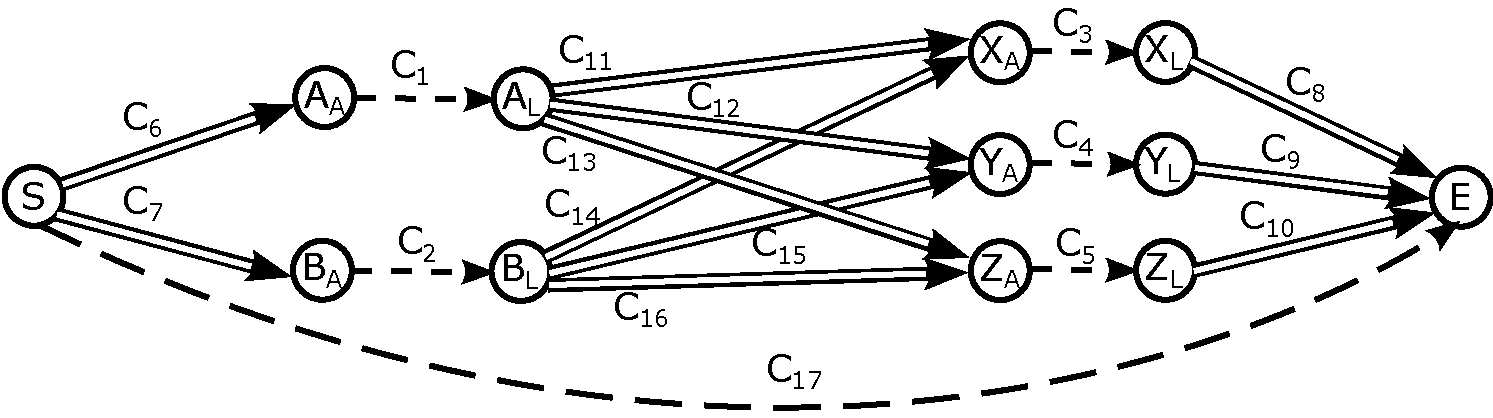
\includegraphics[width=0.80\textwidth]{figures/example_cctpu.pdf}  
	\caption{A graphical representation of Rich's mission CCTPU}
	\label{fig:example_cctpu}
\end{figure}


Similar to the earlier example, without any relaxations, there is no solution
that can satisfy all of the requirements in Rich's mission. If we use the CCTP
formalism to model this over-constrained problem, one solution would be to visit
site B and X while extending the mission by 5 minutes (Figure
\ref{fig:ConsistentSolution}). However, it does not account for the
uncontrollable traversal times: the solution is very likely to fail during the
mission, since it has no margin to absorb any delay in the traversal between
locations. Next, we present two solutions generated for the CCTPU model, which
are based on two execution strategies that take the uncertainty into
consideration. The first strategy, called \textit{Strong Controllability}, comes
up with a schedule of activities before starting the plan, which ensures success
for all uncontrollable durations. The second execution strategy, called
\textit{Dynamic Controllability}, instead observes these uncertain outcomes
along the way, and makes \textit{more informed} decisions about scheduling each
activity.


\begin{figure}[!ht]
	\centering
	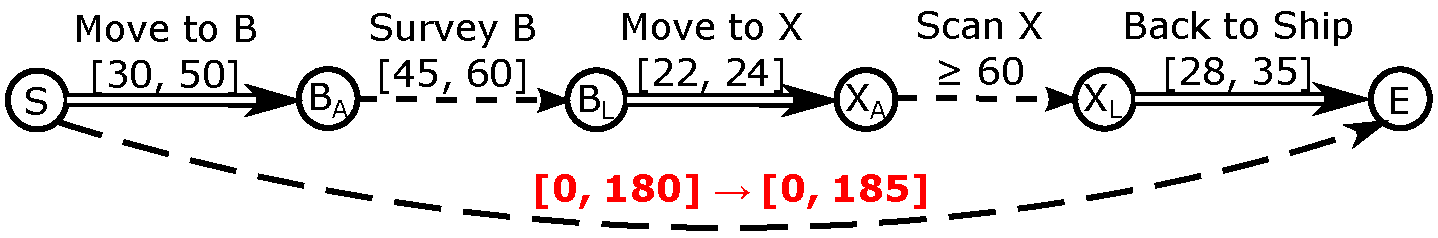
\includegraphics[width=0.8\textwidth]{figures/solution_consistent.pdf} 
	\caption{Consistent relaxation for Rich's mission}
	\label{fig:ConsistentSolution}
\end{figure}

\begin{figure}[ht!]
	\centering
	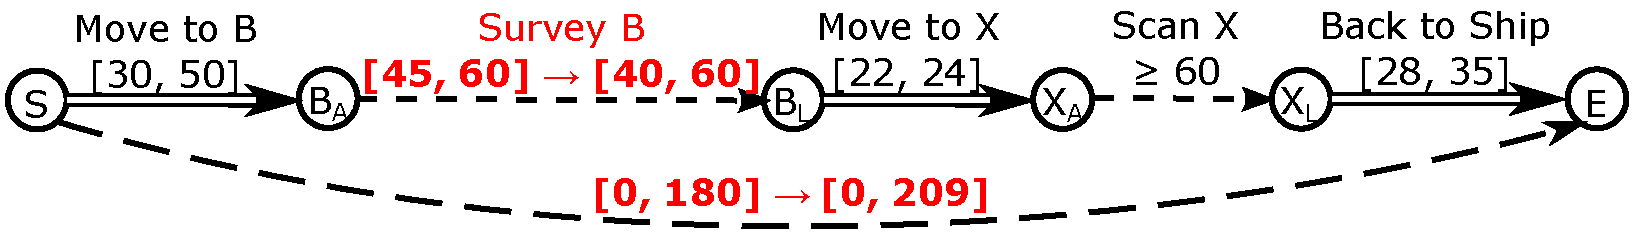
\includegraphics[width=0.9\textwidth]{figures/solution_sc.pdf}
	\caption{Strongly controllable relaxation for Rich's mission}
	\label{fig:SCSolution}
\end{figure}

The second solution is computed based on strong controllability (Figure
\ref{fig:SCSolution}). It extends the mission time to 209 minutes, and decreases
the lower bound of the survey time at $B$ to account for the uncertainty in
the traversal between the ship and site $B$. This solution has a utility of
83.9, and enables a schedule that satisfies Rich's requirements while being robust to
the uncertain durations.

\begin{figure}[ht!]
	\centering
	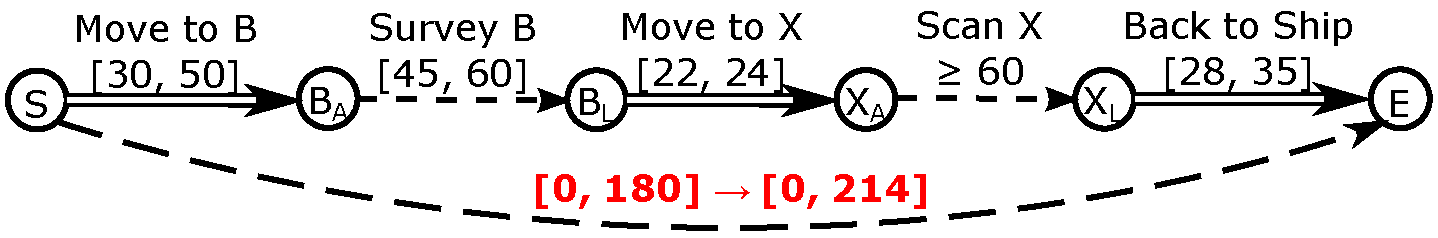
\includegraphics[width=0.8\textwidth]{figures/solution_dc.pdf} 
	\caption{Dynamically controllable relaxation for Rich's mission}
	\label{fig:DCSolution}
\end{figure}

The third and final solution is computed based on dynamic controllability
(Figure \ref{fig:DCSolution}). Unlike the strong controllability solution, it
does not need to decrease the lower bound of survey time at $B$ to account for
the uncertain traversal times, and hence is less conservative than the second
solution, while still being safe. The solution has a higher utility of 57.4, and
enables a dynamic schedule on the fly instead of a static schedule beforehand:
the times of leaving site $B$ and $X$ will depend on the actual traversal times.


\subsubsection{Definitions}

Simple Temporal Networks with Uncertainty (STNUs)
\cite<STNUs,>{Vidal99handlingcontingency} have been widely used to model temporal
problems with uncertain durations. They are extension to STNs by adding a new
class of constraint: \textit{uncertain duration}. The duration is defined by a
random variable between its lower and upper bounds and cannot be freely
assigned. Formally, this structure is defined as the following:

\begin{mydef}
	A STNU $N = \langle V_a, V_r, E_f, E_u\rangle$, extends the STN definition with new types of events and constraints
associated with the uncertain duration:
	
	\begin{itemize}
		\item activated events $v_i \in V_a$, whose times are assigned by the agent;
		\item received events $r_i \in V_r$, whose times are assigned by external
world;
		\item free constraints $e_i \in E_f$, which are of type $v_x - v_y \in
[l_{xy},b_{xy}]$ where $v_x, v_y$ are events. 
		\item uncertain durations $u_{xy} \in E_u$, where $u_{xy} \in [l_{xy},b_{xy}]$ describes the difference in time
		 between one received event $r_y\in V_r$ and one activated event $v_x\in V_a$, such that $(r_y - v_x) = u_{xy}$; or between two received events $r_y, r_x\in V_r$, such that $(r_y - r_x) = u_{xy}$. 
		 Uncertain durations are not assigned by the agent, and can take any value in the bounded interval. 
	\end{itemize}
	
\end{mydef}

The STNU extends the STN representation with uncertainty. Note that the uncertainty representation is not probabilistic: 
the uncertain durations are not associated with probability distributions. Thus, we can not reason over the likelihood of 
outcomes for the uncertain durations. We must instead guarantee constraint satisfaction given any outcome for the uncertain
duration within the interval. 

The solution to a STNU is an execution strategy that satisfies all constraints
regardless of the outcomes of uncertain duration. The existence of such a
strategy is characterized by the controllability, instead of consistency, of the
STNU. There are three types of controllability \cite{Vidal99handlingcontingency}: \textit{Strong},
\textit{Dynamic}, and \textit{Weak}. Each type has a different assumption about
the time when the outcomes of uncertain duration become available. In this
paper, we focus on the first two types, strong and dynamic controllability,
which assume that no outcome is known prior to the execution. Strong
controllability requires a predetermined schedule which satisfies all
constraints regardless of the outcomes of the uncertain durations, whereas
dynamic controllability requires a policy for scheduling as observations of
uncertain durations become available. Intuitively, dynamic controllability is
more flexible as it makes use of information gained during execution.

\begin{mydef}

	A Simple Temporal Problem with Uncertainty, STPU, is a problem formulation
using the STNU representation.
	\begin{itemize}
	\item Given a STNU $N = \langle V_a, V_r, E_f, E_u\rangle$, find an execution
policy to  events in $V_a$ such that all constraints in $E_f$ are satisfied
regardless of the outcomes of durations in $E_u$.
	\end{itemize}
	
\end{mydef}

The STPU formalism has been extended with disjunctions and conditional
constraints to handle more real-world scheduling and planning problems. \citeA{Venable05disjunctivetemporal} and \citeA{Peintner_07} introduced the \textit{Disjunctive
	Temporal Problem with Uncertainty} (DTPU) formalism to permit
non-convex and non-binary constraints. DTPU can be viewed as an extension to the
deterministic Disjunctive Temporal Problem
formalism \cite{Stergiou98backtrackingalgorithms} with uncertain durations. It
allows the expression of disjunctive constraints, and enables the agent to
choose between alternatives. \citeA{Hunsberger12} introduced the Conditional Temporal Problems with Uncertainty (CTPUs) formalism to model problems with both uncontrollable duration and observations. We introduce CCTPU formalism to permit the description of more general scheduling and relaxation problems for scenarios with uncertain durations. It is equally expressive as DTPUs and allows more compact encodings of conditional decision variables and constraints. On the other hand, we are only concerned with controllable decision variables. This makes CCTPUs strictly simpler to solve compared to CTPUs, in that those tasks may require the enumeration of all scenarios that are dependent on uncontrollable variables.

Formally, the CCTPU formulation extends the CCTP definition with three additional elements.

\begin{mydef}
\label{def:CCTPU}
	A CCTPU contains all elements in a CCTP, plus $V_r$, $E_u$ and $RE_u$, where:
	
	\begin{itemize}
		\item $V_r\subseteq V$ is a set of received events. $V\backslash V_r$ is the
set of all activated events; 
		\item $E_u\subseteq E$ is a set of guarded uncertain duration between pairs of
activated and received events. The temporal bounds of these duration indicate the domain of possible values of the random outcomes. $E\backslash E_u$ is the set of all free constraints;
		\item $RE_u\subseteq E_u$ is a set of relaxable uncertain durations whose
		bounds can be tightened, and $RE_u\subseteq RE$.
	\end{itemize}
	
	The cost function is generalized to include both free constraints and uncertain
duration: $f_e:(e_i,e_i^{\prime})\rightarrow \mathcal{R}^{+}$ is a
	function that maps the following to a \textbf{non-negative cost}.
	\begin{itemize}
		\item the \textbf{relaxation} of a free constraint, $e_i\rightarrow
		e'_i,e_i\in RE\backslash RE_u$;
		\item or the \textbf{tightening} of an uncertain duration, $e_i\rightarrow
		e'_i,e_i\in RE_u$;
	\end{itemize}
	
\end{mydef}

As can be seen in the definition, we also generalize the concept of relaxations to include uncertain durations. To resolve a conflict by relaxing free constraints, we will either increase its upper bound or reduce its lower bound. On the other hand, we shrink the uncertainty for uncertain duration in a conflict: we may resolve the
conflict by increasing the lower bound and/or decreasing the upper bound of its
uncertain duration. Usually, uncertain duration is used to reserve some
flexibility for the agents or the environment in executing their tasks. A
tighter duration means less flexibility for them, but also imposes less
restriction on the solution to the temporal problem. We will give more insights
into the relation between uncertain durations and conflict resolutions in the
approach section. 


Similar to CCTP, the solution to a CCTPU is defined as a 3-tuple $\langle A,R_e,R_u\rangle$, where:
\begin{itemize}
	\item $A$ is a complete set of assignments to variables in $P$ that leaves
	no variable unassigned.
	\item $R_e$ is a set of relaxations for some free constraints
	in $RE\backslash RE_u$.
	\item $R_u$ is a set of tightenings for some uncertain durations in $RE_u$.
\end{itemize}

A feasible solution to a CCTPU provides a grounded and controllable STPU. We
separate the solutions into two categories: \textit{strongly controllable} and
\textit{dynamically controllable}. This is based on the type of execution
strategies a solution can enable.

\begin{itemize}
	
	\item A strongly controllable solution makes the resulting STPU strongly controllable. That is, the relaxation enables an execution strategy with a firm schedule for all events.  
	
	\item A dynamically controllable solution makes the resulting STPU dynamically
	controllable, for which a dynamic execution strategy that reacts in real time to observations of uncertain duration and meets all constraints can be derived. 
	
\end{itemize}

Note that a strongly controllable solution is also a dynamically controllable
solution, since strong controllability is more restrictive than dynamic
controllability. Due to the flexibility of dynamic controllability, there is usually a greater solution space to explore for this type of problem. 




\subsection{Conditional Probabilistic Temporal Problems with Chance-constraints}

In many situations, modeling the uncertainty in temporal duration with a
set-bounded representation is overly conservative, resulting in a loss of
schedule utility. Chance-constrained formalisms, such as chance-constrained
probabilistic Simple Temporal Problems (cc-pSTPs), address over-conservatism by
imposing bounds on risk, while maximizing utility subject to these risk bounds.
On the other hand, when we are dealing with probabilistic uncertain duration,
the relaxation problem becomes more challenging, since we are making trade-offs
between not only timing requirements, but also risk taken. In the rest of this
section, we present an extended formalism to CCTPs, the chance-constrained
probabilistic Controllable Conditional Temporal Problems (cc-pCCTPs) for modeling
relaxation problems with chance constraints. 

We again use Rich's mission as an example to illustrate the modeling. To
simplify the example, we remove the asphalt mound site survey, leave only the methane seeps sites to visit, and make the traversal duration controllable. The
periodic methane seeps at X is likely to occur at around 1:00PM, following a normal distribution with
a standard deviation of 30 minutes. The seeps at Y will occur at around
1:30PM and follows a normal distribution with a standard deviation of 50
minutes. As described before, Sentry leaves the ship at 11:00AM, and needs to
arrive at the site before the start of the methane seeps. In addition, at least 30
minutes is required for traversing to the site, and 45 minutes for scanning. As
before, Rich wants the mission to complete in 3 hours, with less than 5\% risk
of violating \textbf{any} constraint, such as returning late or missing the event. We
can capture this problem using a cc-pCCTP (Figure \ref{fig:sample_ccpctp}).

\begin{table}[ht!]	
	\centering
	\caption{Temporal constraints and uncertain duration in Rich's mission cc-pSTP}
	\begin{tabular}{| m{1.5cm} m{4.5cm}  m{1.7cm} m{6.0cm}|}		
		\hline
		\multicolumn{4}{|c|}{\textbf{Constraints and Uncertain Durations (in minutes)}} \\		
		\hline		
		$C_{1}$ & $X_A$-$S > [45,+\infty]$ & $MS \leftarrow X$ & Traversal to methane seeps site X\\
		$C_{2}$ & $X_{sp}$-$X_A\in[0,+\infty]$ & $MS \leftarrow X$ & Wait for seeps at site X \\
		$C_{3}$(R) & $X_L$-$X_{sp}\in[50,60]$ & $MS \leftarrow X$ & Scanning at site X \\ 
		$C_{4}$ & $E$-$X_L\in[45,+\infty]$ & $MS \leftarrow X$ & Traversal from site X back to ship \\
		$\mathbf{C_{5}}$ & $X_{sp}$-$S$ = [$\mu=120,\sigma=30$] & $MS \leftarrow X$ & Seeps start time at X \\
		$C_{6}$ & $Y_A$-$S\in[30,+\infty]$ & $MS \leftarrow Y$ & Traversal to methane seeps site Y\\
		$C_{7}$ & $Y_{sp}$-$Y_A\in[0,+\infty]$ & $MS \leftarrow Y$ & Wait for seeps at site Y \\
		$C_{8}$(R) & $Y_L$-$Y_{sp}\in[45,60]$ & $MS \leftarrow Y$ & Scanning at site Y \\ 
		$C_{9}$ & $E$-$Y_L\in[30,+\infty]$ & $MS \leftarrow Y$ & Traversal from site Y back to ship \\
		$\mathbf{C_{10}}$ & $Y_{sp}$-$S$ = [$\mu=150,\sigma=50$] & $MS \leftarrow Y$ & Seeps start time at Y \\  
		$C_{11}$(R) & $E$-$S\in[0,180]$ & & Mission duration \\  
		\hline
	\end{tabular}
	\label{table:ccpctp_constraints}
\end{table}

\begin{figure}[htb]
	\centering
	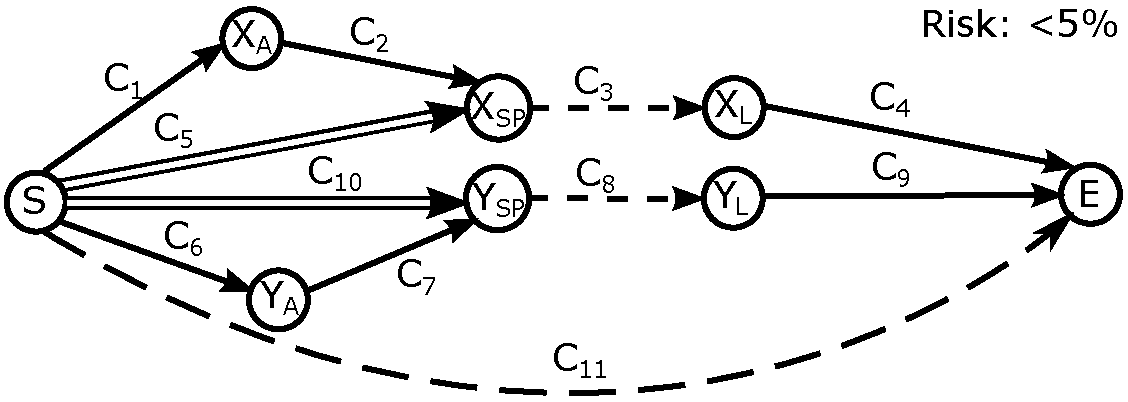
\includegraphics[width=0.7\textwidth]{figures/ccpstp_example.pdf}
	\caption{The cc-pCCTP model for Rich's mission}
	\label{fig:sample_ccpctp}
\end{figure}

After evaluating all the requirements, BCDR determines that no dynamic
execution policy exists that meets all requirements. It engages Rich and starts
presenting relaxations that can restore the feasibility of Rich's problem. The
first one asks Rich to \textbf{extend the mission} from 3 hours to 4 hours and 26
minutes, which is robust for surveying the methane seeps at site X if it occurs between 11:45AM
and 1:51PM (Figure \ref{fig:sample_ccpstp_sol1}). The probability of failure is determined by analyzing the assumptions on the uncertain duration: the probabilistic duration $C_5$ is turned into a set bounded one with bounds [45,171], and the network is checked to be dynamically controllable against all possible outcomes within the range.

\begin{figure}[htb]
	\centering
	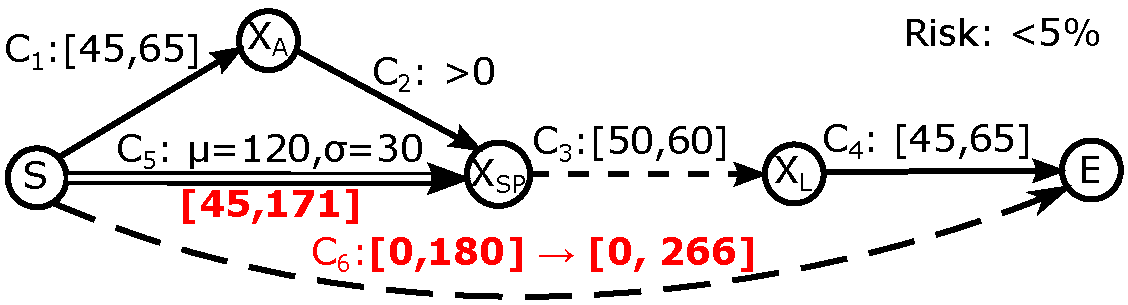
\includegraphics[width=0.65\textwidth]{figures/ccpstp_example_s1.pdf}
	\caption{First relaxation for Rich's mission}
	\label{fig:sample_ccpstp_sol1}
\end{figure}

However, Rich rejects the solution and tells BCDR that the mission duration can
be at most 4 hours, since the subsequent mission cannot be shortened by more
than an hour. BCDR incorporates this new requirement and generates another
relaxation, which requires Rich to accept an increased probability of failure, from 5\% to 20.85\%. This allows
the mission to be completed in 4 hours, but cannot account for methane seeps that
occurs after 1:25PM (Figure \ref{fig:sample_ccpstp_sol2}).

\begin{figure}[htb!]
	\centering
	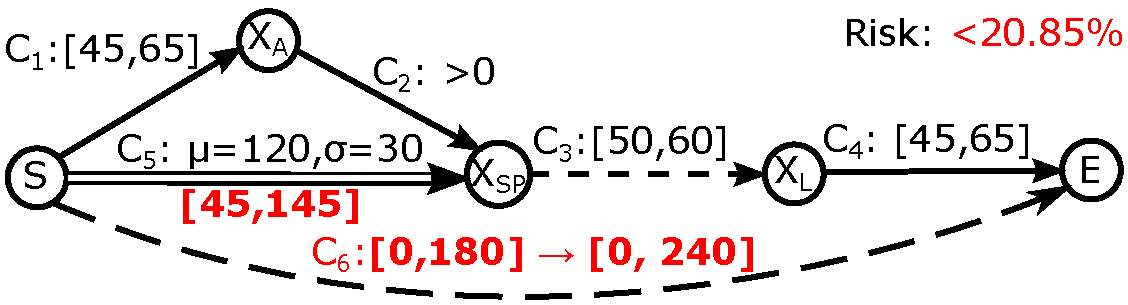
\includegraphics[width=0.65\textwidth]{figures/ccpstp_example_s2.pdf}
	\caption{Second relaxation for Rich's mission}
	\label{fig:sample_ccpstp_sol2}
\end{figure}

\begin{figure}[htb!]
	\centering
	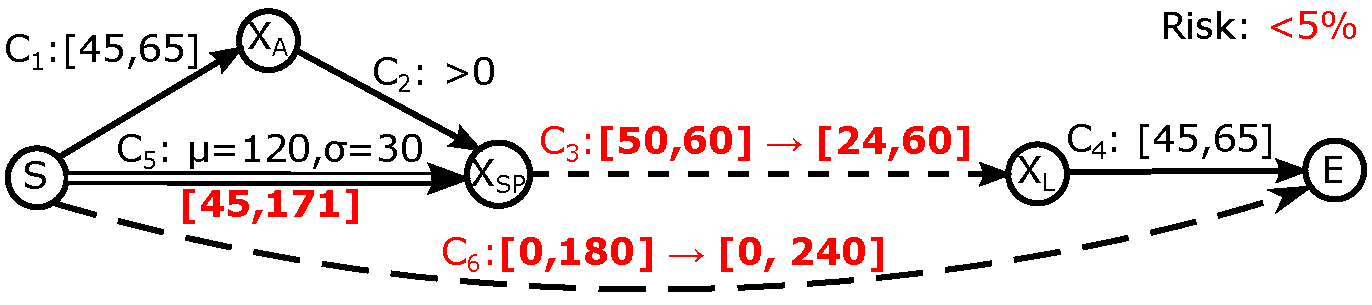
\includegraphics[width=0.75\textwidth]{figures/ccpstp_example_s3.pdf}
	\caption{Third relaxation for Rich's mission}
	\label{fig:sample_ccpstp_sol3}
\end{figure}



Rich rejects the solution again and tells BCDR that he cannot take more than
5\% risk. BCDR again incorporates this new constraint and generates the third
relaxation, which asks Rich to reduce the survey time
at site X to 24 minutes. This allows the mission to be
completed in 4 hours, while being robust to methane seeps that takes place between 11:45AM and
1:51PM (Figure \ref{fig:sample_ccpstp_sol3}).




\subsubsection{Definitions}

Similar to the STNU formalism, cc-pSTP is also an extension to the Simple
Temporal Problems (STPs) formulation. In addition to the simple temporal
constraints in STPs, it adds two new types of constraints to the problem:
probabilistic temporal constraints for modeling uncertain durations, and chance
constraints for specifying the acceptable level of risk. Compared to the
set-bounded uncertain durations used in STNUs, the
probabilistic representation of uncertain durations allows cc-pSTPs to more
accurately model uncertainty in real world activities. In addition, the chance
constraint supports a quantified bound on risk taken to be specified, which is
more flexible and intuitive than the criteria of controllability. It can be
viewed as a generalization of the notion of controllability: instead of a binary
outcome between 100\% guarantee of success or nothing, the users can ask for any
bound between [0,100\%] on the probability that a temporal network is
executable.

Chance-constraints have been studied in the operations research literature,
traditionally as probabilistic guarantees over satisfaction of  individual or
conjunctions of constraints \cite{kall1976chance}. In this work, we generalize
the definition of chance-constraints to include disjunctions over constraints as
well. It allows us to choose between multiple options to find one which meets
our safety requirements.

In the definition below, we use the standard definitions of random variables
from probability theory \cite{durrett2010probability}. Intuitively, when
describing outcomes of random variables, we can imagine sampling $\omega$ from a
sample space $\Omega$. The outcomes of random variables can be generated via
functions $\mathbf{f}(\omega)$. Further, we have a probability measure $P$,
which takes a subset $S\subseteq \Omega$ and gives the probability of samples
being in $S$.

A chance-constraint is rigorously defined as follows:

\begin{mydef}
Consider a constraint program with decision variables $\mathbf{x}$, and a set of random variables $\mathbf{f}(\omega)$ with probability measure $P$, sample space $\Omega$, and $\omega\in \Omega$. 

Let the set of constraints be defined over decision variables and random variables as 
\[C = \bigvee_{i\in I}\bigwedge_{j\in J_i} A_j(\mathbf{x},\mathbf{f}(\omega))\geq b_j \]
where each $A_j$ is a measurable function, $I$ can be thought of as a set of distinct scenarios, and $J_i$ can be thought of as a listing of the set of constraints required to hold in each scenario.

A \emph{chance-constraint} is a tuple $\langle C, \Delta\rangle$, requiring:
\begin{align}
P(C\text{ satisfied}) \equiv P\left(\left\{\omega\left|\bigvee_{i\in I}\bigwedge_{j\in J_i} A_j(\mathbf{x},\mathbf{f}(\omega))\geq b_j \right.\right\}\right) \geq \Delta
\end{align}
\label{def:chance-constraint}
\end{mydef}

As an example, consider a chance-constraint for Rich's mission in Figure \ref{fig:sample_ccpctp}. There are two distinct scenarios, in which sites X or Y are visited respectively. For the visit to site X, the constraints which must hold are $C_1$, $C_2$, $C_3$, $C_4$, and $C_11$, and for the visit to site Y, the constraints which must hold are $C_6$, $C_7$, $C_8$, $C_9$,and $C_11$. Note that, of the constraints, only $C_2$, $C_3$, $C_7$, and $C_8$ involve uncontrollable time points. Thus, we have our set of constraints $C$ in the chance constraint


\begin{align*}
C = \left((X_{sp}-X_A\geq 0) \land (X_L-X_{sp}\geq 50) \land (-X_L+X_{sp}\geq -60) \right) \lor \\
\left((Y_{sp}-Y_A\geq 0)\land(Y_L-Y_{sp}\geq 45)\land(-Y_L+Y_{sp}\geq -60)\right)
\end{align*}


While the definition here is presented for constraints systems in disjunctive normal form, this is a general representation with conversions via De Morgan's laws, and is sufficient for the chance-constrained problem definitions presented below.

The cc-pCCTP formalism extends CCTPU with probabilistic uncertain durations and chance
constraints. Here, we first repeat the definition of cc-pSTP, as presented by
\citeA{Fang_AAAI_2014}, for reference.


\begin{mydef}
	
	A cc-pSTP is a pair $\langle N^+,\Delta_t\rangle$, where:
	
	\begin{itemize}
		
		\item $N^+$ is a probabilistic Simple Temporal Network (pSTN), defined as a
		4-tuple $\langle V_a,V_r,E_f,E_d\rangle$, where:
		
		\begin{itemize}
			
			\item $V_a,V_r,E_f$ are defined as for STNU; and 
			
			\item $E_d$ is a set of probabilistic uncertain durations. Each $d_{xy}\in
			E_d, d_{xy}:\Omega\rightarrow\mathbb{R}$ is a random variable describing the difference $(y-x)$ between an activated 
			event $x\in V_a$ and a received event $y\in V_r$. 
			
		\end{itemize}
		
		\item $\langle E_f, 1 - \Delta_t\rangle$ is the chance constraint that sets the upper bound
		on the risk of failure, for the set of requirement constraints $E_f$ in $N^+$.
		
	\end{itemize}
	
	
\end{mydef}

In the cc-pSTP, the set of constraints is described by $E_f$, which are
difference constraints between elements in $V_r$ and $V_a$ to be satisfied,
given the outcomes of $E_d$. This corresponds to $C$ in Definition
\ref{def:chance-constraint}.

\begin{mydef}
	
	A cc-pSTP solution is a pair $\langle N_g,S_{x}\rangle$, where:
	
	\begin{itemize}
		
		\item $N_g$ is a grounded STNU of the cc-pSTP. It replaces all probabilistic
		durations in the cc-pSTP with set-bounded uncertain durations, which specify
		the allocated risk over them: the lower and upper bounds allocated for each
		probabilistic duration indicate the range of outcomes covered. The total
		probability of uncovered outcomes across all probabilistic durations must be
		smaller than the chance constraint.
		
		\item $S_x$ is an execution strategy for $N_g$. It covers all controllable
		events in the cc-pSTP, and is controllable with respect to $N_g$. 
		
	\end{itemize}
	
\end{mydef}


Given a cc-pSTP, $A$, if we execute the
controllable events using $S_x$ in its solution, the chance of violating any
temporal constraints in $A$ is guaranteed to be less than $\Delta_t$. The policy
$S_x$ could be a static schedule (with a strongly controllable $N_g$), or a
dynamic execution policy (with a dynamically controllable $N_g$). If a cc-pSTP
is over-constrained, no solution exists that can meet all temporal constraints
within the risk bound. In other words, there is no $N_g$ that is
controllable and takes less risk than the chance constraint. This occurs when
the user specifications are too restrictive, for example when the desired time
bounds are too tight, or when the user is overly cautious in setting the chance
constraint. These problems can be resolved through temporal or chance constraint
relaxations: they are trade-offs between
weakening over chance and temporal constraints for the users. We
thus define a relaxable version of the cc-pSTP formulation, which allows some of
its constraints to be relaxed at a cost to allow a feasible solution. 

\begin{mydef}
	
	A relaxable cc-pSTP contains all elements from a cc-pSTP plus four additional
	elements, $RE$, $f_e$, $r\Delta_t$ and $f_\Delta$, where: 
	
	\begin{itemize}
		
		\item $RE$ is a set of requirement constraints whose temporal bounds can be
		relaxed, $RE\subseteq E_f$.
		
		\item $f_{e}:(e_{ij},e'_{ij})\rightarrow \mathbb{R}^+$ is a function that
		maps the relaxation of a relaxable constraint, $e_{ij}\rightarrow e'_{ij}$
		where
		$e_{ij}\in RE$, to a positive cost value. 
		
		\item $r\Delta_t\in [T,F]$ is a boolean value that indicates if the chance
		constraint can be relaxed.
		
		\item $f_\Delta:(\Delta_t,\Delta'_t)\rightarrow \mathbb{R}^+$ is a function
		that maps the relaxation of the chance constraint, $\Delta_t\rightarrow
		\Delta'_t$ where $\Delta_t\leq \Delta'_t\leq 1$, to a positive cost value.
		
	\end{itemize}
	
\end{mydef}


\begin{mydef}
	
	A valid resolution for an over-constrained cc-pSTP, $A$, is a 3-tuple $\langle
	R_e,\Delta'_t, N_{alloc}\rangle$, where:
	
	\begin{itemize}
		
		\item $R_e$ is a set of relaxations (in terms of relaxed lower and upper
		bounds) to constraints in $RE$ of $A$. 
		
		\item $\Delta'_t$ is a relaxation for $\Delta_t$ of $A$,
		and $\Delta'_t \geq \Delta_t$.
		
		\item $N_{alloc}$ is a STNU generated from $A$ by grounding all probabilistic
		durations with fixed lower and upper bounds. 
		
	\end{itemize}
	
	such that $N_{alloc}$ is  controllable and covers more than
	$1-\Delta'_t$ of the uncertain durations' outcomes.
	
\end{mydef}


Given an over-constrained cc-pSTP, there is usually more than one valid resolution to it due to
the continuous property of temporal and chance constraint relaxations. It is
important to prioritize the resolutions and enumerate only preferred ones of
lower cost for the users. In addition, finding a good resolution usually
requires a considerable amount of
negotiation since the users may not have encoded all their constraints in the
input problem. BCDR needs to learn about them through the
interaction before reaching an agreement with the user.
	
	
Given that we are also interested in problems which features discrete choices in our course of actions,
we also define a chance-constrained analogue to the CCTPU, the chance-constrained probabilistic CCTP (cc-pCCTP). 

\begin{mydef}
	A cc-pCCTP contains all elements in a CCTPU (Definition \ref{def:CCTPU}), with the following differences:
	
	\begin{itemize}
		\item instead of $E_u\subseteq E$, a set of guarded uncertain duration between pairs of
activated and received events in CCTPU, the cc-pCCTP features a set of probabilistic uncertain durations $E_d$. Each $d_{xy}\in
			E_d$ is a random variable describing the difference $(y-x)$ between an activated 
			event and a received event, where $x\in V_a$ and $y\in V_r$;
		\item similar to cc-pSTP, a cc-pCCTP includes $\langle E_f, 1 - \Delta_t\rangle$ the chance constraint that sets the upper bound on the risk of failure, for the set of requirement constraints $E_f\subseteq E$;
		
		\item a cc-pCCTP includes  a boolean value $r\Delta_t\in [T,F]$  that indicates if the chance constraint can be relaxed; and 
		
		\item 	The cost function is adapted for the chance constraint with the addition of  $f_\Delta:(\Delta_t,\Delta'_t)\rightarrow \mathbb{R}^+$, a function
						that maps the relaxation to the chance constraint, $\Delta_t\rightarrow
						\Delta'_t$ where $\Delta_t\leq \Delta'_t\leq 1$, to a positive cost value.
	\end{itemize}
	
\end{mydef}

Intuitively, the cc-pCCTP formulation adds probabilistic uncertain durations with an associated chance-constraint, in addition to the set-bounded uncertain durations in CCTPUs. Correspondingly, the relaxation over the risk bound is encoded by the tightness of the chance constraint. 

The concept of relaxing an uncertain duration is related to the concept of relaxing a chance-constraint. In finding a solution to cc-pCCTP, we are required to find an example set of set-bounded uncertain durations which cover enough probability mass to satisfy the chance constraint. A relaxation of the chance constraint allows the choice of set-bounded uncertain durations which cover a smaller probability mass, in some cases a more restrictive set of outcomes. This is analogous to the relaxation of the uncertain durations in the original CCTPUs.




% % % % % % % % % % % % % % % % % % % % % % % % % % % % % %
% % % % % % % % % % % % % % % % % % % % % % % % % % % % % % 


\section{Approach}


In this section, we present the Best-first Conflict-Directed Relaxation
algorithm, a generalization of Conflict-directed A* \cite{Williams_CDAstar_2002}
that computes continuous relaxations for over-constrained temporal problems with
multiple different types of constraints in a unified manner. As presented in
Section 1, the BCDR algorithm, like CDA*, takes an iterative approach to discovering
conflicting constraints and computing resolutions, in the form of relaxations.
BCDR is unique in its ability to resolve through continuous relaxations, and its
introduction of continuous conflicts, to focus this relaxation process.


We start this section with an overview of the conflict-directed relaxation
framework, and how it applies to Controllable Conditional Temporal Problems
(CCTPs). This is the simplest of the problems addressed in this paper, since all
its constraints have controllable temporal bounds. We focus on the conflict-directed framework that allows BCDR to iteratively discover conflicts, and resolve them using both discrete and continuous relaxations. 


Second, we describe an extension to the BCDR algorithm for handling temporal
problems with set-bounded uncertain durations (CCTPUs). We name the extended
algorithm BCDR-U, which incorporates a new conflict learning procedure for
discovering conflicts with set-bounded uncertain durations. The extension in BCDR-U
allows it to restore the controllability, in addition to consistency, of
over-constrained temporal problems. We present two version of the extension, namely BCDR-U(SC) and BCDR-U(DC), for use with strong and dynamic controllability models. 


%This third point will be hard for many readers to follow.
%
%For the cc extension in particular, and for each of these parts, break your summary into two parts.
%
%1) describe what the extension achieves in terms of generalized functionality.  Take the time to ensure that the reader gets the importance of the extension.
%
%2) Only then, give the insight into HOW this is achieved.
%
%In both cases be intuitive.  We need to be using less of our jargon when we introduce people to what is important about our work.
%
%In this instance, "risk-bounded" is more intuitive than "chance-constrained."  The key idea introduced in this problem is to resolve infeasibility for risk-bounded problems, by allowing the user to increase the risk bound.  This problem is framed in terms of continuous relaxation of chance constraints.
%
%What is an intuitive sentence to describe your solution?


Third, we present another extension to BCDR for resolving chance-constrained
temporal problems (cc-pCCTPs). We name the extension BCDR-C, in which `C'
represents chance constraints. The key idea introduced in resolving cc-pCCTPs is
to resolve infeasibility for risk-bounded scheduling problems, by allowing the
risk bound, as well as the temporal constraints, to be relaxed continuously. The
extension introduced by BCDR-C is a new conflict resolution procedure for
handling chance constraints: in addition to relaxing temporal constraints during
conflict resolution, it also weakens the risk bounds, which is expressed in the
chance constraints. This new conflict resolution step allows BCDR-C to handle
overly risky situations by deciding to accept more risk, and achieve a good
balance between the risk taken and the temporal requirements for the users. Similar to BCDR-U, we also present two versions of the extension for different controllability models: BCDR-C(SC) for strong controllability and BCDR-C(DC) for dynamic controllability.


%Why is it significant that the algorithm computes risk allocations?  Not clear.
%Is this a statement about the problem that the algortihm is solving?  That returning risk allocations is an important produce of the relaxation process?
%
%Alternatively, 


%Extension to what? Per my earlier comment, you need a simple intuitive way to refer to these three problem variants and the three variant solution algorithms.
%
%Do this without generating lots of acronym.  Focus on an intuitive phrase.
%
%For example, continuous relaxation and risk-bound relaxation are both intuitive.  You can then modify with relaxation problem, and relaxation algorithm. 


%By saying "also" you make this appear as a secondary feature.
%
%However, the whole point is to capture the idea that infeasibility can be addressed by conciously accepting more risk.
%
%Each problem statement needs an intuition behind the problem and solution it presents.
%
%"For example, handle overly risky situations by deciding to accept more risk."
%
%
%"In addition  . . .  also" is redundant, drop one.


Finally, we discuss the modifications to BCDR that enables it to incorporate
user feedbacks on the fly, and a new greedy conflict resolution technique for
speeding up run-time performance on problems with certain structures. They are
essential for the deployment of BCDR in user-facing applications and solving
real-world problems of large scale, and are compatible with not only the consistency-based BCDR algorithm, but also its two extensions, BCDR-U and BCDR-C.


%Not any literature.  Our papers.
%
%
%"In our previous work, we have introduced these variant problems and solutions through a variety of names.  In this paper we unify the problem and solution algorithm, under the names * and *, respectively."
%
%Cite each of the prior work.

%You still need some way to refer to refer to the variants.  For example:
%
%BCDR-D, BCDR-C, BCDR-R.  For Discrete, Continuous and w Risk.
%
%Same for the problem variants.


In our previous work, we have introduced these variant problems and solutions
through a variety of name, namely the Best-first Conflict-Directed Relaxation
(BCDR) \cite{Yu_BCDR_2013} for CCTPs, Conflict-Directed Relaxation with
Uncertainty (CDRU) \cite{Yu_CDRU_2014} for CCTPUs, and Conflict-Directed Chance
constraint Relaxation (CDCR) \cite{Yu_AAAI_2015} for cc-pCCTPs. In this paper we
unify the problem and solution algorithms, under the names CCTP and BCDR,
respectively. We will discuss the extensions to BCDR for problems with different
types of constraints: BCDR for solving CCTPs, BCDR-U with extended conflict
learning for solving CCTPUs, and BCDR-C with extended conflict resolution for
solving cc-pCCTPs.


\subsection{BCDR: Computing Continuous Relaxations}


The Best-first Conflict-Directed Relaxation algorithm was first presented by
\citeA{Yu_BCDR_2013} for enumerating the relaxations to a CCTP in best-first
order. It adapts and extends the Conflict-Directed A* (CD-A*) algorithm
\cite{Williams_CDAstar_2002}, first developed for constraint optimization problems,
with applications to hardware diagnosis, reconfiguration, repair and temporal
planning. CD-A* enumerates the best solutions to discrete domain CSPs according
to an objective function, and guides the search using conflicts learned from
inconsistent sets of assignments. Once detected, a conflict is used to prune the
search space by extending each partial candidate with alternative resolutions.

Similar to CD-A*, once a conflict in a CCTP is detected, BCDR uses it to prune
the search space by extending each partial candidate with alternative choices,
and continuous relaxations for the temporal bounds of episodes in it. Therefore,
BCDR is able to explore alternative subproblems of the CCTP and its continuous
relaxations simultaneously. An overview of the BCDR algorithm with the
continuous relaxation extension is given in Algorithm \ref{alg:bcdr}.


To resolve a CCTP using the conflict-directed strategy, we have to first
generalize the conflict representation to a hybrid one that includes both
discrete variables and temporal constraints. To resolve these hybrid conflicts,
we compute both discrete and continuous constituent relaxations to the
conflict. Like CD-A*, BCDR takes an A* search strategy by evaluating each
partial candidate using an admissible heuristic function and expanding the
search tree in best-first order. The first relaxation found is guaranteed to be
the best one.


The key of this conflict-directed approach is to explore the search space using
two types of expansions: \textit{Expand on an unassigned variable} and
\textit{Expand on an unresolved conflict}. The first expansion guides the search
into unexplored regions, and the second expansion keeps the search away from
known infeasible regions in the search space. 


%This sentence doesn't seem to belong.
%
%To solve an optimization problem, OpSat supports these different search orders.  However, your problem is best-first enumeration.  Why would you want to perform depth-first and branch and bound.
%
%Be careful about telling us a bunch of algorithm variants, without clear motivation.  
%
%Here are a couple points.
%
%First, is this the place to tell us variants?   Don't give us variants until after you've finished fulling explaining the approach to solving your main problem, at this level of abstraction.
%
%What problem does Branch and bound solve?  What about depth-first search.
%
%"Note that if we are interested in only the most preferred relaxation, we can use branch and bound, rather than best-first search."
%
%What problem does depth-first solve?
%
%"If we are interested in enumerating minimal relaxations, but not in any preferred order, we can use depth-first search."



BCDR can be implemented with
different search orders, such as best-first, depth-first and branch\&bound, to
meet the needs of different applications. We will first give an overview
of the BCDR algorithm, and then discuss the conflict learning and resolution in
detail. The pseudo code of BCDR is given in Algorithm \ref{alg:bcdr}.
	
	
\begin{algorithm}[h!]
		
\SetAlgoLined
\SetKwFunction{Return}{return}
\SetKwInput{Input}{Input}
\SetKwInput{Output}{Output}
\SetKwInput{Initialize}{Initialization}
\SetKwInput{Algorithm}{Algorithm}
\SetKwIF{If}{ElseIf}{Else}{if}{then}{else if}{else}{endif}
\Indm
\Input{A CCTP $T=\langle P,Q,V,E,RE,L_p,L_e,f_p,f_e\rangle $.}
\Output{A relaxation $\langle A,R_e,C_r,C_{cont}\rangle $ that maximizes $f_p-f_e$.}
\Initialize{}
\Indp{$\mathit{Cand}\leftarrow \langle A,R_e,C_r,C_{cont}\rangle $; the first candidate}\;
{$Q\leftarrow\{\mathit{Cand}\}$; a priority queue that records candidates}\;
{$C\leftarrow\{\}$; the set of all known conflicts}\;
{$\mathit{currConf}\leftarrow \{\}, \mathit{newConf}\leftarrow \{\}$; the unresolved conflict that is being expanded on, and the newly discovered conflict. Each is a list of variable assignments and linear expressions}\;
{$U\leftarrow V$; the list of unassigned controllable variables}\;
\Indm
\Algorithm{}
\nonl\textsc{BCDR}($\mathit{T}$)\\
\Indp
\While{$Q\neq \emptyset$}{
	$\mathit{Cand}\leftarrow $Dequeue$(Q)$\;
	$\mathit{currConf}\leftarrow$\textsc{UnresolvedConflicts}$(\mathit{Cand},C)$\;
	\eIf{$\mathit{currConf}==null$}{
		\eIf{isComplete?$(\mathit{Cand},U)$}{
			$\mathit{newConf}\leftarrow$\textsc{ConsistencyCheck}$(\mathit{Cand})$\;
			\eIf{$\mathit{newConf}==null$}{
				\Return $\mathit{Cand}$\;
			}{
			$C\leftarrow C\cup\{\mathit{newConf}\}$\;
			$Q\leftarrow Q\cup\{\mathit{Cand}\}$\;
		}			
		}{
			$Q\leftarrow Q\cup$\textsc{ExpandOnVariable}($\mathit{Cand},U$)\;
		}
		}{
		$Q\leftarrow Q\cup$\textsc{ExpandOnConflict}($\mathit{Cand},\mathit{currConf}$)\;
	}
}
\Return $null$\;
\caption{The BCDR algorithm}
\label{alg:bcdr}
\end{algorithm}

BCDR starts with an empty candidate in the queue (Line 1). A candidate, $\mathit{Cand}$,
is a 4-tuple $\langle A,R_e,C_r,C_{cont}\rangle $ with assignments $A$, continuous temporal
relaxations $R_e$, resolved conflicts $C_r$ and continuously resolved conflicts
$C_{cont}\subseteq C_r$, all being empty lists in the first candidate. BCDR
continues looping until the first relaxation is found that makes the CCTP
consistent (Line 11). If BCDR does not find a consistent relaxation until the
queue is exhausted, it returns null, indicating that no relaxation exists for the
input CCTP (Line 24).


Within each loop, BCDR first dequeues the best partial candidate, $\mathit{Cand}$ (Line
6). It checks if $\mathit{Cand}$ resolves all known conflicts (Line 7). If not, an
unresolved conflict $\mathit{currConf}$ will be returned by function
\textsc{UnresolvedConflicts}, which compares the resolved conflicts $C_r$ in
$\mathit{Cand}$ with all known conflicts $C$. $\mathit{currConf}$ is then used for expanding $\mathit{Cand}$
by function \textsc{ExpandOnConflict} (Line 21). The child candidates of $\mathit{Cand}$,
which includes both discrete and continuous relaxations for the known conflicts,
will then be enqueued. For example, assume that we apply BCDR to the example
presented in Figure \ref{fig:example_cctp}. When expanding
a partial candidate $\{AM$=$B\}$ with conflict
\{$AM$=$B$,$MS$=$Y$,\textsc{UB}($C_{17}$) - \textsc{LB}($C_{7}$) -
\textsc{LB}($C_{2}$) - \textsc{LB}($C_{15}$) - \textsc{LB}($C_{4}$) -
\textsc{LB}($C_{9}$)\}, BCDR will create three child candidates that extends
the partial candidate using the two alternative assignments of $MS$, $X$ and $Z$
and a temporal relaxation to the upper bound of $C_{17}$ (Figure
\ref{fig:ExpandOnConflict}). All expanded candidates
will then be added back to $Q$.


If $\mathit{Cand}$ resolves all known conflicts, BCDR then checks if it is complete,
which means that no more variables can be assigned, by comparing its assignments
and all unassigned variables in the CCTP (Line 9). If $\mathit{Cand}$ is incomplete, BCDR
will expand it using the assignments to one unassigned variable through function
\textsc{ExpandOnVariable} (Line 18). For example, assume again that we need to expand
a partial candidate $\{AM$=$A\}$, but with variable
$MS$:$\{X$,$Y$,$Z\}$. This time, we simply create three child candidates that extends
the partial candidate using the three possible assignments of $MS$ (Figure
\ref{fig:ExpandOnVariable}).



\begin{figure}[h!]
	\centering
	\begin{subfigure}[b]{0.38\textwidth}
		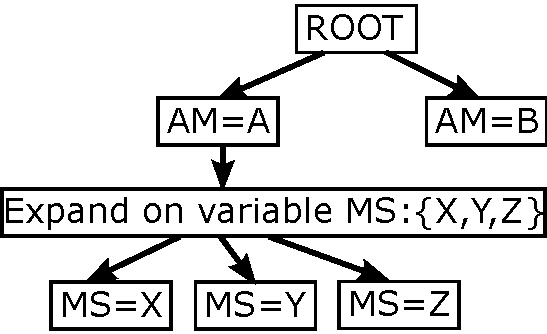
\includegraphics[width=\textwidth]{figures/expand_on_variable.pdf}
		\caption{}
		\label{fig:ExpandOnVariable}
	\end{subfigure}
	\hspace{1cm}
	\begin{subfigure}[b]{0.52\textwidth}
		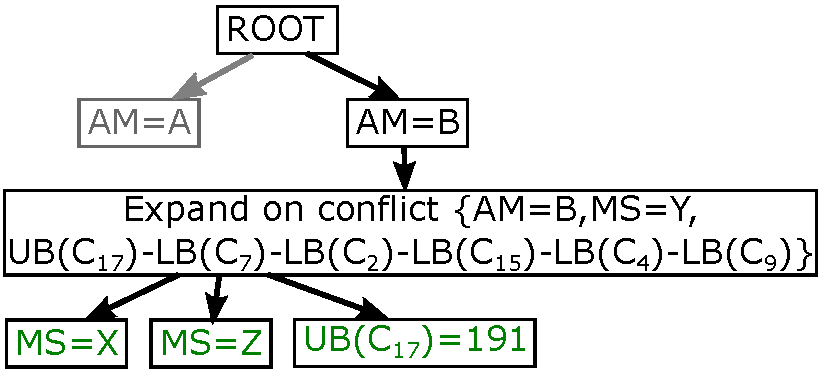
\includegraphics[width=\textwidth]{figures/expand_on_conflict.pdf}
		\caption{}
		\label{fig:ExpandOnConflict}
	\end{subfigure}
	\caption{Examples of expanding on variable and conflict}
\end{figure} 



If $\mathit{Cand}$ is complete, BCDR proceeds to check its consistency using function
\textsc{ConsistencyCheck} (Line 10). If no conflict is returned, $\mathit{Cand}$ will be
returned as the best relaxation for the input CCTP (Line 12). If a new conflict,
$\mathit{newConf}$, is detected by \textsc{ConsistencyCheck}, BCDR will record it in $C$
and put $\mathit{Cand}$ back to the queue for future expansions (Line 14,15), since it
now has one unresolved conflict.


\subsubsection{Conflict Learning From Consistency Checking}


Conflict learning is the key for resolving over-subscribed temporal plans. They
explain the cause of failure and provide guidance for computing necessary
relaxations. Previous approaches
\cite{bobby_csail_report_2005,Li05generalizedconflict}, including the discrete
relaxation version of BCDR
presented in Chapter 3, only extract the set of conflicting episodes and their
guard assignments as discrete conflicts.


\begin{mydef}
	A discrete conflict is a pair $\langle E,Guards\rangle$, where:
	\begin{itemize}
		\item $E$ is a set of conflicting constraints in the CCTP;
		\item $Guards$ is the set of guards assignments for all constraints in $E$;
	\end{itemize}
\end{mydef}


For example, the discrete conflict from the CCTP in Figure \ref{fig:example_cctp}
can be encoded as the following:\\

\begin{tabular}{m{2.5cm} m{11cm}}
	\textbf{E:} 	& \{$C_{17}$:$E$-$S\in[0,180]$; $C_7$:$B_A$-$S\in[30,50]$;
	$C_2$:$B_L$-$B_A\in[45,60]$;\\
	& $C_{15}$:$Y_A$-$B_L\in[21,25]$; $C_4$:$Y_L$-$Y_A\geq65$;
	$C_9$:$E$-$Y_L\in[30,32]$\}\\
	\textbf{Guards:} 	& \{$AM$=$B$; $MS$=$Y$\}\\
\end{tabular}\\

While computing continuous temporal relaxations, BCDR needs
conflicts of higher resolution, since it tries to resolve the conflict by
weakening the temporal bounds to the minimal extent. With the discrete
relaxation representation, we
can only learn about the constraints that are involved in the conflicts, but not
the amount of deviation required for their temporal bounds in order to resolve
the conflict. Therefore, we define a new representation of conflicts, called
\textbf{hybrid conflicts}, over the temporal bounds in episodes and their guard
assignments.


\begin{mydef}
	A hybrid conflict is a pair $\langle NCycles,Guards\rangle$, where:
	\begin{itemize}
		\item $NCycles$ is a set of linear expressions defined over temporal bounds of
		constraints, that forms a negative cycle in the equivalent distance graph of the
		CCTP;
		\item $Guards$ is the set of guards assignments for all constraints in $NCycles$;
	\end{itemize}
\end{mydef}


Each negative cycle in the $NCycles$ set is represented by a linear expression.
It represents a necessary constituent of the conflict, and is defined over the
lower and upper temporal bounds of episodes, with integer coefficients. BCDR
learns new conflicts iteratively from grounded CCTPs with different choices made.
Given a complete candidate that assigns all active discrete variables, Function
\textsc{ConsistencyCheck} evaluates the consistency of all activated temporal
constraints. The function implements the Bellman-Ford algorithm
\cite{bellman1956routing,ford1956network} for checking temporal consistency. If
the candidate plan is temporally inconsistent, the algorithm will return a
simple negative cycle as the cause of failure. We can extract the minimal
inconsistent set of constraints, also called $minimal conflict$
\cite{Liffiton_MUS_2005a}, using this simple negative cycle. For example, Figure
\ref{fig:negative_cycle_consistency} shows a simple negative cycle detected in
the TPN presented in Figure \ref{fig:example_cctp}: the mission time is too
tight for both tasks at site $B$ and $Y$.


\begin{figure}[h!]
	\centering	
	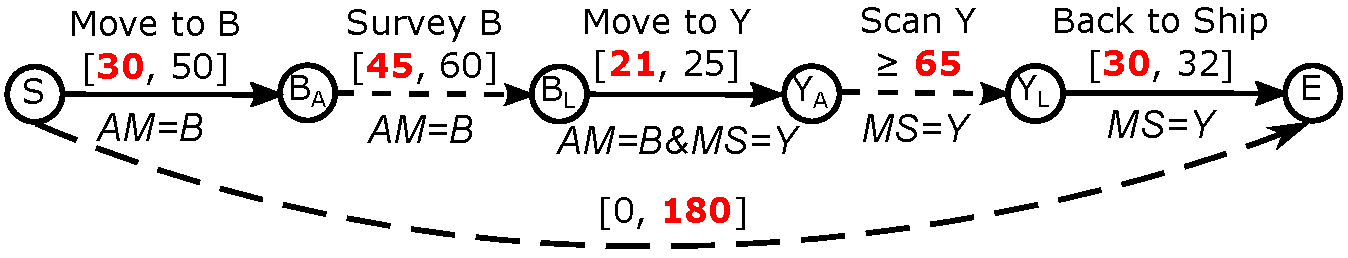
\includegraphics[width=0.9\textwidth]{figures/negative_cycle_consistency.pdf}	
	\caption{A negative cycle in Rich's mission CCTP (the guard assignments for each
		constraint are shown below them)}
	\label{fig:negative_cycle_consistency}
\end{figure}


Given the negative cycle, we can encode a hybrid conflict for it as: \\

\begin{tabular}{m{2.5cm} m{11cm}}
	\textbf{NCycles:} & \{\textsc{UB}($C_{17}$) - \textsc{LB}($C_{7}$) -
	\textsc{LB}($C_{2}$) - \textsc{LB}($C_{15}$) - \textsc{LB}($C_{4}$) -
	\textsc{LB}($C_{9}$);\}\\
	\textbf{Guards:} 	& \{$AM$=$B$; $MS$=$Y$\}\\
\end{tabular}\\

In summary, BCDR learns \textbf{hybrid conflicts} from temporally inconsistent
candidates, which are composed of the temporal bounds of constraints involved in negative
cycles and the guard assignments of these constraints. Each negative cycle is
encoded by a linear expression over the temporal bounds. Therefore, given the
original values of these temporal bounds, the value of this expression must
evaluate to negative.


\subsubsection{Generalized Conflict Resolutions}

Given a conflict detected in a CCTP, we can compute their resolutions and use
them to expand our search tree, such that future expansions of the candidates
will not enter the infeasible region represented by this conflict again. This is
the core principle behind conflict-directed search. Previous approaches generate
discrete relaxations by either flipping the assignments to the discrete
variables \cite{Williams_CDAstar_2002,Bailey_DAA_2005} or suspending temporal
constraints \cite{Moffitt_PCS_2005a}. BCDR generalizes the conflict resolution
to include both discrete and continuous relaxations: the discrete relaxations
deactivate constraints in conflicts by flipping their guard assignments, while
the continuous relaxations weakens the temporals bounds of them in order to
resolve the conflicts.


\begin{algorithm}[h!]
	\SetAlgoLined
	\SetKwFunction{Return}{return}
	\SetKwInput{Input}{Input}
	\SetKwInput{Output}{Output}
	\SetKwInput{Initialize}{Initialization}
	\SetKwInput{Algorithm}{Algorithm}
	\Indm
	\Input{A candidate to expand $\mathit{Cand}$ $\langle A,R,C_r,C_{cont}\rangle$ and an
		unresolved conflict $\mathit{currConf}$.}
	\Output{A set of expanded candidates $\mathit{newCands}$.}
	\Initialize{}
	\Indp
	{$\mathit{newCands}\leftarrow \{\}$}; collection of newly generated candidates\;
	{$\mathit{Confs}\leftarrow C_{cont}\cup \{\mathit{currConf}\}$; conflicts to be resolved
		continuously}\;
	{$A_{alter}\leftarrow \{\}$}; collection of alternative assignments for the ones in $\mathit{currConf}$\;
	\Indm
	\Algorithm{}
	\nonl\textsc{ExpandOnConflict}($\mathit{Cand}$,$\mathit{currConf}$)\\
	\Indp
	\For{$a\in \mathit{currConf}$}{
		$A_{alter}=A_{alter}\cup$\textsc{GetAlternatives}$(a)$\;
		\For{$a_l\in labels(a)$}{
			$A_{alter}=A_{alter}\cup$\textsc{GetAlternatives}$(a_l)$\;
		}
	}
	\For{$a_{extend}\in A_{alter}$}{
		\If{\textsc{notCompeting($A,a_{extend}$)}}{
			$\mathit{Cand_{new}}\leftarrow \langle A\cup\{a_{extend}\},R,C_r,C_{cont}\rangle$\;
			$\mathit{newCands}\leftarrow \mathit{newCands}\cup \{\mathit{Cand_{new}}\}$\;
		}
	}
	$E_{relax}\leftarrow$\textsc{ExtractConstraints}$(\mathit{Confs})$\;
	$f_{obj}\leftarrow\sum_{e\in E_{relax}}f_e(\Delta e)$\;
	$R_{new}\leftarrow$\textsc{Optimize}$(f_{obj},\langle
	E_{relax}\geq \textbf{0}\rangle )$\;
	\If{$R_{new}\neq null$}{
		$\mathit{Cand_{new}}\leftarrow\langle A,R_{new},C_r,C_{cont}\rangle $\;
		$\mathit{newCands}\leftarrow \mathit{newCands}\cup \{\mathit{Cand_{new}}\}$\;
	} 
	\Return $\mathit{newCands}$\;
	\caption{Function \textsc{ExpandOnConflict}}
	\label{alg:ExpandOnConflict}
\end{algorithm}



Given a candidate and a hybrid conflict, Function \textsc{ExpandOnConflict} generates
new candidates using the resolutions to the conflict (Algorithm
\ref{alg:ExpandOnConflict}). There are two stages in computing the resolutions:
First, we generate resolutions for the conflict by negating variable assignments
(Line 4-15). If a variable $p_i$ is conditioned on other assignments, in
addition to flipping the assignment to $p_i$, we can also negate its guards. This
deactivates the variable and resolves the conflict. Assuming that we have to make an additional decision on the imaging method, using either stereo camera or mono camera, for imaging methane seeps site Y. Then for a conflict that involves assignment $\mathit{IMAGE_Y=STEREO}$, given that we know variable $\mathit{IMAGE_Y}$ has label $MS=Y$, we can resolve the conflict by flipping the assignment to either $\mathit{IMAGE_Y}$ or $MS$: $\mathit{IMAGE_Y=MONO}$, $MS$=$X$ or $MS$=$Z$.


In the second stage, we compute the optimal continuous relaxation to the
relaxable temporal bounds (Line 16-22), which provides the lower bound on the
cost for resolving the conflict continuously. We formulate the relaxation as an optimization
problem with linear constraints (Line 16) and linear/quadratic objective
function (Line 17). The objective function is the minimization over the sum of
the relaxation costs of all relaxable constraints, as in (Equation \ref{eqn:rel_obj}).
The variables in this optimization problem are $LB_i'$ s and $UB_i'$ s, which
are the relaxed bounds for each relaxable temporal constraint. For relaxable
requirement constraints, their new temporal bounds must be no tighter than the
original bounds, as in (Equation \ref{eqn:rel_req}). The resolution constraints in
(Equation \ref{eqn:conf_res}) are added to ensure that all known conflicts are repaired
by the resolution. Given $m$ conflicts, the same number of resolution
constraints will be added, each representing the negation of one linear
expression in each conflict (Line 18).

\begin{problem}[Conflict resolution]
	\begin{align}
		&\phantom{=}	\min_{lb_i',ub_i'}\sum\limits_{i=1}^{|RE|}f_{e}(lb_i')+f_{e}(ub_i'); \label{eqn:rel_obj}\\
		s.t. &\phantom{=} lb_i'-lb_i \leq 0, \quad \phantom{=} ub_i'-ub_i \geq 0; \label{eqn:rel_req}\\
		&\phantom{=} Conflict_1 \geq 0; \phantom{=} Conflict_2 \geq 0;  ... \phantom{=} Conflict_m \geq 0 \label{eqn:conf_res}
	\end{align}
	\label{prob:conflict_resolution_consistency}
\end{problem}

For example, the conflict in (Figure \ref{fig:negative_cycle_consistency})
involves six temporal bounds. Among them, three are relaxable
($C_{17},C_2,C_4$)that can be relaxed. We can define the following optimization
problem for computing the optimal continuous relaxations to resolve this
conflict:


\begin{center}
	$min(f_e(ub_{C17}')+f_e(lb_{C2}')+f_e(lb_{C4}'))$;\\
	s.t. $ub_{C17}'-ub_{C17}\geq 0$; $lb_{C2}'-lb_{C2}\leq 0$; $lb_{C4}'-lb_{C4};\leq 0$\\
	$ub_{C17}'-lb_{C7}-lb_{C2}'-lb_{C15}-lb_{C4}'-lb_{C9}\geq 0$;\\	
\end{center}

The solution to the above optimization problem is a set of relaxed bounds of
$C_{17}$, $C_2$, and $C_4$ that resolves the conflict while minimizing the cost.
In this case, the best relaxation is: set $lb_{C4}'$ to 50 and $ub_{C17}'$ to
185. The cost is 27.5. In fact, this problem can also be viewed as a Simple
Temporal Problem with Preferences. \citeA{Khatib01temporalconstraint}
demonstrates that finding the optimal solution to a STPP with semi-convex
preferences is tractable. In real world applications, we may substitute
different optimization algorithms, depending on the preference functions, to
improve efficiency.


In this example, BCDR will generate three constituent relaxations for the hybrid
conflict: two new assignments derived from flipping guard assignments, and one
set of continuous relaxations for the temporal bounds. They are used to extend
the partial candidates so that future extensions of it will not run into the same
conflict again, as demonstrated in Figure \ref{fig:ExpandOnConflict}. When there are multiple unresolved conflicts for a candidate, BCDR is set to expand on the conflict with the least amount of variable assignments first (implemented in function \textsc{UnresolvedConflicts}): this will produce a smaller set of constituent relaxations, and allow a larger portion of the search space to be pruned.


\subsection{BCDR-U: Computing Relaxations that Restore Controllability}


As stated in the beginning of this section, for problems with uncertain
durations, such as CCTPUs, the consistency-based approach cannot find relaxation
that is robust to all possible outcomes of the uncertainty. Here, we
present the extension for conflict learning and resolution procedures that
accounts for uncontrollable duration, which allows BCDR to enumerate strongly
and dynamically controllable relaxations for CCTPUs. These changes are presented in Algorithm \ref{alg:bcdr_controllability}. First, \textsc{ControllabilityCheck} replaces the consistency check in BCDR
presented earlier. Depending on the type of solution required, it checks either
strong or dynamic controllability, and returns a conflict if the candidate
fails the test. The key is to learn conflicts from strong and dynamic
controllability checking algorithms, and the conflict could be a mixed set of
requirement constraints and uncertain duration. Second, Function
\textsc{ExpandOnConflict} is extended to handle conflicts with uncertain
durations, whose resolution may involve relaxing requirement constraints and
tightening uncertain constraints.


\begin{algorithm}[htb!]
	\SetAlgoLined
	\SetKwFunction{Return}{return}
	\SetKwInput{Input}{Input}
	\SetKwInput{Output}{Output}
	\SetKwInput{Initialize}{Initialization}
	\SetKwInput{Algorithm}{Algorithm}
	\SetKwIF{If}{ElseIf}{Else}{if}{then}{else if}{else}{endif}
	\Indm
	\Input{A CCTPU $T=\langle P,Q,V,V_r,E,E_u,RE,RE_u,L_p,L_e,f_p,f_e\rangle$.}
	\Output{Assignments and relaxations $\langle A,R_e,R_u,C_r,C_{cont}\rangle$ that maximizes $f_p-f_e$.}
	\Initialize{}
	\Indp{$\mathit{Cand}\leftarrow \langle A,R_e,R_u,C_r,C_{cont}\rangle $; the first
		candidate}\;
	{$Q\leftarrow\{\mathit{Cand}\}$; a priority queue that records candidates}\;
	{$C\leftarrow\{\}$; the set of all known conflicts}\;
	{$\mathit{currConf}\leftarrow \{\}, \mathit{newConf}\leftarrow \{\}$; the unresolved conflict that is being expanded on, and the newly discovered conflict. Each is a list of variable assignments and linear expressions}\;
	{$U\leftarrow V$; the list of unassigned controllable variables}\;
	\Indm
	\Algorithm{}
	\nonl\textsc{BCDR-U}($\mathit{T}$)\\
	\Indp
	\While{$Q\neq \emptyset$}{
		$\mathit{Cand}\leftarrow $Dequeue$(Q)$\;
		$\mathit{currConf}\leftarrow$\textsc{UnresolvedConflicts}$(\mathit{Cand},C)$\;
		\eIf{$\mathit{currConf}==null$}{
			\eIf{isComplete?$(\mathit{Cand},U)$}{
				$\mathit{newConf}\leftarrow$\textsc{ControllabilityCheck}$(\mathit{Cand})$;\\
				\eIf{$\mathit{newConf}==null$}{
					\Return $\mathit{Cand}$\;
				}{
				$C\leftarrow C\cup\{\mathit{newConf}\}$\;
				$Q\leftarrow Q\cup\{\mathit{Cand}\}$\;
			}			
		}{
		$Q\leftarrow Q\cup$\textsc{ExpandOnVariable}($\mathit{Cand},U$);\\
	}
}{
$Q\leftarrow$ $Q\cup$\textsc{ExpandOnConflict}($\mathit{Cand},\mathit{currConf}$);\\
}
}
\Return $null$\;
\caption{BCDR-U for solving CCTPUs}
\label{alg:bcdr_controllability}
\end{algorithm}


\subsubsection{Conflict Learning For Strong Controllability}


For CCTPs, a conflict is an inconsistent set of temporal bounds from controllable durations. It can
be detected by negative loop detection algorithms: a negative cycle in the
equivalent distance graph of a grounded CCTP can be mapped to a set of
conflicting constraints. This is because of the one-to-one mapping between the
distance edges and the lower/upper temporal bounds of constraints. However, this
method does not apply to controllability checking algorithms. Due to the
reduction procedures in both strong and dynamic controllability checking, the one-to-one mapping property is not preserved: during reductions,
new distance edges are created and added to the graph, and the weights of some
edges are modified. We cannot extract the sets of conflicting constraints from
the negative loops in reduced graphs directly.

The key to solve this issue is to understand what controllable and uncertain duration contributed to
each distance edge in the reduced graph. We name these constraints the
\textit{supporting constraints}. The supporting constraints for an edge include
the source constraint and the constraints that modify the weight of the edge
during reduction. We extend the polynomial time algorithm introduced by
\citeA{Vidal99handlingcontingency} with additional procedures for recording
supporting constraints during reductions (Algorithm \ref{alg:sc_conflict}). This
extension enables the algorithm to extract a conflict from a negative loop in
the reduced graph. The input to it is a grounded CCTPU without any unassigned
variables. There are three major steps in this algorithm: 

\begin{itemize}
	\item Map the grounded CCTPU to its equivalent distance graph (Line 1) and
	record the supporting constraints of each distance edge in the graph with its
	source, which is either an upper or lower bound of a temporal constraint.
	
	\item Reduce all non-contingent edges that start (Line 14) or end (Line 5) at an
	uncontrollable node using the triangular reduction rules (Figure \ref{fig:sc_reduction}). If constraint A is
	reduced to C through B, the supporting constraints of C will be updated to the
	union of the supporting constraints of A and B (Line 11, 20). 
	
	\item After the reductions, we run the Bellman-Ford algorithm on the reduced
	graph (Line 24). If a negative loop is detected, we collect the supporting
	constraints of all its edges into a set (Line 25) and return it as a conflict
	that makes the problem uncontrollable. Otherwise, the function returns null to
	indicate that the input CCTPU is strongly controllable.
\end{itemize}



\begin{algorithm}[ht!]	
	\SetAlgoLined
	\SetKwFunction{Return}{return}
	\SetKwInput{Input}{Input}
	\SetKwInput{Output}{Output}
	\SetKwInput{Initialize}{Initialization}
	\SetKwInput{Algorithm}{Algorithm}
	\SetKwIF{If}{ElseIf}{Else}{if}{then}{else if}{else}{endif}
	\Indm
	\Input{A grounded CCTPU $T=\langle V,E,E_u,L_e,L_p\rangle $.}
	\Output{A conflict $\langle A,E',Exp\rangle $ that makes $T$ uncontrollable}
	\Algorithm{}
	\nonl\textsc{ControllabilityCheck}($\mathit{T}$)\\
	\Indp
	$DG\leftarrow$\textsc{GetDistanceGraph}$(T)$;\\
	$ReductionQ\leftarrow$\textsc{NonContingentEdges}$(DG)$;\\
	\While{$ReductionQ\neq \emptyset$}{
		$\alpha\leftarrow $Dequeue$(ReductionQ)$\;
		\uIf{\textsc{End}$(\alpha)$ is uncontrollable}{
			$\beta\leftarrow$ \textsc{ContingentEdgeEndAt}$($\textsc{End}$(\alpha))$ //retrieve the contingent edge that ends at the end node of edge $\alpha$\;
			$\alpha'\leftarrow$ \textsc{Reduce}$(\alpha,\beta)$;\\
			$\gamma\leftarrow$\textsc{GetEdge}$($\textsc{Start}$(\alpha),$\textsc{Start}$(\beta))$;\\
			\If{\textsc{Weight}$(\alpha')<$\textsc{Weight}$(\gamma)$}{
				$\gamma\leftarrow \alpha'$;\\
				\textsc{Supports}$(\gamma)\leftarrow$ \textsc{Supports}$(\alpha,\beta)$;\\
				$ReductionQ\leftarrow ReductionQ\cup \gamma$;\\
			}
		}
		\uElseIf{\textsc{Start}$(\alpha)$ is uncontrollable}{
			$\beta\leftarrow$ \textsc{ContingentEdgeStartAt}$($\textsc{Start}$(\alpha))$ //retrieve the contingent edge that ends at the start node of edge $\alpha$\;
			$\alpha'\leftarrow$ \textsc{Reduce}$(\alpha,\beta)$;\\
			$\gamma\leftarrow$\textsc{GetEdge}$($\textsc{End}$(\beta),$\textsc{End}$(\alpha))$;\\
			\If{\textsc{Weight}$(\alpha')<$\textsc{Weight}$(\gamma)$}{
				$\gamma\leftarrow \alpha'$;\\
				\textsc{Supports}$(\gamma)\leftarrow$ \textsc{Supports}$(\alpha,\beta)$;\\
			}  		 	
		}{
		\textbf{endif}}
	
}
$NCycle\leftarrow$\textsc{Bellman-Ford}$(DG)$;\\
\Return \textsc{GetSupports}$(NCycle)$\;
\caption{Strong controllability checking algorithm}
\label{alg:sc_conflict}

\end{algorithm}

We demonstrate this process using a temporal network with four constraints
(Figure \ref{fig:sc_reduction_1}): A and B are uncertain durations; C and D are requirement constraints. First, we map the
network to its equivalent distance graph (Figure \ref{fig:sc_reduction_2}). Each
distance edge in the graph is labeled with its weight and supporting
constraints. The subscript after the constraint name, either U or L, specifies
if the distance edge is generated from the upper or lower bound of the
constraint.

\begin{figure}[ht!]
	\centering
	\begin{subfigure}[b]{0.235\textwidth}
		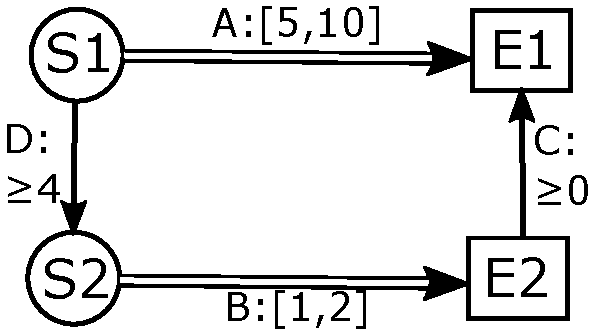
\includegraphics[width=\textwidth]{figures/sc_reduction_1.pdf}
		\caption{}
		\label{fig:sc_reduction_1}
	\end{subfigure}
	\begin{subfigure}[b]{0.235\textwidth}
		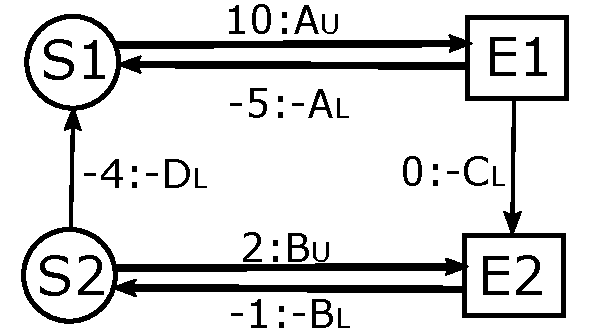
\includegraphics[width=\textwidth]{figures/sc_reduction_2.pdf}
		\caption{}
		\label{fig:sc_reduction_2}
	\end{subfigure}
	\begin{subfigure}[b]{0.22\textwidth}
		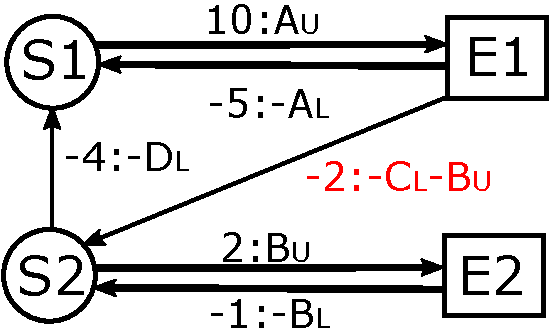
\includegraphics[width=\textwidth]{figures/sc_reduction_3.pdf}
		\caption{}
		\label{fig:sc_reduction_3}
	\end{subfigure}
	\begin{subfigure}[b]{0.26\textwidth}
		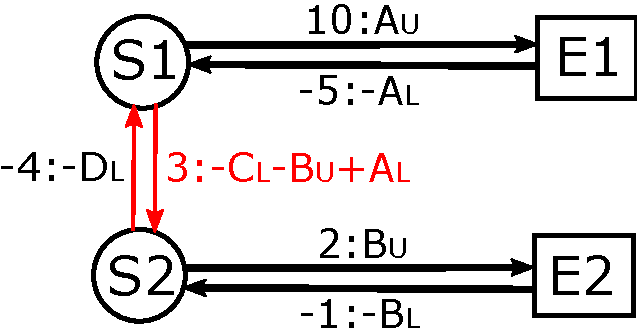
\includegraphics[width=\textwidth]{figures/sc_reduction_4.pdf}
		\caption{}
		\label{fig:sc_reduction_4}
	\end{subfigure}
	\caption{Supports recording during the triangular reduction for checking strong controllability}
	\label{fig:sc_reduction}
\end{figure}


There are two non-contingent edges in the graph, S2-S1 and E1-E2, and E1-E2
starts and ends at received nodes (denoted by squares in the graph). We first
reduce it using edge S2-E2, a contingent edge that shares the same end node with
E1-E2. The result is a new edge E1-S2 with weight -2 and supporting constraints
$C_L,B_U$, which are the union of the supporting constraints of E1-E2 and S2-E2
(Figure \ref{fig:sc_reduction_3}). Since E1-S2 starts at an received node, we
can further reduce it using E1-S1. The result is edge S1-S2 with weight 3 and
supporting constraints $C_L, B_U, A_L$ (Figure \ref{fig:sc_reduction_4}).


It can be seen from the reduced graph that there is a negative cycle of two
edges: S1-S2 and S2-S1. The negative cycle indicates that the original STNU is
not strongly controllable, and the supporting constraints of these two edges,
\{$A_L,B_U,C_L,D_L$\}, are in conflict and cause the failure. The linear
expression in the $NCycles$ component of this conflict is
$-LB(D)-LB(C)-UB(B)+LB(A)$, whose value is -1 without any relaxations to the
temporal bounds.


Using this algorithm for checking strong controllability and extracting
conflicts does not add much overhead: it takes the same order of magnitude in
time compared to consistency checking algorithms. Given a problem with $V$
events and $E$ temporal constraints, there will be at most $2E$ reductions and support
constraint recordings. The time complexity of strong controllability is thus the
same order of magnitude as consistency checking: both are dominated by the
$O$($VE$) negative cycle detection.


\subsubsection{Conflict Learning For Dynamic Controllability}

Our approach for learning conflicts from dynamic controllability checking
algorithm is similar to that for strong controllability. We extend the
\textsc{fastDCcheck} algorithm, introduced by \citeA{Morris_astructural}, with additional
steps in its reduction procedures to record the supporting constraints of reduced
edges. Its pseudo code is presented in Algorithm \ref{alg:dc_conflict}.

\begin{algorithm}[ht!]
	\SetAlgoLined
	\SetKwFunction{Return}{return}
	\SetKwInput{Input}{Input}
	\SetKwInput{Output}{Output}
	\SetKwInput{Initialize}{Initialization}
	\SetKwInput{Algorithm}{Algorithm}
	\SetKwIF{If}{ElseIf}{Else}{if}{then}{else if}{else}{endif}
	\Indm
	\Input{A grounded CCTPU $T=\langle V,E,E_u,L_v,L_p\rangle $.}
	\Output{A conflict $\langle A,E',Exp\rangle $ that makes $T$ uncontrollable}
	\Algorithm{}
	\nonl\textsc{ControllabilityCheck}($\mathit{T}$)\\
	\Indp
	$DG\leftarrow$\textsc{GetNormalDistanceGraph}$(T)$;\\
	\For{1 to K}{ 
		$NCycle\leftarrow$\textsc{AllMaxConsistent}$(DG)$;\\
		\eIf{$NCycle==null$}{
			\For{$E$ in \textsc{LowerCaseEdges}$(DG)$}{
				$moatPaths\leftarrow$\textsc{Propagate}$(E)$;\\
				\For{$Path$ in $moatPaths$}{
					$E'\leftarrow$\textsc{Reduce}$(E$,$Path)$;\\
					\textsc{Supports}$(E')\leftarrow$ \textsc{Supports}$(E,Path)$;\\
					\textsc{AddToGraph}$(E',DG)$
				}
			}
		}{
		\Return \textsc{GetSupports}$(NCycle)$\;
	}
}	
$NCycle\leftarrow$\textsc{AllMaxConsistent}$(DG)$;\\
\Return \textsc{GetSupports}$(NCycle)$\;
\caption{Modified \textsc{fastDCcheck} algorithm for learning conflicts from uncontrollable networks}
\label{alg:dc_conflict}
\end{algorithm}


As proved by \citeA{Morris_astructural}, an STNU is dynamically controllable if
and only if it does not have a semi-reducible negative cycle. The
\textsc{fastDCcheck} algorithm is designed based on this theorem. It converts
the STNU to an equivalent distance graph of normal form (Line 1) and identifies
all negative paths that start with a lower-case edge, called \textit{moat
	paths}, through propagations (Line 6). The input STNU is determined to be
dynamically controllable if none of these negative paths leads to a
semi-reducible negative cycle (Line 3, 17). The check requires at most $K$
iterations (Line 2), where $K$ is the number of lower case edges in the
equivalent distance graph of the STNU.


During the reduction of moat paths, we record the supporting constraints for
each reduced edge (Line 9). If the \textsc{AllMaxConsistent} function, which
implements the Bellman-Form algorithm on all non-lower case edges, captures a
negative cycle in the reduced graph, it will return a conflict that collects the
supporting constraints of all edges in the cycle. There are five types of
reductions in this procedure \cite{Morris05temporaldynamic,Morris_astructural},
and the support recording process is demonstrated for each of them in Figure \ref{fig:DCReduction}.


\begin{figure}[ht!]
	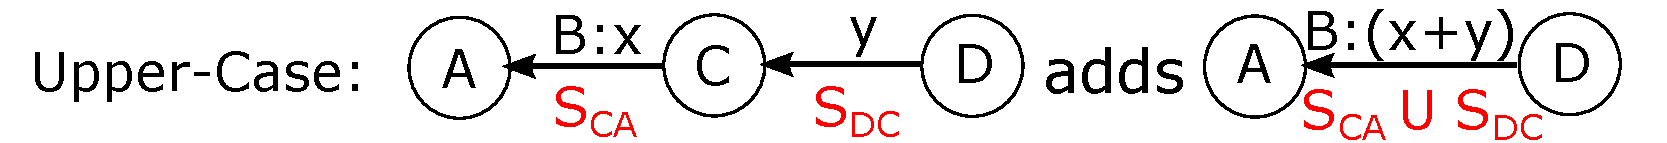
\includegraphics[width=0.8\textwidth]{figures/DC_reductions/UpperCase.pdf}  
	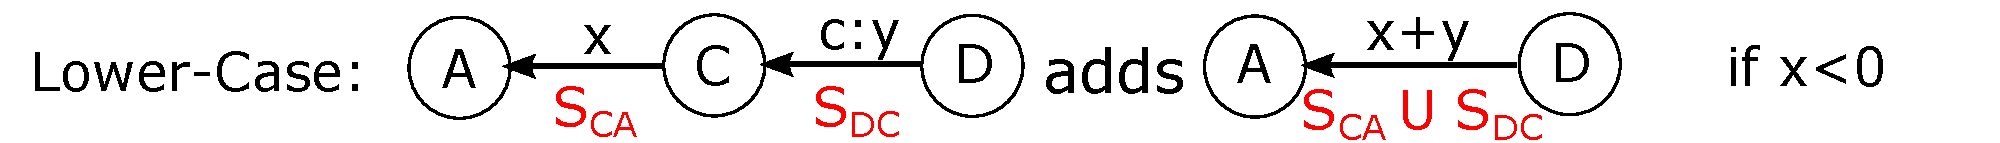
\includegraphics[width=0.96\textwidth]{figures/DC_reductions/LowerCase.pdf}  
	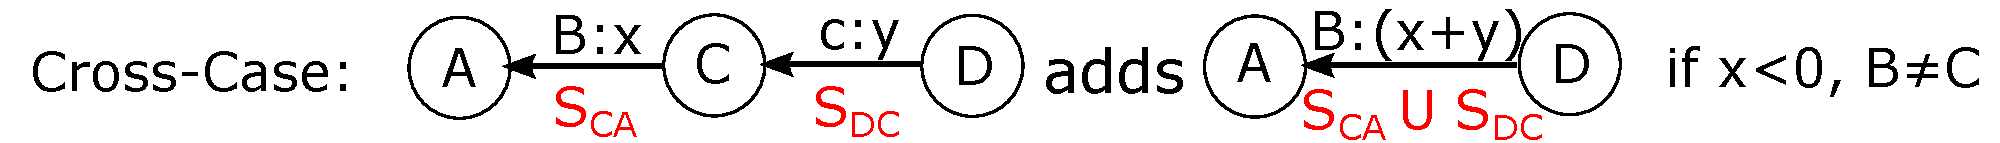
\includegraphics[width=0.96\textwidth]{figures/DC_reductions/CrossCase.pdf}
	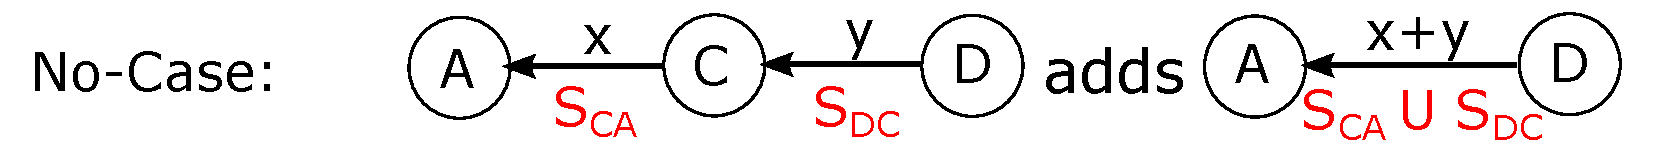
\includegraphics[width=0.8\textwidth]{figures/DC_reductions/NoCase.pdf}
	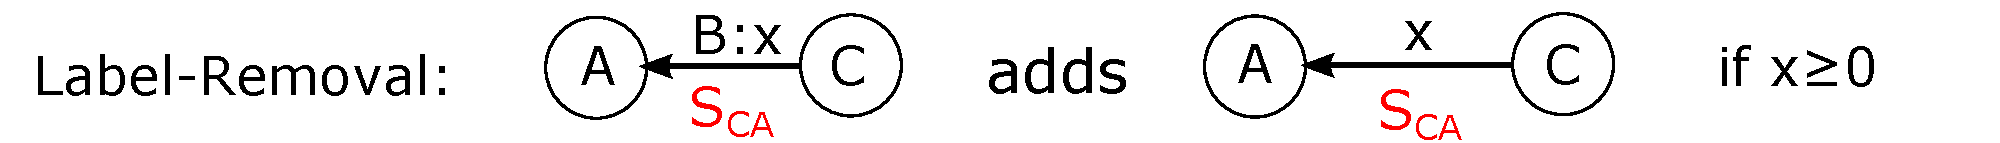
\includegraphics[width=0.96\textwidth]{figures/DC_reductions/LabelRemoval.pdf}
	\caption{Record supporting constraints during the \textsc{fastDCcheck} reductions}
	\label{fig:DCReduction}
\end{figure}


Next, we demonstrate the conflict learning process using a simple dynamic
controllability checking example (Figure \ref{fig:dc_reduction1}). There are three events,
E1, E2 and E3, in this example STNU. These events are connected by two
constraints A and B: A is an uncertain duration with a bound of [10,15], while B
is a requirement constraints with a bound of [1,1]. The first step of
controllability checking is to map the STNU to a normalized form
\cite{Morris05temporaldynamic}, which decouples the lower bounds from each
uncertain duration (Figure \ref{fig:dc_reduction2}). We can then generate the
equivalent distance graph using the normalized STNU. Note that each distance
edge in the graph, including conditional edges, is labeled with a linear
expression over constraints. The expression encodes the source of an
distance edge's weight value, such as the example in Figure
\ref{fig:dc_reduction3}.


\begin{figure}[htb]
	\centering
	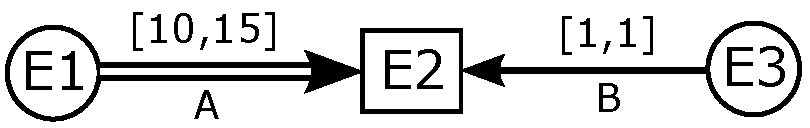
\includegraphics[width=0.45\textwidth]{figures/DC_reductions/dc_reduction1.pdf}
	\caption{The original STNU}
	\label{fig:dc_reduction1}
\end{figure}

\begin{figure}[htb]
	\centering
	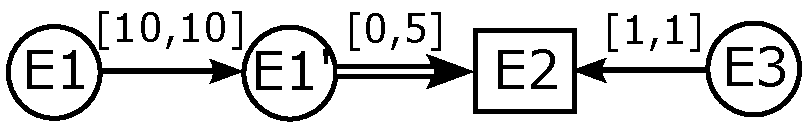
\includegraphics[width=0.45\textwidth]{figures/DC_reductions/dc_reduction2.pdf}
	\caption{The normalized STNU}
	\label{fig:dc_reduction2}
\end{figure}

\begin{figure}[htb]
	\centering
	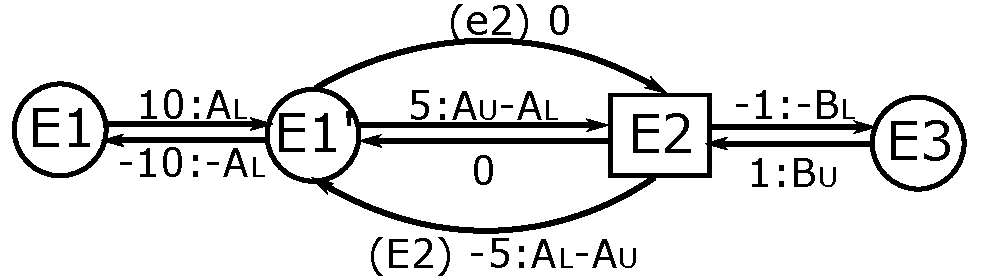
\includegraphics[width=0.6\textwidth]{figures/DC_reductions/dc_reduction3.pdf}
	\caption{The equivalent distance graph of the STNU}
	\label{fig:dc_reduction3}
\end{figure}

The next step is to identify and reduce all moat paths in the distance graph using the
iterative method introduced by \citeA{Morris_astructural}. In this example, there
is only one valid moat path: $E1'\rightarrow E2\rightarrow E3$. This path has a
negative weight, starts with a lower-case edge, and can be reduced to a single
edge using a lower-case reduction. The reduced edge (represented by a dotted
arrow in Figure \ref{fig:dc_reduction4}) of the moat path has a weight of -1, and
is supported by a linear expression, $-B_L$, that combines the expressions of all edges
in the moat path.


\begin{figure}[htb]
	\centering
	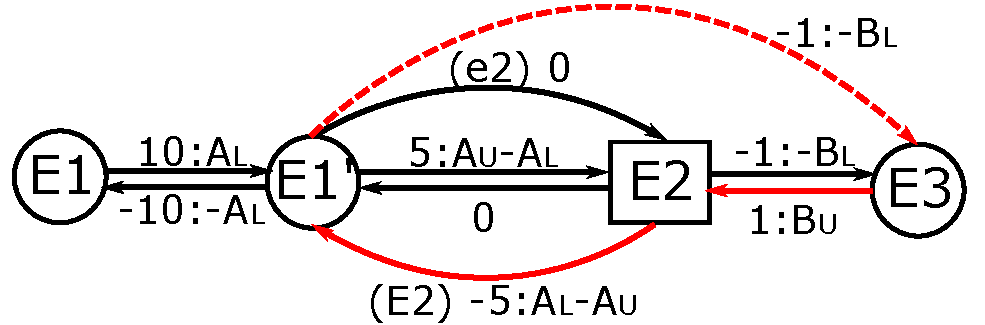
\includegraphics[width=0.6\textwidth]{figures/DC_reductions/dc_reduction4.pdf}
	\caption{The distance graph with a reduced edge}
	\label{fig:dc_reduction4}
\end{figure}


After all applicable reductions, the final step is to run
\textsc{AllMaxConsistent} check on the resulting graph, which checks the
consistency of the graph without the lower-case edges. It will
reveal any negative cycle in the reduced graph, whose existence indicates that
the STNU is not dynamically controllable. In this example, one negative cycle
can be detected that contains edge $E3\rightarrow E2$, $E2\rightarrow E1'$, and
the reduced edge $E1'\rightarrow E3$. From this cycle, we can identify the
linear expression that caused this conflict from all distance edges in the
cycle: $UB(B)+LB(A)-UB(A)-LB(B) \le 0$. In addition, there is another subtle but
necessary element of this conflict: the reduction that adds edge $E1'\rightarrow
E3$. The negative cycle would not exist without this reduced edge. Therefore,
the expression that supports the reduction, $-LB(B) \le 0$, which guarantees a
negative weight for the moat path, is included in the conflict. The conflict we
can extract from the STNU is a conjunction of two linear expressions,
\{$B_U+A_L-A_U-B_L$;$-B_L$\},. Making any one of them non-negative will
resolve this conflict.


In summary, learning conflicts from dynamic controllability checking with
\textsc{fastDCcheck} requires recording the supporting expression for each
distance edge and reduction. Once a negative cycle is detected, we can extract a
conflict by collecting (1) the expressions for each edge in the cycle; and (2)
the expressions required by the reductions that added edges to the cycle. The
conflict is a conjunction of these linear expressions, which are all negative
and defined over the temporal bounds of constraints. 


Currently, extracting conflicts from dynamic controllability checking is
significantly harder than that for strong controllability, even though the extra
time and space required by recording supports during reductions does not
increase the overall complexity of the algorithm. The \textsc{fastDCcheck}
algorithm is currently the second fastest DC checking algorithm with a
complexity of $O(N^4)$, which is an order of magnitude higher than checking
strong controllability. To improve run-time efficiency, the algorithm can be
terminated and return true after a no-reduction iteration. This is similar to
the implementation presented by \citeA{Morris05temporaldynamic}, and will not affect the
correctness of the results. The integration of BCDR with a cubic DC checking
algorithm introduced by \citeA{morris2014dynamic}, is expected to further improve
performance and is part of our future work to explore.


\subsubsection{Resolving Conflicts with Uncontrollable Durations}

As described in the beginning of this subsection, both BCDR-U(SC) and BCDR-U(DC) algorithms use the resolutions to
unresolved conflicts to expand the search tree. For CCTPUs, there are three
options for resolving its conflicts, which may include both controllable
constraints and uncertain duration:

\begin{itemize}
	\item Flipping the guard assignments to deactivate constraints.
	
	\item Relax the temporal bounds of requirement constraints.
	
	\item Tighten the temporal bounds of uncertain durations.
\end{itemize}


The conflict resolution process for CCTPUs, similar to the one for CCTPs, is 
separated into two stages. The first stage is identical to that for CCTPs: we
look for alternative assignments that can deactivate one or more constraints in
the conflict, and use them to generate new candidates.

The second stage implements option 2 and 3. We compute the continuous
relaxations to the temporal bounds in the conflicts. The linear expressions
in each conflict's negative cycles provide guidance for \textsc{ExpandOnConflict} to resolve
over-constrained problems. A conflict is eliminated if any of its linear
expressions is made non-negative. For example, we can resolve the conflict in
Figure \ref{fig:dc_reduction4} using the following two approaches:


\begin{itemize}
	\item Set $B_U+A_L-A_U-B_L \geq 0$, e.g. increasing $A_L$ to 15.
	\item Set $-B_L \geq 0$, e.g. lowering  $B_L$ to 0.
\end{itemize}


Intuitively, to resolve a conflict we can directly require the weight of a
previously negative cycle to be non-negative, or we can make sure the reduction
which adds an edge never occurs. This choice in conflict resolution is unique to
dynamic controllability conflicts: a hybrid conflict from consistency or strong
controllability checking only introduces one linear expression. This choice
provides more flexibility in conflict resolution, although it also increases the
complexity of the problem: to compute the optimal resolutions, BCDR-U(DC) may
need to evaluate all possible repairs for all conflicts. The search branches
each time BCDR-U(DC) expands on a conflict. If a quick response is desired by
the user, BCDR-U(DC) should be implemented with an anytime search strategy.


Once an expression is selected for each conflict, we can again formulate a
constraint optimization problem and compute the resolutions using an
optimization solver in polynomial time, assuming that the objective function
remains semi-convex. There are two categories of variables in the optimization
problem: relaxed lower and upper bounds for requirement constraints ($lb_i'$ and
$ub_i'$) and tightened lower and upper bounds for uncertain durations
($lb_{uj}'$ and $ub_{uj}'$). These are given in Problem \ref{prob:conflict_resolution_controllability}.

\begin{problem}[Conflict resolution with set-bounded uncertain durations]
	\begin{align}
		&\phantom{=}	\min_{lb_i',ub_i',lb_{uj}',ub_{uj}'}\sum\limits_{i=1}^{|RE\backslash RE_u|}f_{e}(lb_i')+f_{e}(ub_i')+\sum\limits_{j=1}^{|RE_u|}f_{e}(lb_{uj}')+f_{e}(ub_{uj}');\\
		s.t. &\phantom{=} lb_i'-lb_i \leq 0, \quad \phantom{=} ub_i'-ub_i \geq 0; \\
			&\phantom{=} lb_{uj}'-lb_{uj} \geq 0, \quad \phantom{=} ub_{uj}'-ub_{uj} \leq 0, \quad \phantom{=} ub_{uj}'-lb_{uj}' \geq 0; \label{eqn:unc_bds}\\
			&\phantom{=} Conflict_1 \geq 0; \phantom{=} Conflict_2 \geq 0;  ... \phantom{=} Conflict_m \geq 0;
	\end{align}
	\label{prob:conflict_resolution_controllability}
\end{problem}
	

The constraints in the optimization problem enforce the necessary properties.
For CCTPUs, we have an additional set of constraints: for lower and upper bound
variables of uncertain durations, their value must be within the range defined
by the original bounds, and the new lower bound is smaller than the new upper
bound, encoded by (\ref{eqn:unc_bds}). For example, given the conflict in Figure
\ref{fig:dc_reduction1}, the relaxed bounds for uncertain duration $A$, $lb_{uA}'$
and $ub_{uA}'$, must follow $10 \leq lb_{uA}' \leq ub_{uA}' \leq 15$.


\subsection{BCDR-C: Computing Chance-constrained Relaxations}

Finally, we present the extension to the BCDR algorithm, called BCDR-C, that
allows it to resolve over-constrained cc-pCCTPs. The extension leverages ideas
presented by \citeA{Fang_AAAI_2014} for grounding probabilistic Simple Temporal Problems
(pSTPs) into deterministic STNUs, and uses the conflict-directed framework for
efficient conflict detection and resolution. Given a cc-pCCTP, BCDR-C enumerates
feasible solutions in best-first order: a solution is a complete set of assignments and a collection of relaxations
for temporal bounds and chance constraint. Each resolution supports a
grounded STNU whose probability of failure is bounded by the relaxed chance
constraint. This requires the conflict-directed approach to support both
relaxation and risk allocation: given the grounded STNU of a cc-pCCTP that
represents a specific set of choices and risk allocation, BCDR-C will identify
the conflicts between constraints and use their resolutions to guide the search
towards feasible risk allocation and constraint relaxation. The two key
modifications from BCDR-U to BCDR-C are the following:


\begin{itemize}


	\item First, an additional step of risk-allocation is required for grounding
	the probabilistic input problem to a STNU. This allows us to check the
	feasibility and extract conflicts between constraints using the algorithms developed for STNUs.

	\item Second, in addition to flipping assignments and relaxing temporal bounds, the conflict resolution step can also adjust risk allocation over uncertain durations in order to resolve all known conflicts while maintaining
	the risk taken. Note that this step may
	require a non-linear optimization solver if the probabilistic distribution of
	any uncertain duration is non-linear.

\end{itemize}



\begin{algorithm}[h!]
	\SetAlgoLined
	\SetKwFunction{Return}{return}
	\SetKwInput{Input}{Input}
	\SetKwInput{Output}{Output}
	\SetKwInput{Initialize}{Initialization}
	\SetKwInput{Algorithm}{Algorithm}
	\SetKwIF{If}{ElseIf}{Else}{if}{then}{else if}{else}{endif}
	\Indm
	\Input{A cc-pCCTP $T = \langle P, Q, V, V_r, E, E_d, RE, L_e, L_p, f_p, f_e, \Delta_t,r\Delta_t,f_\Delta\rangle$.}
	\Output{A solution $\langle A,R_e,\Delta'_t,N_{alloc},C_r,C_{cont}\rangle$ that maximize
		$f_{p}-f_{e}-f_\Delta$.}
	\Initialize{}
	\Indp{$\mathit{Cand}\leftarrow \langle A=\emptyset,R_{e}=\emptyset,\Delta_t,N_{default},C_r=\emptyset,C_{cont}=\emptyset\rangle $; the
		first candidate with the default risk allocation, and empty sets for assignments, relaxations and continuously resolved conflicts}\;
	{$Q\leftarrow\{\mathit{Cand}\}$; a priority queue of candidates}\;
	{$C\leftarrow\{\}$; the set of all known conflicts}\;
	{$\mathit{currConf}\leftarrow \{\}, \mathit{newConf}\leftarrow \{\}$; the unresolved conflict that is being expanded on, and the newly discovered conflict. Each is a list of variable assignments and linear expressions}\;
	{$U\leftarrow V$; the list of unassigned controllable variables}\;
	\Indm
	\Algorithm{}
	\nonl\textsc{BCDR-C}($\mathit{T}$)\\
	\Indp
	\While{$Q\neq \emptyset$}{
		$\mathit{Cand}\leftarrow $Dequeue$(Q)$\;
		$\mathit{currConf}\leftarrow$\textsc{UnresolvedConflict}$(\mathit{Cand},C)$\;
		\eIf{$\mathit{currConf}==null$}{
			\eIf{isComplete?$(\mathit{Cand},U)$}{
				$\mathit{newConf}\leftarrow$\textsc{ControllabilityCheck}$(\mathit{Cand})$;\\
				\eIf{$\mathit{newConf}==null$}{
					\Return $\mathit{Cand}$\;
				}{
					$C\leftarrow C\cup\{\mathit{newConf}\}$\;
					$Q\leftarrow Q\cup\{\mathit{Cand}\}$\;
				}
			}{
				$Q\leftarrow Q\cup$\textsc{ExpandOnVariable}($\mathit{Cand},U$);\\
			}			
		}{
			$Q\leftarrow$ $Q\cup$\textsc{\textsc{ExpandOnConflictAndAllocateRisk}}($\mathit{Cand},\mathit{currConf}$);\\
		}
	}
	\Return $null$\;
\caption{BCDR-C algorithm for resolving cc-pCCTPs}
\label{alg:bcdr_chance_constraints}
\end{algorithm}


We first present an overview of the algorithm that highlights the modifications,
then discuss the risk-allocation and chance constraint relaxation procedures in
detail. The pseudo code of the chance-constrained version of BCDR-C is presented
in Algorithm \ref{alg:bcdr_chance_constraints}. Similar to the previous two
versions, we implement BCDR-C with a priority queue for enumerating resolutions
in best-first order. The algorithm starts with an empty candidate (Line 1) that
has no assignments or relaxations over temporal constraints ($A$ and $R_{e}$)
and chance constraint ($\Delta_t$), and empty sets of resolved conflicts
($C_r$) and continuously resolved conflicts ($C_{cont}$). The candidate is associated with a default risk allocation over all
probabilistic uncertain durations, which is represented by a CCTPU
($N_{default}$). The initial allocation is computed from a non-linear solver and
is conservative enough to satisfy the chance constraint. For example, we can
compute the initial allocation by solving \ref{prob:conflict_resolution_cc}
without any linear constraints from conflicts.  The initial candidate is the
only element in the queue before search starts (Line 2).


Within the main loop, BCDR-C first dequeues the best candidate (Line 6) and
checks if it resolves all known conflicts (Line 7). If not, a conflict
$\mathit{currConf}$ will be returned by function \textsc{UnresolvedConflict}. The
unresolved conflict is then used for expanding $\mathit{Cand}$ (Line 21). All child
candidates returned by function \textsc{ExpandOnConflictAndAllocateRisk} resolve
$\mathit{currConf}$ while satisfying the chance constraints. The function also computes
the risk allocation over probabilistic temporal durations for each candidate,
which is added back to the queue for future evaluation and expansion.


If $\mathit{Cand}$ resolves all known conflicts, BCDR-C will proceed to check the
controllability of its grounded CCTPU (function \textsc{ControllabilityCheck},
Line 8). BCDR-C(SC) implements this function with a strong controllability checking algorithm, while BCDR-C(DC)'s function implements dynamic controllability checking. If the grounded network passes the check, $\mathit{Cand}$ will be returned as the best resolution to the
cc-pCCTP (Line 12). Otherwise, a new conflict will be returned by this function
and recorded for expanding candidates (Line 14). $\mathit{Cand}$ will also be added back
to $Q$ since it now has an unresolved conflict (Line 15).

Similar to BCDR and BCDR-U, every solution returned by BCDR-C is valid in that
they have a feasible risk-allocation and pass the strong or dynamic
controllability check, hence it is easy to prove the algorithm's soundness. On
the other hand, unlike BCDR and BCDR-U, BCDR-C is not a complete algorithm in
that it may fail to return a solution for some cc-pCCTPs that do have feasible
relaxations. This is a result of its conservative risk allocation procedure. We
take a union bound approach when calculating the total risk taken across the
temporal bounds allocated for all probabilistic durations. It guarantees that
the solution returned will operate within the specified risk-bound. However, the
conservation causes BCDR-C to overestimate the risk taken. As a result, it may
not be able to find a feasible risk allocation for problems with tight
risk-bounds, even if one may exist. We will discuss more details on this issue
in the following section.



\subsubsection{Risk Allocation and Constraint Relaxation}

Conflicts provide guidance for BCDR-C to resolve over-constrained problems. Given
a set of conflicts, we formulate a constrained optimization problem and compute
the resolutions using a non-linear optimization solver. To resolve a conflict we
can require the weight of any of its linear expressions to be
non-negative. There are three categories of variables in the optimization problem: relaxations
for temporal constraints ($lb'_{i}$ and $ub'_{i}$), relaxations for chance
constraint ($\Delta'_t$), and the allocation of lower and upper bounds for
probabilistic durations ($lb'_{pj}$ and $ub'_{pj}$). Each category of variables
represents a type of conflict resolution: re-allocating risk over probabilistic
durations, relaxing the chance constraint, and relaxing temporal constraints. These
are given in Problem \ref{prob:conflict_resolution_cc}.

\begin{problem}[Conflict resolution with chance constraints and probabilistic durations]
	\begin{align}
	&\phantom{=}	\min_{\Delta'_t,{lb_i',ub_i'}}f_\Delta(\Delta'_t-\Delta_t)+\sum\limits_{i=1}^{|RE|}f_{e}(lb_i') + f_{e}(ub_i');
	\label{eqn:obj}\\
	s.t. 	&\phantom{=}	lb'_{pj} - ub'_{pj} < 0   \label{eqn:prob_bds}\\
	&\phantom{=} lb_i'-lb_i \leq 0, \quad ub_i'-ub_i \geq 0; \label{eqn:relax_req}\\
	&\phantom{=} Conflict_1 \geq 0; \phantom{=} Conflict_2 \geq 0;  ... \phantom{=} Conflict_m \geq 0; \label{eqn:conf_res_cc}\\
	&\phantom{=}	\sum_{r_j\in R_d}\textsc{Risk}(lb'_{pj},ub'_{pj}) \leq \Delta'_t, \quad \Delta'_t \in \left[\Delta_t,1\right) \label{eqn:cc}
	\end{align}
	\label{prob:conflict_resolution_cc}
\end{problem}

The constraints in the optimization problem enforce the necessary properties.
For lower and upper bound variables of probabilistic durations, their value can
be assigned as long as the lower bound is smaller than the upper bound,
encoded by (\ref{eqn:prob_bds}). For relaxable requirement constraints, their new
temporal bounds must be no tighter than the original bounds, as in
(\ref{eqn:relax_req}). For requirement constraints that are not relaxable, their
temporal bounds remain unchanged (omitted from the encoding).


The resolution constraints in (\ref{eqn:conf_res_cc}) are added to ensure that
all known conflicts are repaired by the resolution, similar to those in Problems
\ref{prob:conflict_resolution_consistency} and \ref{prob:conflict_resolution_controllability}.. Given $m$ conflicts, the same number
of resolution constraints will be added, each representing one linear expression
in each conflict. Finally, we add a risk allocation constraint to ensure that
the risk taken meets the chance constraint. This constraint is defined over the
lower and upper bound variables of all probabilistic durations. Given
distributions of each probabilistic duration and the uncertainty bounds chosen,
the \textsc{Risk} function computes the probability mass of the regions outside
the uncertainty bounds. BCDR-C uses the union bound to upper-bound the total
risk taken across all uncertain durations, as this does not rely on assumptions
of independence. If the chance constraint is relaxable, we further require that
the relaxed chance constraint is lower bounded by the original chance
constraint, and upper bounded by 1. This gives us the flexibility to make
trade-offs between risk and performance, if no solution can be found that
resolves all conflicts while meeting the current chance constraint. These are
described by (\ref{eqn:cc}).


The objective function, given in (\ref{eqn:obj}), is defined over $f_\Delta$ and
$f_{e}$ for minimizing the cost of temporal and chance constraint relaxations.
In the optimization problem, all domain and conflict resolution constraints are
linear, while the chance constraint may be non-linear depending on the
probabilistic distributions. BCDR-C uses the SNOPT optimization package
\cite{Wachter06onthe} to solve Problem \ref{prob:conflict_resolution_cc} and
compute optimal constraint relaxations and risk allocations. If a solution is
returned by SNOPT, function \textsc{ExpandOnConflict} will construct a new
candidate with its relaxations for temporal and chance constraints. This
candidate will then be added as a new branch to BCDR-C's search tree, similar to
the process in Algorithms \ref{alg:bcdr} and \ref{alg:bcdr_controllability}. 

%For
%problems with a mixed set of set-bounded and probabilistic durations, this
%relaxation procedure will still work: we just need to include Equation
%\ref{eqn:unc_bds} for variables from set-bounded uncertain durations in our
%optimization problem. Note that these variables will not be included while
%evaluating the risk taken, hence they are not part of the risk allocation
%constraint (Equation \ref{eqn:cc}).


Finally, we would like to mention one limitation of BCDR-C on resolving
cc-pCCTPs. In many real-world scenarios, people may want to impose different chance
constraints over different subsets of uncertain durations. The current
implementation of BCDR-C, especially the chance-constrained relaxation
procedure, only supports a single chance constraint. It is unable to impose
different risk bounds on different sets of constraints while computing new
relaxations and risk allocations. Constraints covered by different risk bounds
may appear in the same conflict, and it is not clear how to distribute the risk
to multiple chance constraints during conflict resolution. The solutions to
these issues are part of our future work to explore.


\subsection{Incorporating User Inputs as Hybrid Conflicts}  


As demonstrated in Section 2, the user can add additional inputs given an
unsatisfying solution, or requirements he/she forgot to encode in the original
problem. BCDR can incorporate them into its search process as a hybrid conflict,
such that all future candidate solutions will respect them. In total, given a
solution, three types of inputs can be accepted by BCDR:

\begin{itemize}
	
	
	\item Rejection of an assignment, such as ``I do not want to visit the methane seeps
	site X".
	
	
	\item Rejection of a continuous temporal relaxation, such as ``The mission duration must be
	within 4 hours".
	
	
	\item Rejection of a chance constraint relaxation, such as ``I cannot take more
	than a 5\% risk of violating any constraints".
	
\end{itemize}


BCDR utilizes the conflict-directed approach to efficiently adapt to these
inputs. Instead of modifying the input problem and restarting the search process from
the beginning, it will record the input as a new conflict and add it to the
known conflicts list. The above three types of inputs will be recorded as the
following conflicts:


\begin{itemize}
	
	\item Rejection of an assignment $X=a$: a new conflict $X=a$ will be created
	and added to BCDR's conflict collection, such that it will not appear again in
	any future solutions.
	
	
	\item Rejection of a temporal relaxation $lb'_i=a$ or $ub'_i=b$: a new
	hybrid conflict with linear expression $lb'_i-a \geq 0$ or $b-ub'_i \geq 0$ will be added to
	BCDR's conflict collection, such that all future relaxations for $lb'_i$ or
	$ub'_i$ will be bounded by $a$ and $b$, respectively.
	
	
	\item Rejection of a chance constraint relaxation, $\Delta'_t = a$: update the
	domain of variable to $\Delta'_t \in [0,a]$. There is no need to generate new
	conflict since the chance constraint applied to all candidate solutions, and we
	allow one and only one chance constraint in each problem.
	
\end{itemize}


\begin{algorithm}[h!]
	
	\SetAlgoLined
	\SetKwFunction{Return}{return}
	\SetKwInput{Input}{Input}
	\SetKwInput{Output}{Output}
	\SetKwInput{Initialize}{Initialization}
	\SetKwInput{Algorithm}{Algorithm}
	\SetKwIF{If}{ElseIf}{Else}{if}{then}{else if}{else}{endif}
	\Indm
	\Input{$T$: A CCTP, CCTPU or cc-pCCTP.}
	\Output{$Sol$: A valid relaxation, or $null$ is none exists for the input problem.}
	\Initialize{}
	\Indp{$C\leftarrow\{\}$; the set of all known conflicts kept by BCDR}\;
	{$Q\leftarrow\{\}$; the priority queue for candidate relaxations kept by BCDR}\;
	\Indm
	\Algorithm{}
	\nonl\textsc{ReactiveBCDR}($\mathit{T}$)\\
	\Indp
	\While{$true$}{
		$(Sol,C,Q)\leftarrow $\textsc{BCDR}$(T,C,Q)$\;
		\eIf{$Sol==null$}{
			\Return $null$\;
		}{
		\eIf{\textsc{Accepted?}($Sol$)}{
			\Return $Sol$\;			
		}{
		\If{$UserInputs\neq null$}{
			$C\leftarrow C\cup$\textsc{ParseInputs}$\{UserInputs\}$\;
			$Q\leftarrow Q\cup Sol$
		}	
	}
}
}

\caption{The Reactive BCDR algorithm}
\label{alg:reactive_bcdr}
\end{algorithm}

The pseudo code of this implementation, called \textsc{Reactive BCDR}, is
presented in Algorithm \ref{alg:reactive_bcdr}. Note that the BCDR algorithm
presented in earlier sections is wrapped inside the function \textsc{BCDR}.
\textsc{Reactive BCDR} starts with querying \textsc{BCDR} for a solution to the
given temporal problem, either a CCTP, a CCTPU or a cc-pCCTP (Line 4). If no
solution can be found to the problem, the algorithm will signal failure and
quit (Line 6). Otherwise, the first solution will be presented to the user. If
the user accepts it, \textsc{Reactive BCDR} will return the solution and
terminate (Line 8). If the user rejects it, it will prompt the user for
additional inputs, and encode them into conflicts using the three rules (Line
11). Note that the current solution will also be put back to the queue, too,
since it now has an unresolved conflict. If no input is provided, BCDR will move
on to find the next best solution, and the current solution is discarded.





\subsection{Implementation Issues and Suggestions}


Finally, we discuss two issues revealed during our experiments with BCDR, and
present our solutions to them that will improve the robustness and run-time
performance of BCDR for similar types of temporal problems. The first issue is a
numerical instability problem that may cause BCDR to become stuck on a certain
conflict: the relaxation generator thinks a conflict has been resolved, while
the consistency or controllability checker disagrees and keeps returning the
same conflict. Our solution is a parameterized negative cycle detection function
whose \textit{sensitivity} can be lowered to match that of the relaxation generator.


The second issue is that the default conflict resolution procedure may be very
inefficient for highly over-constrained problems (problems with a large number
of conflicts). As the number of conflicts to resolve increases, the conflict
relaxation procedure slows down due to the increasing number of constraints to
satisfy. However, much of the computation is not very useful, since the
relaxations from a previous iteration become useless when a new conflict is
discovered: we have to execute the expensive optimization procedure again with
more constraints. Our solution is a mixed greedy-optimal relaxation
procedure that uses discrete relaxation when more conflicts are likely to be
discovered, and only runs the continuous relaxation procedure if it is likely
that no more conflicts may be discovered.

These issues and resolutions may be of particular interest to readers who are
applying BCDR to real-world problems with a large set of constraints and highly
connected structure. Note that our experimental results of BCDR will be
discussed in the following section: here we focus on the source of these
issues and the rationale behind the modification to get BCDR working properly.


\subsubsection{Numerical issues in continuous relaxation}


%While benchmarking the implementation of BCDR-U(DC) on some Resource Constrained
%Project Scheduling Problems \cite{cui2015optimising}, we discovered an
%numerical precision issue which led to the inconsistency between the checker and
%the relaxation generator. 

The conflict-directed framework used by BCDR and all
its extensions follows a generate and test approach, which coordinates
the generator (for computing continuous relaxations) and the tester (for checking
temporal feasibility) to `challenge' each other until a relaxation
that resolves every conflict is found. When the checker discovers a conflict
$c$, it requires the linear expression $c_e$ of the conflict to be made
non-negative. In order to minimize the cost function $f_e$, the continuous
relaxations generated by the optimizer often makes $c_e = 0$. However, in some
rare cases, after the arithmetic for the reduction process of checking
controllability, the value of $c_e$ becomes $0 - \epsilon$, where $\epsilon$ is
a very small number. This causes the checker to re-discover the same conflict:
the relaxation generator believes that the conflict can be resolved, hence it
will not signal failure and tell BCDR to terminate; while its relaxation
never satisfies the checker, which causes BCDR to become stuck.


The problem was observed when BCDR-U(DC) ran into an infinite loop. The number of \textsc{ExpandOnConflict} operation
counts kept growing as if there is an infinite set of conflicts to resolve. A
further investigation into this issue revealed that in these non-terminating
scenarios, the conflicts learned by the controllability checker beyond a certain
point are all identical. The continuous relaxation generated by the
\textsc{ExpandOnConflict} procedure does not resolve the new conflict, causing
the checker to re-discover it again and again. This problem is more often
observed on problems with highly connected constraints, which require a large
amount of reduction during DC checking and increases the chance of numerical
precision issues. Here we do not require the input constraint bounds to be integer or rational values, which will be discussed later in this section as possible resolutions.


We use the example from \ref{fig:dc_reduction4} to demonstrate this problem.
Recall that the conflict extracted from dynamic controllability checker for this
CCTPU has two linear expressions: \{$B_U+A_L-A_U-B_L$;$-B_L$\}. Assume that the
relaxation generator decided to increase $A_L$ to 15.0, which effectively
eliminates the uncertainty in it, we will get the relaxed problem in Figure
\ref{fig:num_issue_1}. Next, the problem with the relaxation is passed back to
the controllability checker for verification. The checker executes the same
reduction procedures shown in Figure \ref{fig:DCReduction}, and gets a reduced
network (Figure \ref{fig:num_issue_2}). However, during the reduction, some of
the arithmetic operations may introduce errors and the resulting edge in the
network has the incorrect weight of -0.0000000001, instead of 0. As can be seen
from the graph, the same negative cycle of Edge $E_3\rightarrow
E_2$,$E_2\rightarrow E'_1$ and $E'_1\rightarrow E_3$ will be detected by the
checker, and hence the same conflict will be returned by it, which puts BCDR-U(DC)
into an infinite battle with an already resolved conflict.


\begin{figure}[htb]
	\centering
	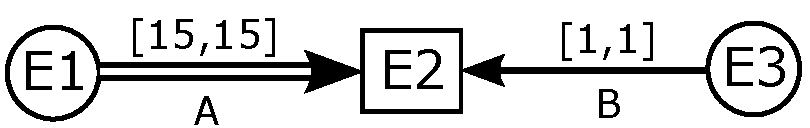
\includegraphics[width=0.6\textwidth]{figures/numerical_issues/num_1.pdf}
	\caption{The CCTPU with a relaxed lower bound for uncertain duration $A$}
	\label{fig:num_issue_1}
\end{figure}


\begin{figure}[htb]
	\centering
	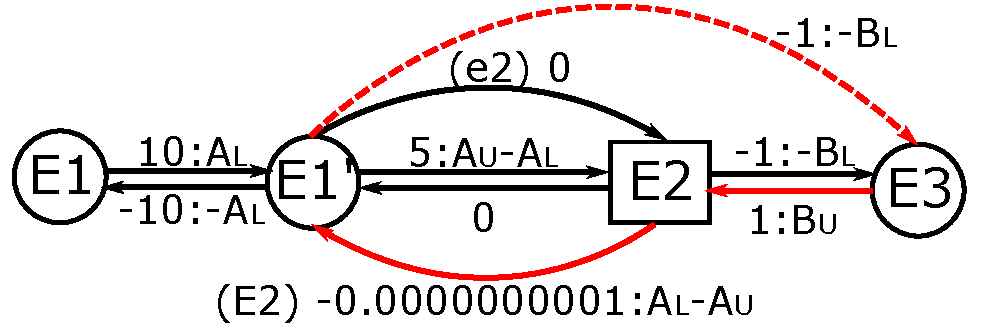
\includegraphics[width=0.6\textwidth]{figures/numerical_issues/num_2.pdf}
	\caption{The reduced graph with additional edges}
	\label{fig:num_issue_2}
\end{figure}


There are several options to resolve or reduce the chance of running into this
numerical issue: we may slightly relax the \textit{sensitivity} of the controllability
checker, set the continuous relaxation generator to \textit{over-relax} a bit, or
switch to rational numbers which eliminates the numerical issue
completely. We took the first approach since it provides the most intuitive
configuration and the flexibility to work in all situations: the over-relaxation
approach does not apply to problems whose solution space is very small, such as
the RCPSPs used by \citeA{cui2015optimising} in their experiments; the rational number approach requires an
approximation step to scale up the temporal bounds and rounding, whose impact
on the correctness of BCDR is difficult to estimate. As mentioned in earlier
sections, all temporal feasibility checking functions (consistency, strong controllability and
dynamic controllability) depend on a negative cycle detection function
implemented based on the Bellman-Ford algorithm, and the key in our approach is to
\textit{loosen} the criteria for a negative loop. Therefore, we modified the condition
for distance updates in Bellman-Ford, and the changes are highlighted in
Algorithm \ref{alg:modified_bellmanford}.


\begin{algorithm}[h!]
	
	\SetAlgoLined
	\SetKwFunction{Return}{return}
	\SetKwInput{Input}{Input}
	\SetKwInput{Output}{Output}
	\SetKwInput{Initialize}{Initialization}
	\SetKwInput{Algorithm}{Algorithm}
	\SetKwIF{If}{ElseIf}{Else}{if}{then}{else if}{else}{endif}
	\Indm
	\Input{\\
		$G$: $\langle V, E, s\rangle$, a weighted directed graph with vertices $V$, edges $E$ and source $s$;\\
	       $\epsilon$: the sensitivity settings for negative cycle detection.}
	\Output{$Cycle$: a collection of edges in $E$ that forms a negative cycle.}
	\Initialize{}
	\Indp{$Distance\leftarrow []$; the array for storing minimal distances from source to each vertex.}\;
	{$PredecessorEdge\leftarrow []$; the array for storing predecessor edge for each vertex}\;
	\Indm
	\Algorithm{}
	\nonl\textsc{RelaxedBellmanFord}($\mathit{G}$,$\mathit{\epsilon}$)\\
	\Indp
	// Initialize distance and predecessor array\;
	\nonl ... ...\\
	// Update distances from source to each vertex, only if the distance decreased by at least $\epsilon$\;
	\For{$i \in [1,\textsc{Length}(V)-1]$}{
		\For{$e \in E$}{
			\If{$Distance[\textsc{From}(e)] + \textsc{weight}(e) + \boldsymbol{\epsilon} < Distance[\textsc{To}(e)]$}{
				\nonl ... ...\\
			}
		}
	}
	// Extract negative cycle, if exists\;	
	\For{$e \in E$}{
		\If{$Distance[\textsc{From}(e)] + \textsc{weight}(e) + \boldsymbol{\epsilon} < Distance[\textsc{To}(e)]$}{
			\nonl ... ...\\
			\Return $Cycle$\;
		}
	}
	\Return null\;
\caption{Bellman-Ford algorithm with relaxed criteria on distance updates}
\label{alg:modified_bellmanford}
\end{algorithm}


There are three steps in the Bellman-Ford Algorithm: initialization of distance
and predecessor for vertices, updating the shortest distances to each vertex
from source, and detecting and extracting any negative cycles. The key
modification we made is the introduction of a non-negative sensitivity parameter
$\epsilon$, which is used during the updates of vertex distances (Line 7) and
the extraction of negative cycle (Line 13). It requires the new distance to be
$\epsilon$-less than the original distance, instead of just being smaller,
effectively making it more difficult for updates to take place. As a result, no
negative cycle with value larger than $-\epsilon$ in the original graph will be
detected, since such small differences will not be captured during the distance
updates. This parameter can be tuned for different applications to eliminate the
possibility of numerical issues while maintaining a good precision and
reliability. In our experiments, we set $\epsilon$ to $10^{-9}$ and found it to
be sufficient to completely eliminate the numerical issues.


\subsubsection{Delayed conflict resolutions}


Computing continuous relaxations is the most expensive procedure in BCDR. On the other hand, most of the
relaxation computation is not directly contributing to the final solution: we
compute relaxations to all known conflicts so that a new candidate can be generated
to help find new conflicts. For example, when solving a simple over-constrained
STN from the bus scheduling domain (discussed in the next section) with 417
events and 672 constraints, 381 continuous relaxation operations were executed
by BCDR in order to discover the 381 conflicts and find the optimal solution.
Out of the 17.01 seconds run-time, 13.14 seconds were consumed by computing continuous
relaxation, and the one we are mostly interested in is the last one when we have
learned all conflicts. The process is visualized in Figure
\ref{fig:conflict_resolution_time_1}, in which we plot the cumulated runtime
against the number of continuous conflicts discovered, and the continuous relaxation computation time against
the number of conflicts it is resolving. To improve the efficiency of this
procedure, the key is to discover new conflicts without incurring so many
expensive operations for computing optimal continuous relaxation, such
that the run time does not increase as fast when discovering new conflicts.


\begin{figure}[!ht]
	\centering
	\begin{subfigure}[b]{0.8\textwidth}
		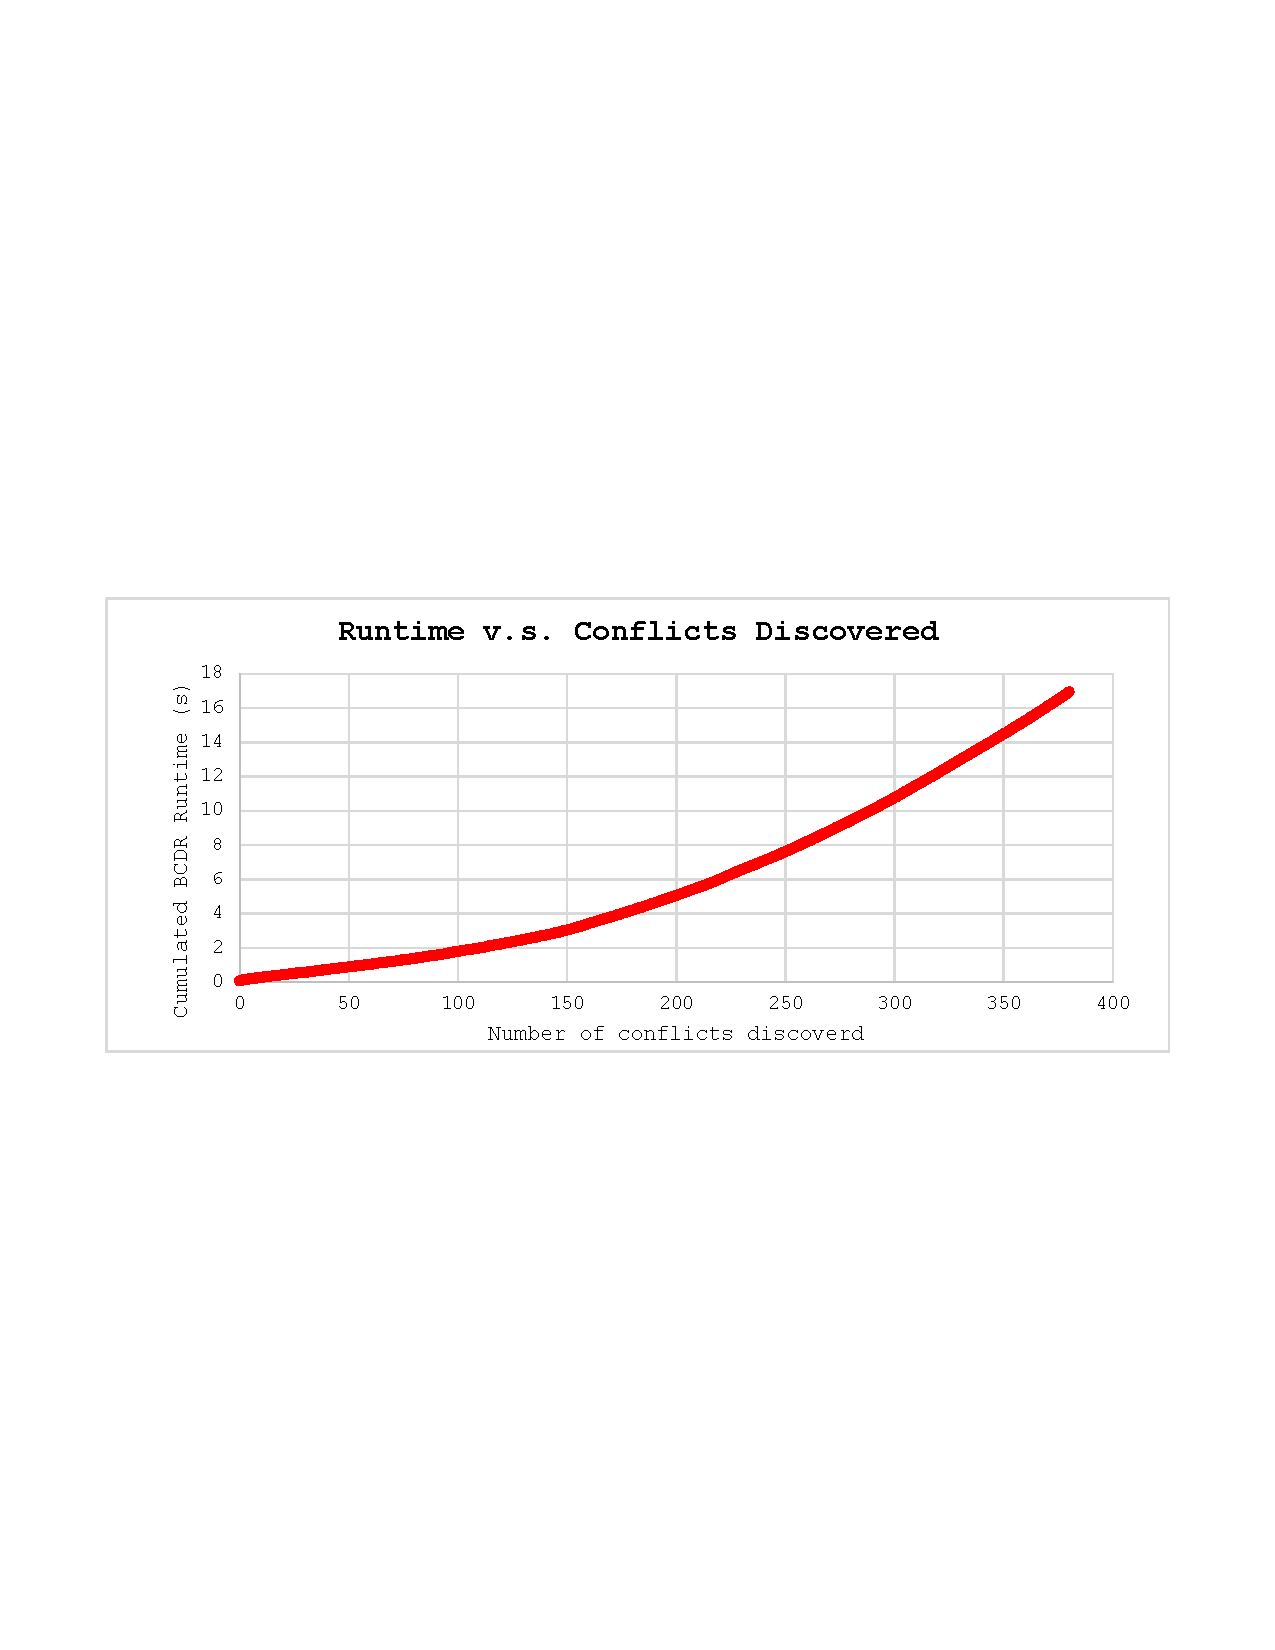
\includegraphics[width=\textwidth,trim={2.6cm 10.2cm 2.4cm 10.3cm},clip]{figures/BunchConflict/runtime_conflict_discovered_nobunch.pdf}
		\caption{}
		\label{fig:cumulatied_conflict_discovery}
	\end{subfigure}
	\begin{subfigure}[b]{0.8\textwidth}
		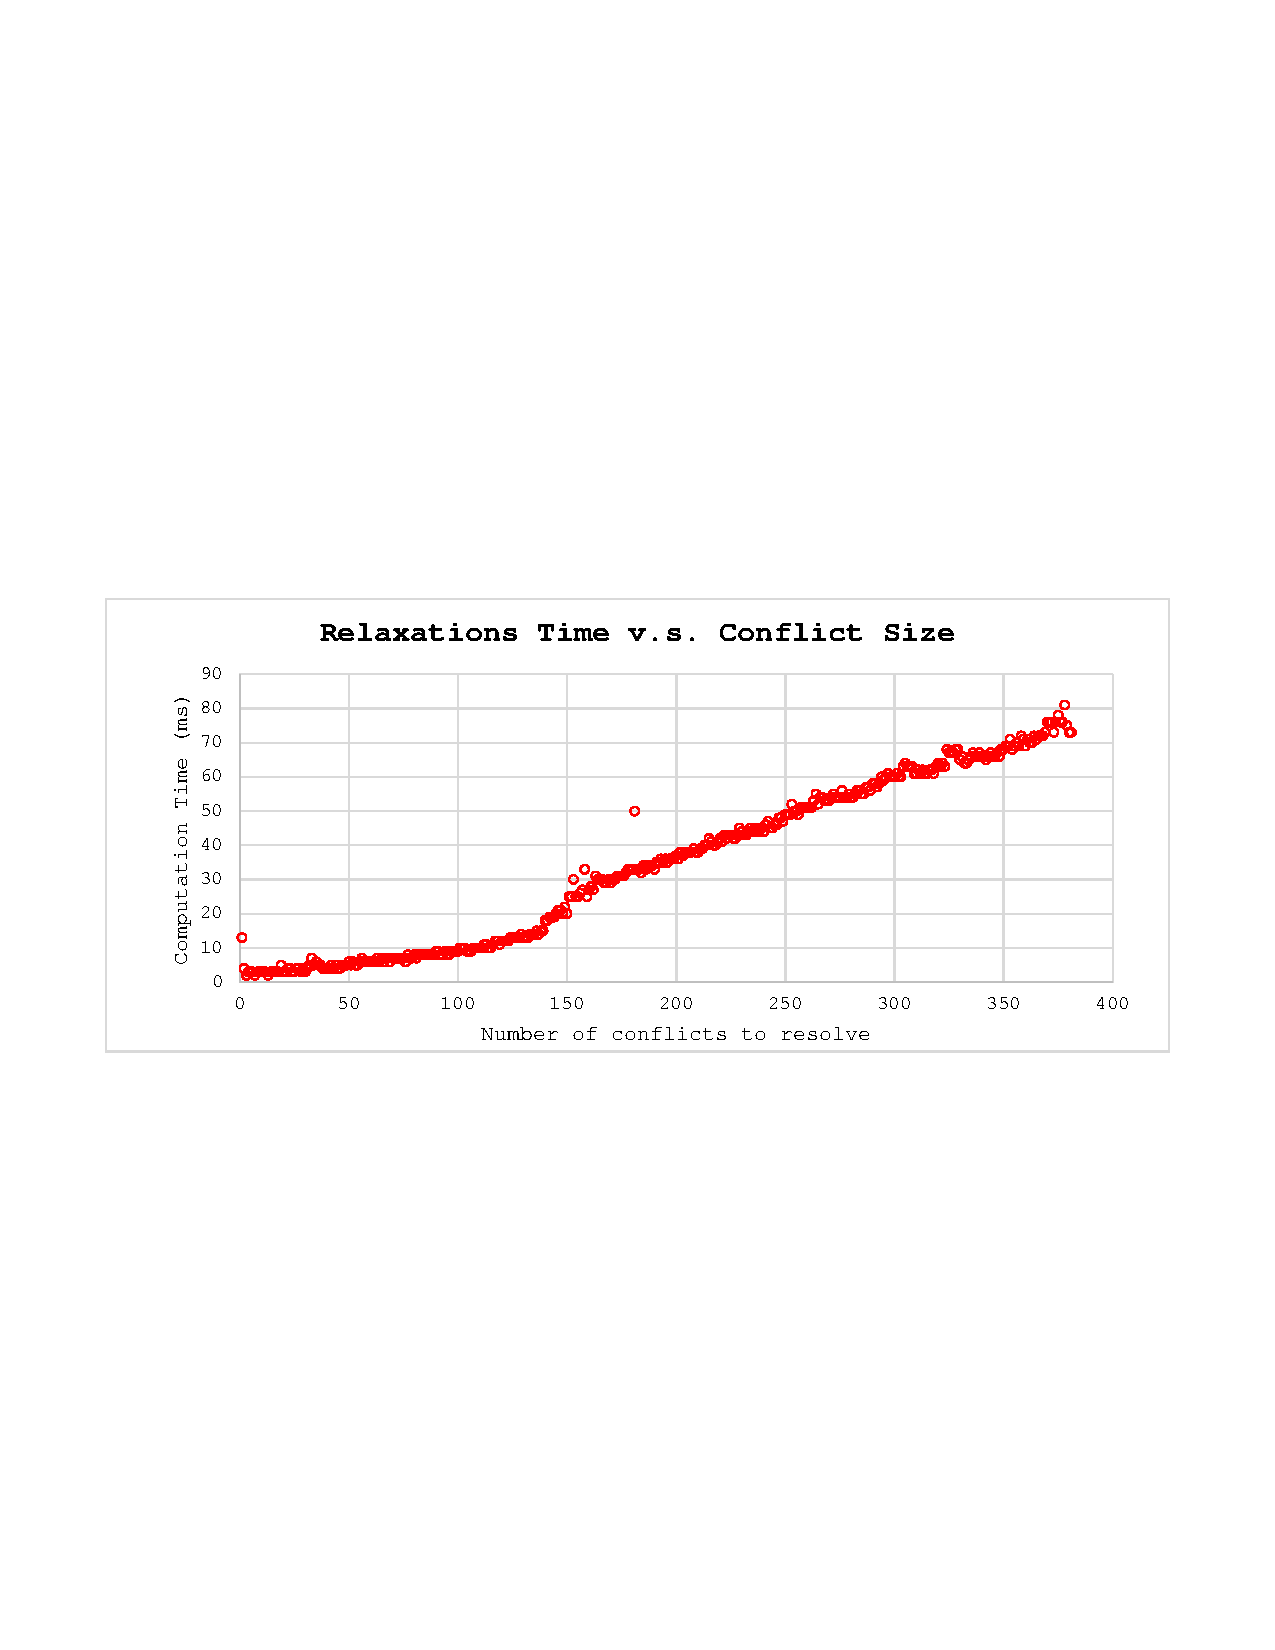
\includegraphics[width=\textwidth,trim={2.6cm 10.2cm 2.4cm 10.3cm},clip]{figures/BunchConflict/relaxation_time_nobunch.pdf}
		\caption{}
		\label{fig:cont_relaxation_time}
	\end{subfigure}
	\caption{Profile of Continuous Relaxations in BCDR Runtime}
	\label{fig:conflict_resolution_time_1}
\end{figure}


Therefore, we developed a greedy approach for resolving continuous conflicts during search:
picking the constraints with the lowest relaxation cost in a conflict, and
relaxing their lower or upper bounds to the extent that the linear expression of
the conflict is non-negative. The exact continuous relaxation procedure only
needs to be called to refine the relaxations when a consistent set is found:
during the search we may use the greedy approach for a new candidate that can
push BCDR to discover new conflicts. It takes very little time compared to the
exact optimal relaxation, since it does not require calling the optimizer. It
has significantly improved BCDR's runtime performance on large-scale and highly
constrained problems. For the same over-constrained problems, this greedy
relaxation approach reduces the runtime to 7.2 seconds, within which only 0.89
second were spent on conflict resolution. The same relaxation time and plot are
shown in Figure \ref{fig:conflict_resolution_time_improved}. Each point in
Figure \ref{fig:cont_relaxation_time_improved} represents the discovery of one
conflict. The closer it is to the x-axis, the less time was spent on computing
continuous relaxations after discovering the conflict. As can be seen in the
graph, less than ten exact relaxations were computed to refine the greedy
relaxations on this problem, which greatly reduces BCDR's run time: greedy
relaxations were used in most situations to discover new conflicts. The
downside is that we discovered more conflicts than before (566 vs 381), which
may not be necessary for generating the optimal relaxation.


\begin{figure}[!ht]
	\centering
	\begin{subfigure}[b]{0.8\textwidth}
		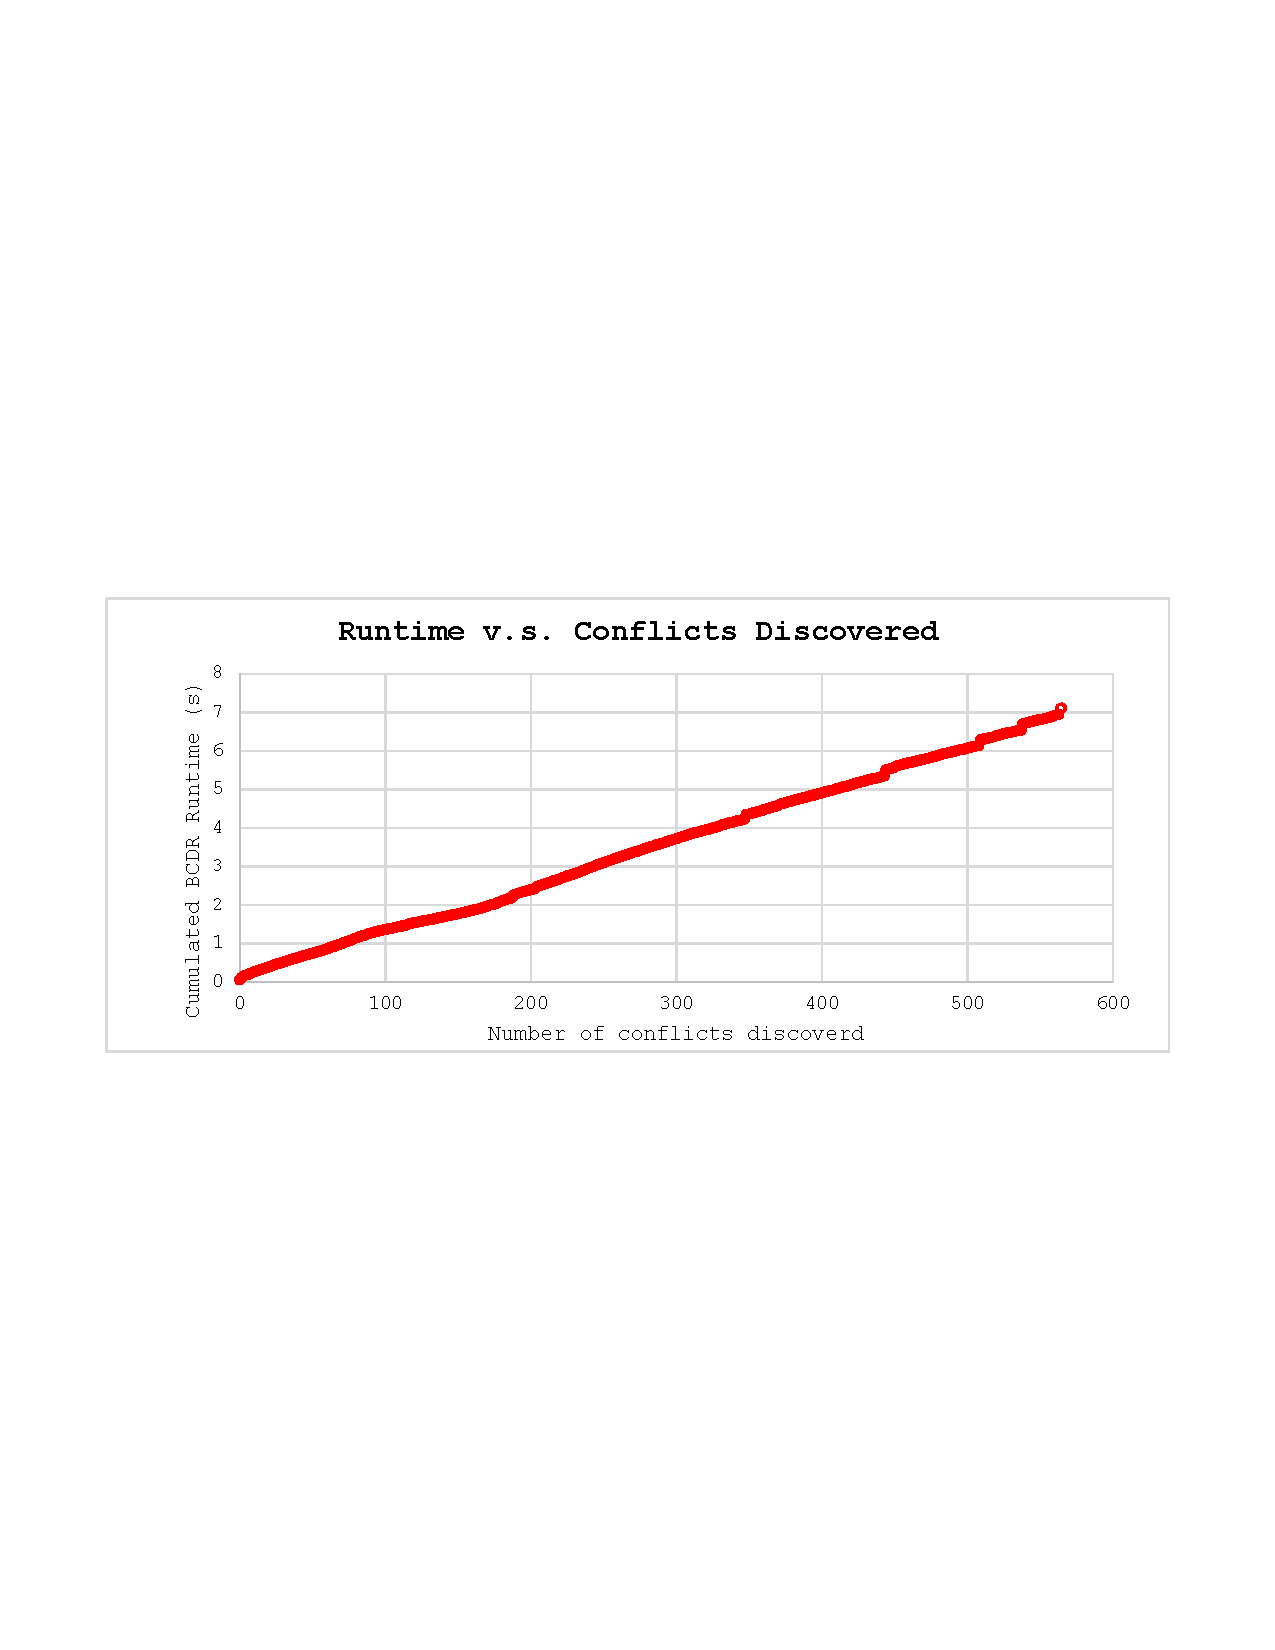
\includegraphics[width=\textwidth,trim={2.5cm 10.2cm 2.4cm 10.3cm},clip]{figures/BunchConflict/runtime_conflict_discovered_400bunch.pdf}
		\caption{}
		\label{fig:cumulatied_conflict_discovery_improved}
	\end{subfigure}
	\begin{subfigure}[b]{0.8\textwidth}
		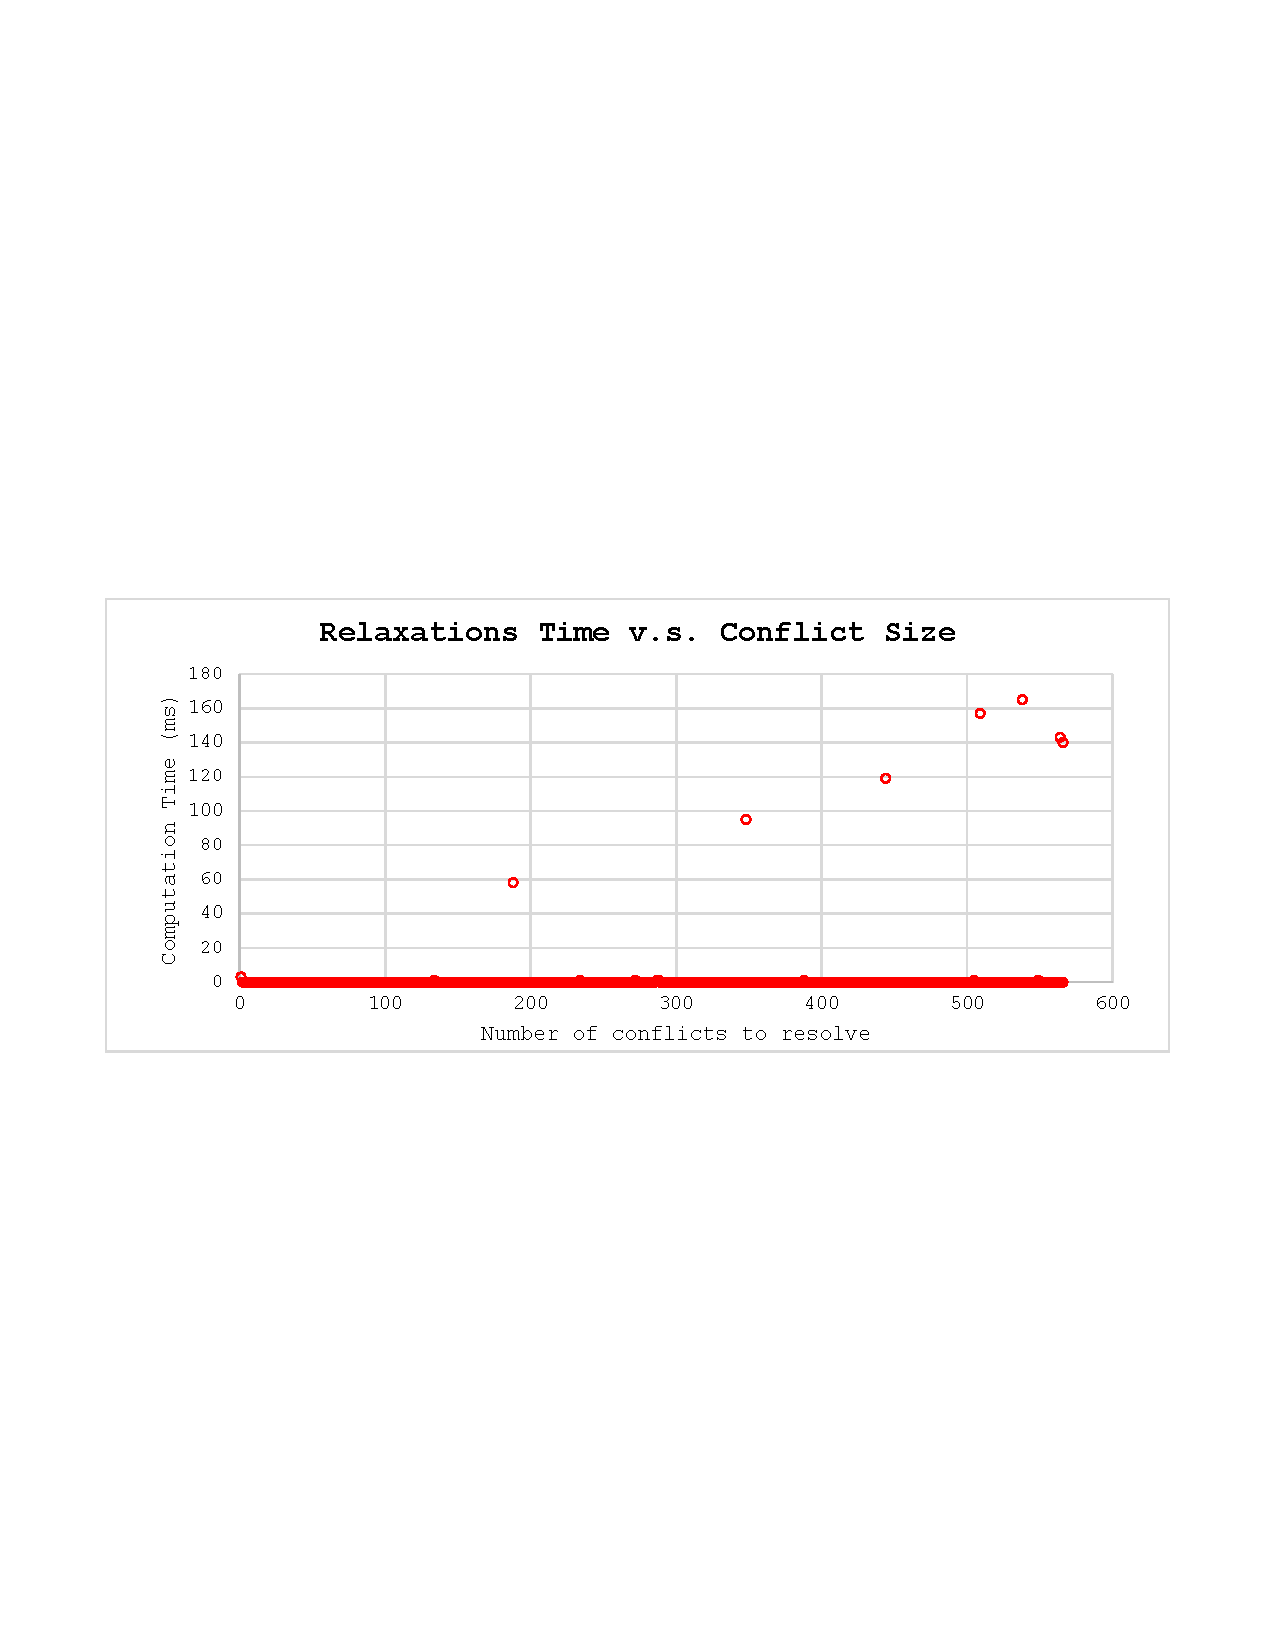
\includegraphics[width=\textwidth,trim={2.6cm 10.2cm 2.4cm 10.3cm},clip]{figures/BunchConflict/relaxation_time_400bunch.pdf}
		\caption{}
		\label{fig:cont_relaxation_time_improved}
	\end{subfigure}
	\caption{Profile of Combined Greedy/Exact Relaxations in BCDR Runtime}
	\label{fig:conflict_resolution_time_improved}
\end{figure}


The greedy approach requires very minimum modification to BCDR: instead of
formulating and solving the optimization problem in \textsc{ExpandOnConflict}, we compute the greedy relaxations here. Inside
\textsc{ExpandOnConflict}, Line 16 to Line 22 (Algorithm \ref{alg:ExpandOnConflict}) are replaced with a new procedure
that only looks at the new conflict $\mathit{currConf}$  (Algorithm \ref{alg:ExpandOnConflict_greedy}), instead of all conflicts that
were previously resolved continuously. The
greedy relaxation procedure iterates through all constraints in the conflict
and checks if any constraints involved are relaxable (Line 16-17). If such a
constraint is identified, it will relax its bounds, either lower or upper, to
the maximum extent or to the extent that the conflict is eliminated, whichever
is smaller (Line 18). The initial value of the conflict's linear expression is
captured by the variable $\mathit{Offset}$, and the conflict is resolved once the
variable is made zero or negative. If one constraint cannot provide enough
deviation, the procedure will move on to the next one, until $\mathit{Offset}$ is made
zero or less. If the loop completes but the offset is still positive, it means
that no continuous relaxation is available for resolving the new conflict, and
the continuous relaxation candidate will not be generated.


\begin{algorithm}[htb!]
	\setcounter{AlgoLine}{15}
	\nonl ... ...\\
	\nonl \textbf{Initialize}\\
	\nonl {$\mathit{Offset}\leftarrow$ 0 - \textsc{EvalExp($\mathit{currConf}$)}};  amount of relaxation that need to be applied for resolving the conflict continuously\;
	\nonl ... ...\\
	\For{$c \in \mathit{currConf}$}{
		\If{\textsc{isRelaxable($c$)}}{
			$r = \textsc{Min}(\mathit{Offset},\textsc{RelaxationLimit}(c))$\;
			$R_{new} \leftarrow R_{new} \cup \{\langle c,\textsc{LB}(c)-r,0\rangle \}$ or $\{\langle c,0,\textsc{UB}(c)+r\rangle \}$\;	
			$\mathit{Offset} = \mathit{Offset} - r$\;
		}
		\If{\textsc{$\mathit{Offset} \leq 0$}}{
			$\mathit{Cand_{new}}\leftarrow\langle A,R_{new},C_r,C_{cont}\rangle $\;
			$\mathit{newCands}\leftarrow \mathit{newCands}\cup \mathit{Cand_{new}}$\;
			break;
		}
	}
	\nonl ... ...\\
	\caption{Modifications to Function \textsc{ExpandOnConflict} (Algorithm \ref{alg:ExpandOnConflict}) for handling candidates with greedy relaxation}
	\label{alg:ExpandOnConflict_greedy}
\end{algorithm}


The optimal relaxation procedure is moved outside of \textsc{ExpandOnConflict}, and to the main loop of BCDR. Once BCDR has verified
the feasibility of a candidate solution, instead of retuning it, an additional
procedure will be executed to check if the candidate contains any greedy
relaxations (Line 12, Algorithm \ref{alg:bcdr_greedy}). If true, it will refine
the relaxations using the optimization procedure and generate a new candidate.
The new candidate will be put back to the queue for further verification, since
it may not be the best or consistent candidate after the updates to its
continuous relaxation. The greedy approach always underestimates the cost of resolving conflicts, ensuring that the heuristic function of BCDR remains admissible. This refinement step corrects such underestimation before returning candidates,  allowing BCDR to enumerate resolutions in best-first order with delayed conflict resolution.



\begin{algorithm}[htb!]
\setcounter{AlgoLine}{9}
\nonl ... ...\\
$\mathit{newConf}\leftarrow$\textsc{ConsistencyCheck}$(\mathit{Cand})$\;
\If{$\mathit{newConf}==null$}{
	\eIf{\textsc{HasGreedyRelaxation}($cand$)}{
		$cand_{opt} \leftarrow$ \textsc{RefineRelaxation}($\mathit{Cand}$)\;
		$Q\leftarrow Q\cup \{cand_{opt}\}$\;
	}{
		\Return $\mathit{Cand}$\;
	}	
}
\nonl ... ... \\
\caption{Modifications to the BCDR algorithm (Algorithm \ref{alg:bcdr}) for greedy continuous relaxation}
\label{alg:bcdr_greedy}
\end{algorithm}



This approach works very well on non-conditional problems, whose search tree has
one single branch. However, it may not save time on conditional ones. To enumerate candidate solutions in best-first order, BCDR needs an
accurate estimation for the cost of relaxation in order to prioritize
candidates. In order to keep the heuristic function admissible, the cost for all
greedy relaxation are set to zero. This is because the greedy relaxations will
all have larger than optimal cost, and we have no idea how much the `minimal cost'
will be. Hence, setting the cost to be zero retains the admissible property and
still allows BCDR to do a best-first enumeration. However, if we stick to the
greedy relaxations, the utility estimation for candidates may be off by a large
margin, causing BCDR to waste a lot of time examining candidate solutions that
are far from the optimal.


Therefore, we propose a mixed greedy-optimal relaxation approach to achieve a
good balance between efficiency and accuracy. The new approach uses greedy
relaxation when more conflicts are likely to be discovered, and only runs the
continuous relaxation procedure if we are confident that no more conflicts will be
discovered, or we have been applying greedy relaxation for more than $N$ times
consecutively. If a candidate is found to be consistent, or has more than $N$
greedy relaxations, the exact relaxation procedure will be used. The parameter
$N$ is a non-negative integer, and if $N$ is too large then the utility
estimation may be off by too much. Therefore, in our experiments we have been
using $N=5$ to achieve a good balance between the time saving and the risk of
creating a huge difference in heuristic and actual costs.



\section{Applications and Empirical Evaluation}


In this section, we discuss the three applications of BCDR, in the domains of
deep-sea mission planning, transit vehicle scheduling, and resource-constrained
project scheduling. Within each of the applications, we present the modeling of
the problems, the configurations of BCDR for solving them, and the experiments
for evaluating BCDR's performance compared to alternative approaches or
commercial solvers. These problems are of very different structure and scale,
and through these experiments, we tried to explore the strength and weakness of
BCDR. Our Python implementation of BCDR used in these experiments, along with
all the test cases created, can be found on GitHub: https://github.com/yu-peng/cdru.


All experiments presented in this section were conducted on a desktop computer
with an Intel Core i5-3470 processor and 16GB of RAM. The SNOPT optimizer we used
is version 7.2, and the Gurobi optimizer is version 6.5.1.


\subsection{Managing Deep-sea Exploration Missions}


As presented in the beginning of the paper, the BCDR algorithm has been
incorporated as part of a mission advisory system for helping ocean scientists
schedule autonomous underwater vehicle tasks in deep-sea expeditions. Their
missions are usually weeks long, and involve the operations of several
AUVs. Each vehicle usually performs ten to fifteen dives in a
mission, and a dive may last between 6 to 16 hours. During each dive, a
vehicle is tasked with a set of survey locations on the sea floor: the vehicle needs
to traverse between each location, take samples and images, and return before running
out of power. Due to unexpected ocean currents and incomplete terrain data, the
traversal time between survey sites is highly uncertain and difficult to
estimate. It is almost impossible for the scientists to correctly assess the
uncertainty of each dive and plan tasks accordingly to meet the risk bound and a
large set of operational constraints.


The advisor can check the feasibility
of a mission plan and search for valid risk allocations that meet the risk
requirement. If no such allocation can be found, the decision aid will explain
the cause of failure using the conflicts detected during the search, and propose
preferred relaxations to resolve the over-constrained plan. If the users are not
satisfied with the results, they can ask the mission advisor to adjust the
solutions given their new inputs. 


We examined the performance of BCDR on problems generated from this domain, with
different sizes and complexity. The test cases were created using a mission
simulator for underwater expeditions. Given a set of target locations on a map,
the simulator generates survey tasks around them and connects these locations
with traversal activities. Each test case describes the operations of multiple
AUVs over several dives, and each vehicle's dive may contain multiple survey
tasks. In addition, the traversals are represented by probabilistic durations,
while the survey times and battery restrictions are modeled by simple temporal
constraints. The operational risk limit is specified by the chance constraints
in the cc-pCCTPs. Multiple underwater robots may be deployed and working in
parallel during a dive: each robot may have different speed and power storage.
Depending on the distance and vehicles, probabilistic durations of different
traversals and robots have different distributions.


These test problems have a very unique \textit{relay} type structure: resources
are being used repeatedly for different tasks, with constraints restricting the
start times, end times or durations of the tasks. In addition to deep-sea
exploration, this structure is also shared by problems in many other domains,
such as scheduling vehicle usage in a car-sharing network.


\subsubsection{Setup}


The randomly generated mission cc-pCCTPs have a similar structure to the example
presented in Section 2. To make it more complex, we extended the problems to
include multiple robots and dives: there is always another scientist waiting for
the shared robot following each dive; and there are multiple robots that are
operating in parallel. We use the following control parameters in the mission
problem generator to characterize the complexity of a test case:


\begin{itemize}
	\item $N_d$: number of dives per robot. $1\leq N_d\leq 5$.
	\item $N_r$: number of AUVs available. $1\leq N_r\leq 12$.
	\item $N_{act}$: number of activities per dive. $1\leq N_{act}\leq 4$.
	\item $N_{opt}$: number of alternatives per activity. $2\leq N_{opt}\leq 6$.
\end{itemize}


The total number of discrete variables in a test case is $N_d\times N_r\times
N_{act}$, and the domain size of each variable is determined by its $N_{opt}$.
Each problem is constructed as follows. We randomly sample locations from a
region in Northern Pacific, within a 10km radius of (33.251, -121.555). The
traversal times are computed using an average speed randomly selected between 10
and 20 kilometers per hour. The survey length at each location and the dive
duration, $T_{act}$ and $T_{div}$, are randomly sampled in $[10,90]$ and
$[60,960]$ (minutes), respectively. These durations are encoded as relaxable
temporal constraints. We define linear preference functions over these relaxable
constraints with gradient (cost per minute) sampled between 0 and 10. The reward
for each variable assignment, denoting a location selection for each survey
activity, ranges from 0 to 1000. For example, Figure \ref{fig:test_case_auv}
presents an overview for the structure of a test case with 2 vehicles and each
carries our two activities during their dives.


\begin{figure}[htb]
	\centering
	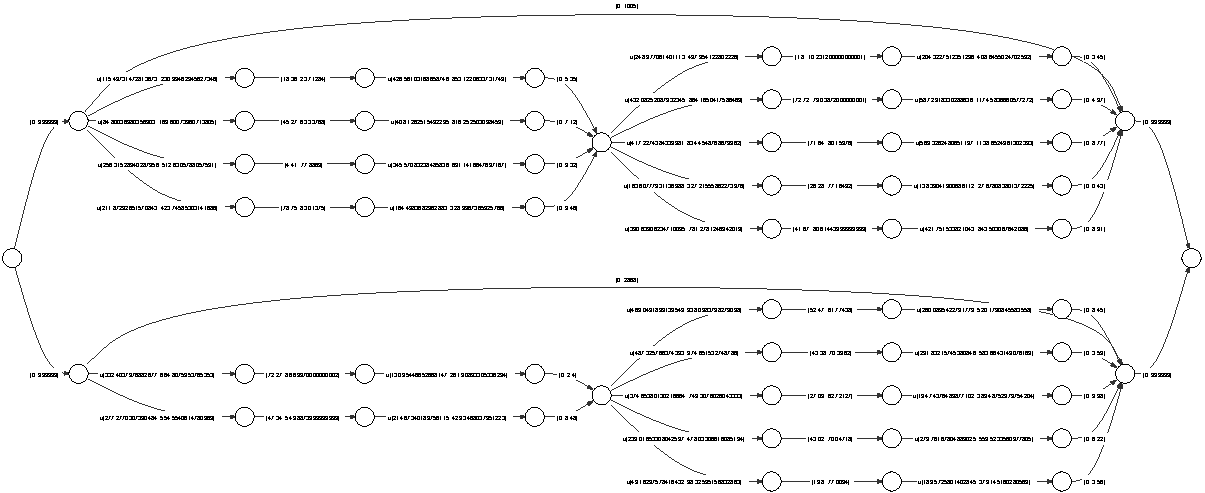
\includegraphics[width=1.0\textwidth]{figures/test_case_auv.pdf}
	\caption{Overview of the structure for a test case}
	\label{fig:test_case_auv}
\end{figure}


In total, we created 2400 test cases using randomly generated numbers of robots,
risk bounds, survey locations and mission length. For each test case, we run
BCDR with the following five configurations:


\begin{enumerate}[A.]
	\item Consistency: determine and restore the feasibility of the test cases
	using BCDR. This algorithm is denoted as `BCDR'. The cc-pCCTPs are treated as
	CCTPs by this configuration: the uncertain durations are assigned lower and
	upper bounds equal to their mean $[\mu, \mu]$.
	
	\item Strong Controllability: using BCDR-U with a strong controllability model
	to determine and restore the feasibility of the test cases. This algorithm is
	denoted as `BCDR-U(SC)'. The cc-pCCTPs are treated as CCTPUs: the uncertain
	durations are assigned lower and upper bounds computed from their mean and
	variance $[\mu-3\sigma, \mu+3\sigma]$.
	
	\item Dynamic Controllability: using BCDR-U with a dynamic controllability
	model to determine and restore the feasibility of the test cases. This
	algorithm is denoted as `BCDR-U(DC)'. The cc-pCCTPs are treated as CCTPUs: the
	uncertain durations are assigned lower and upper bounds computed from their
	mean and variance $[\mu-3\sigma, \mu+3\sigma]$.
	
	\item Chance-constrained Strong Controllability: using BCDR-C to find a
	grounded STNU of the cc-pCCTP that is strongly controllable while meeting the
	chance constraint, or a set of relaxations for the cc-pCCTPs that will enable
	such a STNU. This algorithm is denoted as `BCDR-C(SC)'.
	
	\item Chance-constrained Dynamic Controllability: using BCDR-C to find a
	grounded STNU of the cc-pCCTP that is dynamically controllable while meeting the
	chance constraint, or a set of relaxations for the cc-pCCTP that will enable
	such a STNU. This algorithm is denoted as `BCDR-C(DC)'.
\end{enumerate}





\subsubsection{Results}


In this experiment, we benchmarked BCDR and its variants on each problem using
the five aforementioned configurations. We use SNOPT as the linear optimizer for
consistency and controllability based tests, and non-linear optimizer for
chance-constrained tests with probabilistic durations. In each test run, the
time consumption until the first solution returned, numbers of conflicts
detected, as well as the utility of the solution, were recorded. The timeout for
each run was set to be 30 seconds, which is usually the maximum duration
scientists are willing to wait for.


First, we present the results for Configuration A, B and C, which are BCDR,
BCDR-U(SC) and BCDR-U(DC). The runtime performance of the three algorithms are
presented in Figure \ref{fig:bcdr_runtime_results}. Each dot in the graphs
represents the cumulative number of instances solved on problems that contains
equal or less number of constraints, which are indicated by the x-axis. In
total, BCDR with temporal consistency checker solves 1589 problems within 30
seconds, while the number for BCDR-U(SC) and BCDR-U(DC) are only 430 and 695,
respectively. As can be seen from the figures, BCDR with consistency assumption
is able to solve problems with up to 1000 constraints, while the other two
algorithms never succeeded with problems beyond 500 constraints. This is the
result of the different handling of uncertain durations: due to the
consideration of all possible outcomes from each uncertain duration, both
controllability-based BCDR-U algorithms are more restrictive compared to the
consistency-based BCDR, which treats uncertain durations as controllable and may
only satisfy one of its many outcomes. Hence the number of conflicts detected
and resolved by both BCDR-U(SC) and BCDR-U(DC) are much higher than that of BCDR
(Figure \ref{fig:bcdr_conflicts_results}, \ref{fig:bcdr_sc_conflicts_results}
and \ref{fig:bcdr_dc_conflicts_results}), which significantly impacts their
performance on large problems.


\begin{figure}[!ht]
	\centering
	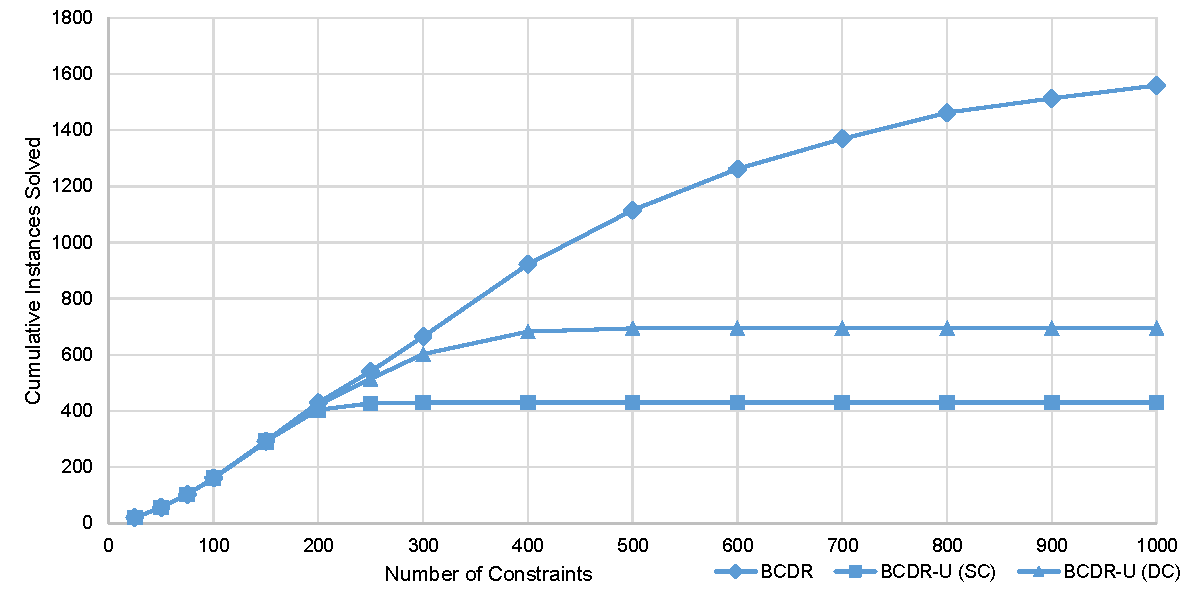
\includegraphics[width=0.9\textwidth]{figures/results/bcdr_runtime.pdf}
	\caption{Cumulative number of instances solved by BCDR (in 30 seconds)}
	\label{fig:bcdr_runtime_results}
\end{figure}


%\begin{figure}[!ht]
%	\centering
%	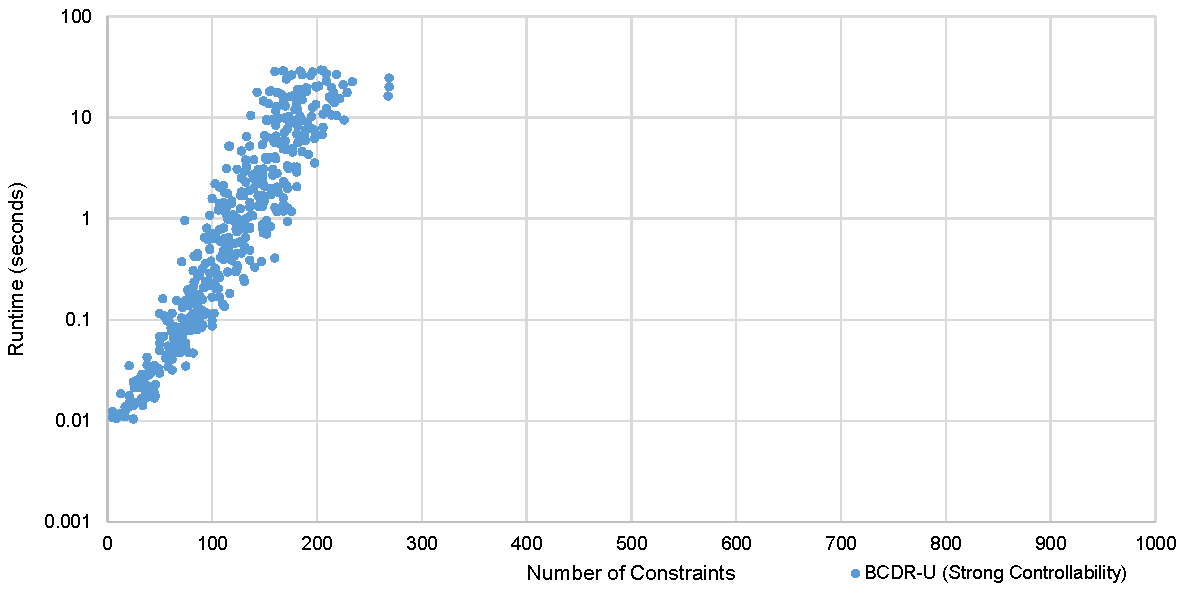
\includegraphics[width=0.9\textwidth]{figures/results/bcdr_sc_runtime.pdf}
%	\caption{Runtime of BCDR-U(SC)}
%	\label{fig:bcdr_sc_runtime_results}
%\end{figure}
%
%
%\begin{figure}[!ht]
%	\centering
%	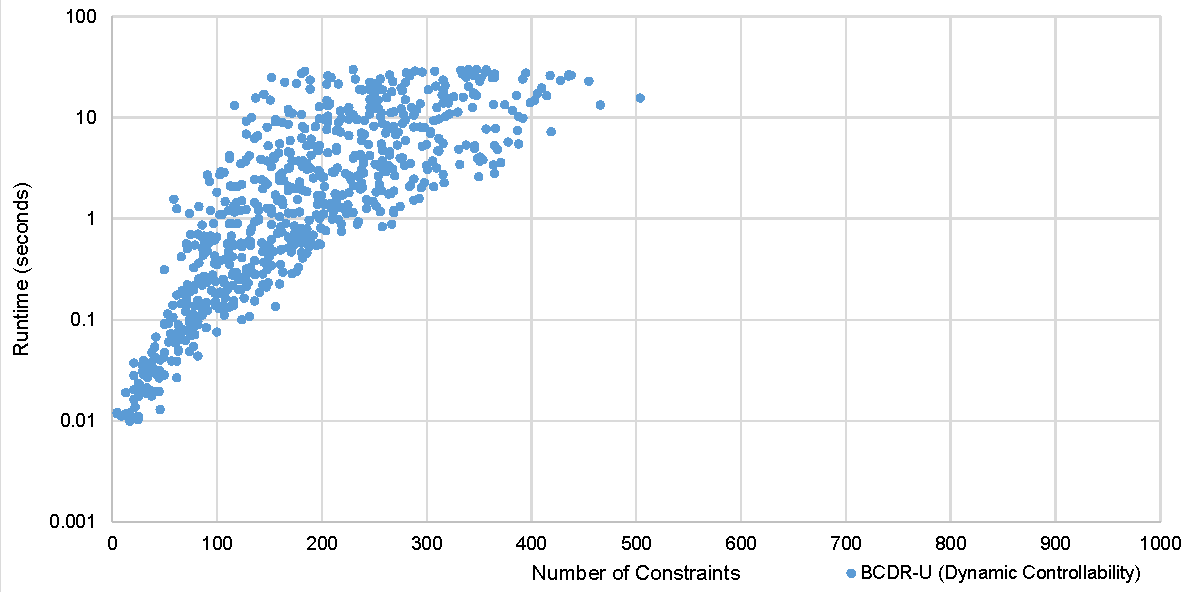
\includegraphics[width=0.9\textwidth]{figures/results/bcdr_dc_runtime.pdf}
%	\caption{Runtime of BCDR-U(DC)}
%	\label{fig:bcdr_dc_runtime_results}
%\end{figure} 


In addition, checking strong and dynamic controllability are also more expensive
operations than checking consistency, which contributed to their lower runtime
performance. As presented in Section 3, we use the Bellman-Ford algorithm for
consistency checking and negative loop extraction ($O(N^2logN)$). We add another
layer of triangular reduction ($O(N^2)$) on top of it for checking strong
controllability. For dynamic controllability, we use the \textsc{fastDCCheck}
algorithm $O(N^4)$, introduced by \citeA{Morris_astructural}. It is interesting to observe
that BCDR-U(DC) out-performs BCDR-U(SC), as there is an order-of-magnitude difference in their checking
algorithms' runtime complexity. This is likely the result of the smaller amount
of conflicts that were resolved by the dynamic controllability version, as shown
in Figure \ref{fig:bcdr_sc_conflicts_results} and
\ref{fig:bcdr_dc_conflicts_results}. Dynamic controllability allows more
flexibility than strong controllability in that it does not require a static
schedule to accommodate all constraints and uncertain durations. The runtime of
BCDR-U is dominated by conflict resolution for over-constrained problems, hence
the less time spent on conflict resolution compensated for the additional time
on controllability checking.


\begin{figure}[!ht]
	\centering
	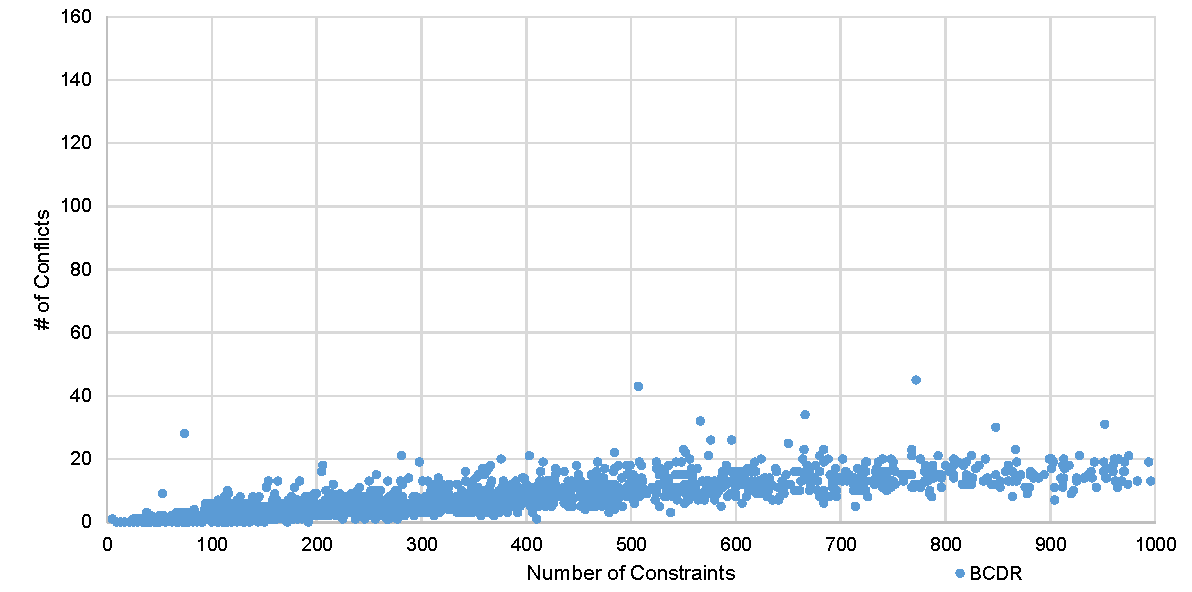
\includegraphics[width=0.9\textwidth]{figures/results/bcdr_c_conflicts.pdf}
	\caption{Conflicts detected by BCDR (Consistency)}
	\label{fig:bcdr_conflicts_results}
\end{figure}

\begin{figure}[!ht]
	\centering
	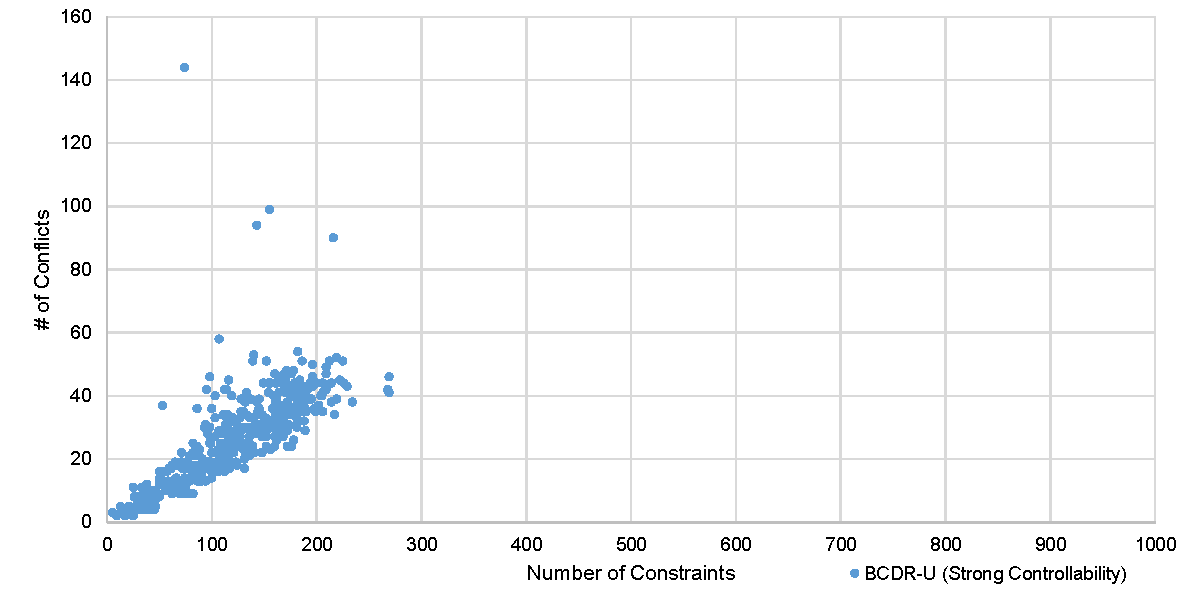
\includegraphics[width=0.9\textwidth]{figures/results/bcdr_sc_conflicts.pdf}
	\caption{Conflicts detected by BCDR-U(SC)}
	\label{fig:bcdr_sc_conflicts_results}
\end{figure}

\begin{figure}[!ht]
	\centering
	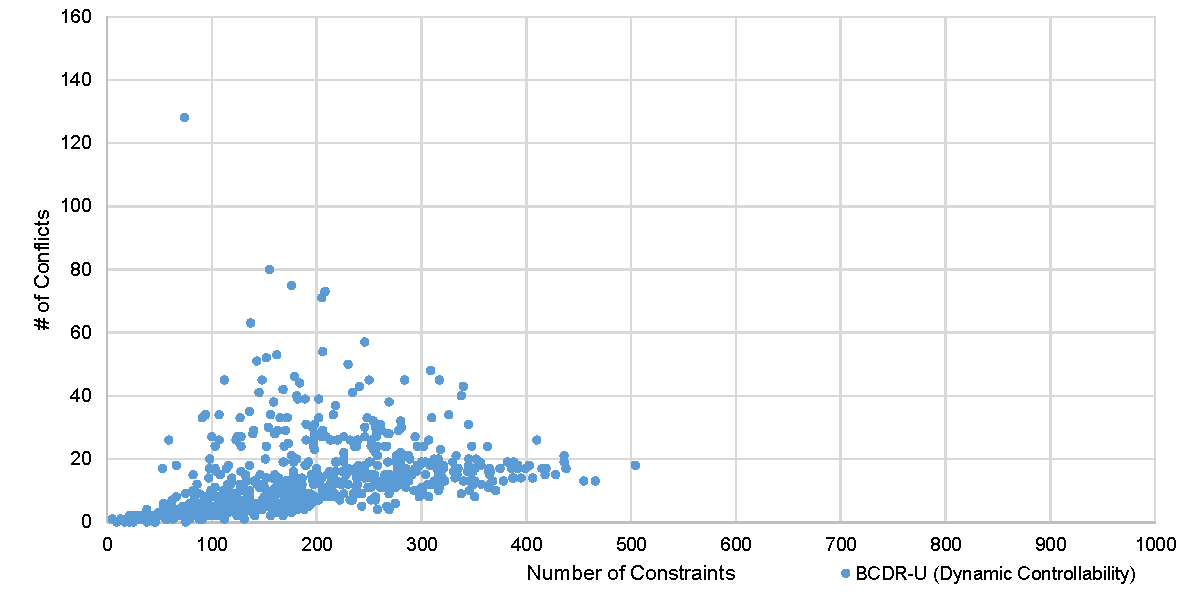
\includegraphics[width=0.9\textwidth]{figures/results/bcdr_dc_conflicts.pdf}
	\caption{Conflicts detected by BCDR-U(DC)}
	\label{fig:bcdr_dc_conflicts_results}
\end{figure}


%The different level of flexibility allowed by the three checking algorithms also
%affects the utility of the best solutions generated. We collected the 420 test
%problems that were solved by all three configurations, and evaluated the
%utilities of the best solutions returned by them. The results are shown in
%Figure \ref{fig:bcdr_utility_results}. For easier comparison, we present the
%results using two differences between the solution utilities: BCDR over BCDR-U(SC) and BCDR-U(DC) over BCDR-U(SC). The utility of BCDR-U(SC)
%solutions is set to zero as the baseline for comparison.
%
%
%\begin{figure}[!ht]
%	\centering
%	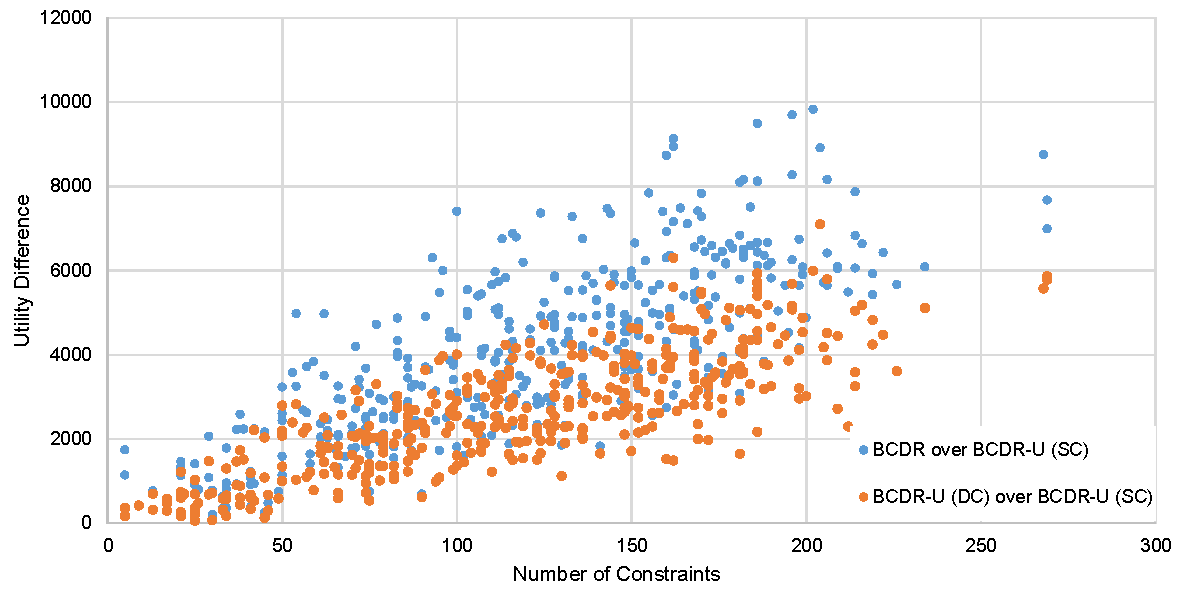
\includegraphics[width=0.9\textwidth]{figures/results/bcdr_utility.pdf}
%	\caption{Difference between solution utilities of BCDR, BCDR-U(SC) and BCDR-U(DC)}
%	\label{fig:bcdr_utility_results}
%\end{figure}
%
%
%The solutions generated by BCDR using the consistency checker have the highest
%utility, followed by BCDR-U(DC). The solutions generated
%by BCDR-U(SC) have the lowest average utility. In order to
%satisfy the uncontrollable outcomes of uncertain durations and restore the
%controllability of over-constrained temporal problems, BCDR-U adds or tightens constraints
%during the controllability checking process. Hence they have a more restricted
%solution space when compared to BCDR. As a result, their best solutions are
%usually of lower utility. As stated earlier, due to the less conservative
%execution strategy of dynamic controllability, BCDR-U(DC) imposes less
%constraints than BCDR-U(SC) and allows larger solution space. This can be
%measured by the number of conflicts detected and resolved by each algorithm
%before returning the solution (Figure \ref{fig:bcdr_utility_results}). The
%number of conflicts determines how constrained the optimization problem is while
%computing continuous relaxations: the more conflicts need to be resolved, the
%more constraints in the optimization, which require more relaxations to satisfy.
%This is why the solutions of BCDR-U(SC) are of lower quality: on average, it
%has to resolve two to three times more conflicts than BCDR-U(DC) before
%returning the best solution.
 

Next, we discuss the results of BCDR-C(SC) and BCDR-C(DC) (Configuration D and
E), the two chance-constrained relaxation algorithms with strong and dynamic
controllability checker. They were used to restore the feasibility of cc-pCCTPs
through both temporal and chance constraints relaxations. The results is shown
in Figure \ref{fig:bcdr_c_runtime_results}.


\begin{figure}[!ht]
	\centering
	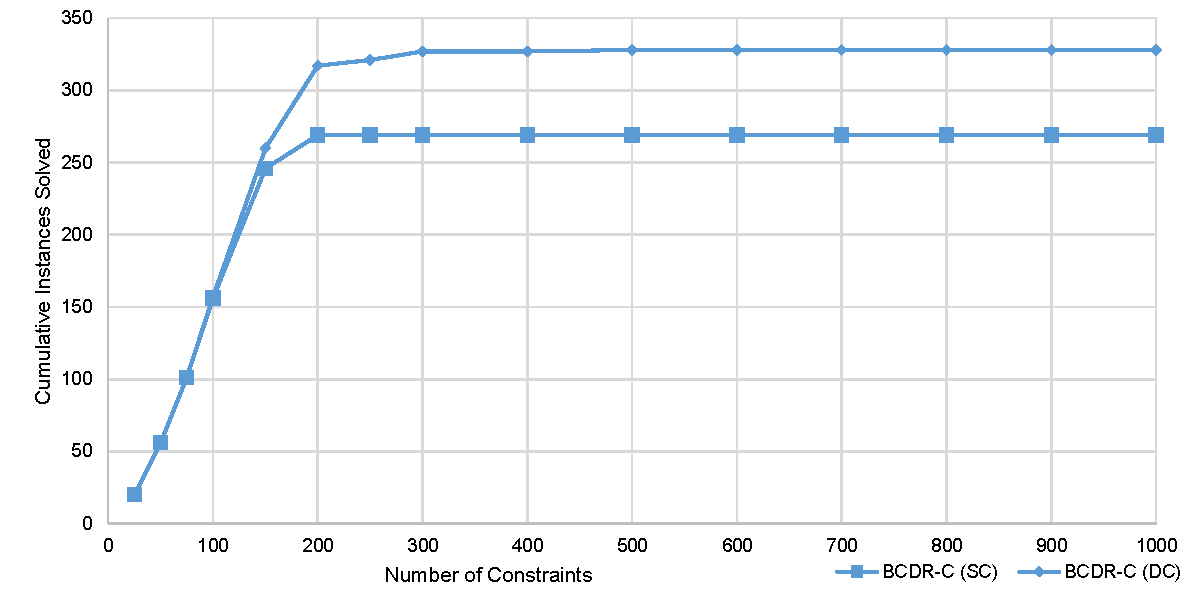
\includegraphics[width=0.9\textwidth]{figures/results/bcdr_c_runtime.pdf}
	\caption{Cumulative number of instances solved by BCDR-C (in 30 seconds)}
	\label{fig:bcdr_c_runtime_results}
\end{figure}


%\begin{figure}[!ht]
%	\centering
%	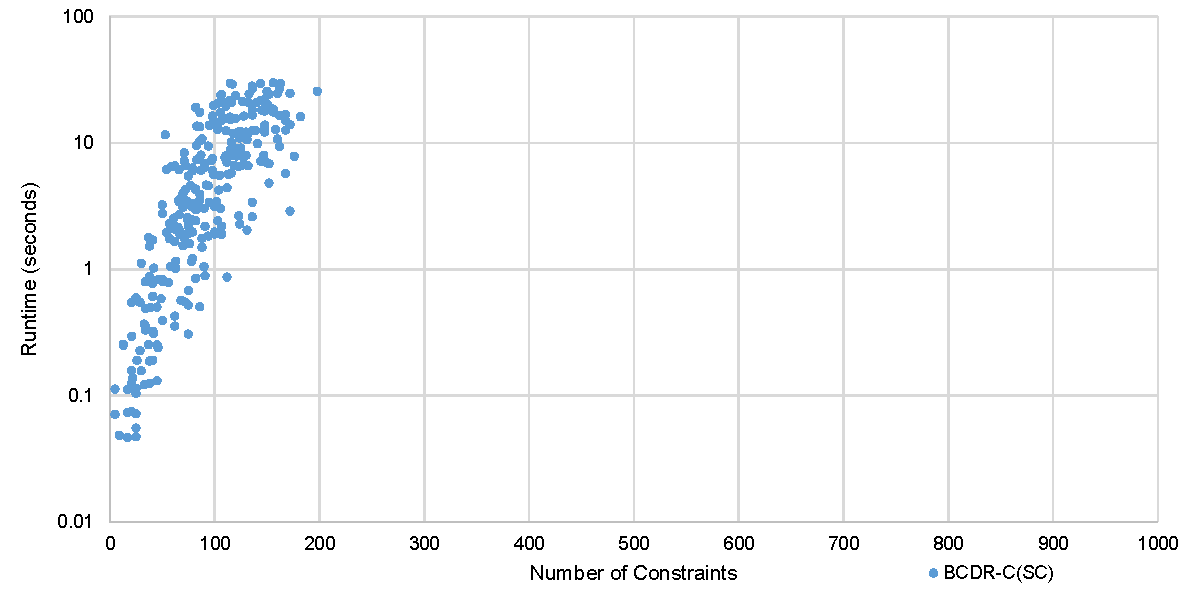
\includegraphics[width=0.9\textwidth]{figures/results/bcdr_cc_sc_runtime.pdf}
%	\caption{Runtime of BCDR-C(SC)}
%	\label{fig:bcdrc_sc_runtime_results}
%\end{figure}
%
%
%\begin{figure}[!ht]
%	\centering
%	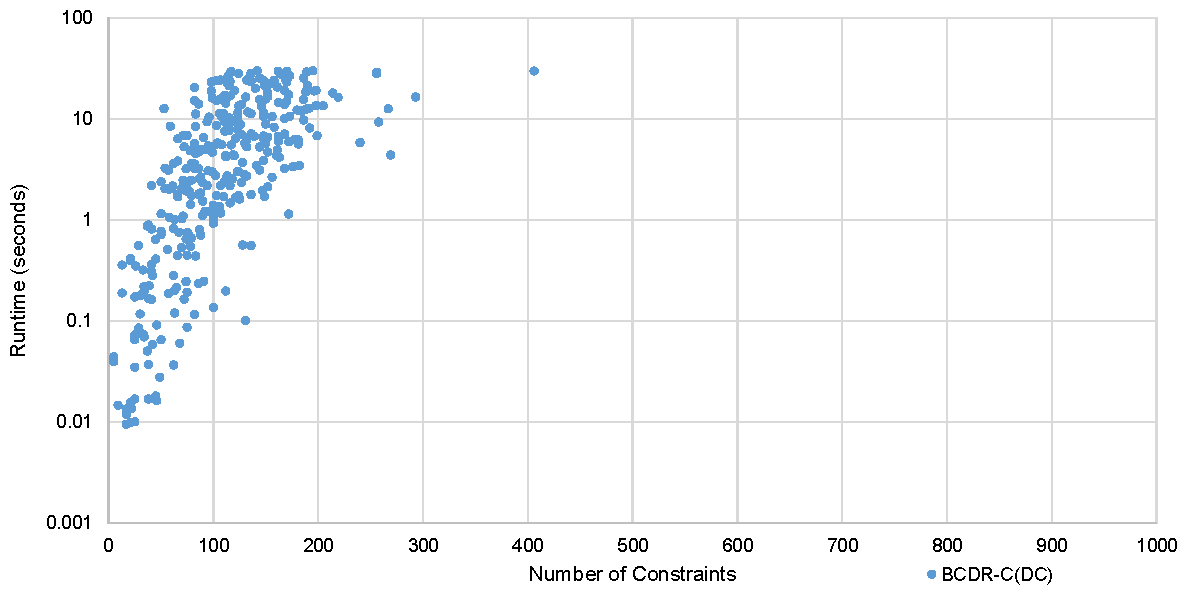
\includegraphics[width=0.9\textwidth]{figures/results/bcdr_cc_dc_runtime.pdf}
%	\caption{Runtime of BCDR-C(DC)}
%	\label{fig:bcdrc_dc_runtime_results}
%\end{figure}


In total, 269 of 2400 tests were solved by BCDR-C(SC) in 30 seconds, while the
number for BCDR-C(DC) is 328 of 2400. Similar to the BCDR-U experiment, the
dynamic controllability version performs better than the strong controllability
version due to the smaller number of conflicts. BCDR-C solves fewer problems than BCDR-U and BCDR within the same time limit.
This is mainly due to BCDR-C's chance-constrained conflict resolution procedure:
it adds a non-linear constraint for risk allocation to the optimiation problem,
which makes it significantly harder to solve than the linear optimization
problem required by BCDR and BCDR-U. As can be seen in Figure
\ref{fig:bcdrc_sc_conflicts_results} and \ref{fig:bcdrc_dc_conflicts_results},
the number of conflicts detected by BCDR-C are not larger than those detected
by BCDR-U (Figures \ref{fig:bcdr_sc_conflicts_results} and
\ref{fig:bcdr_dc_conflicts_results}). Solving the optimization problems for
conflict resolution is the most expensive operation in the BCDR algorithm, which
takes up to 90\% of the total computation time. Hence the extra computation was
mainly due to the expensive non-linear optimization process.



\begin{figure}[!ht]
	\centering
	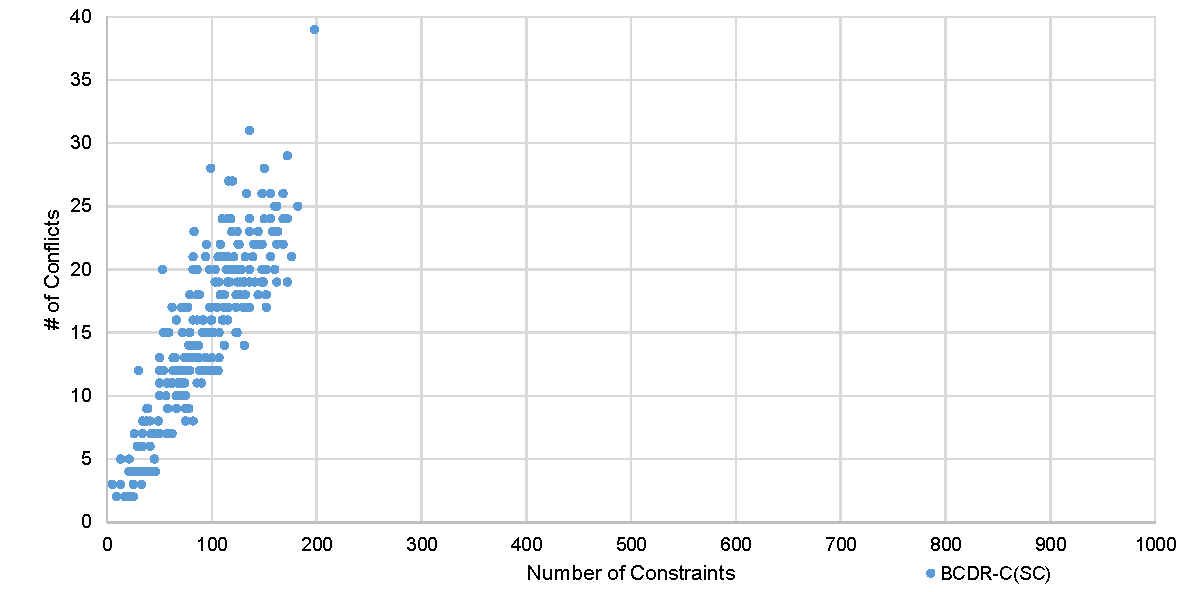
\includegraphics[width=0.9\textwidth]{figures/results/bcdr_cc_sc_conflicts.pdf}
	\caption{Conflicts detected by BCDR-C(SC)}
	\label{fig:bcdrc_sc_conflicts_results}
\end{figure}


\begin{figure}[!ht]
	\centering
	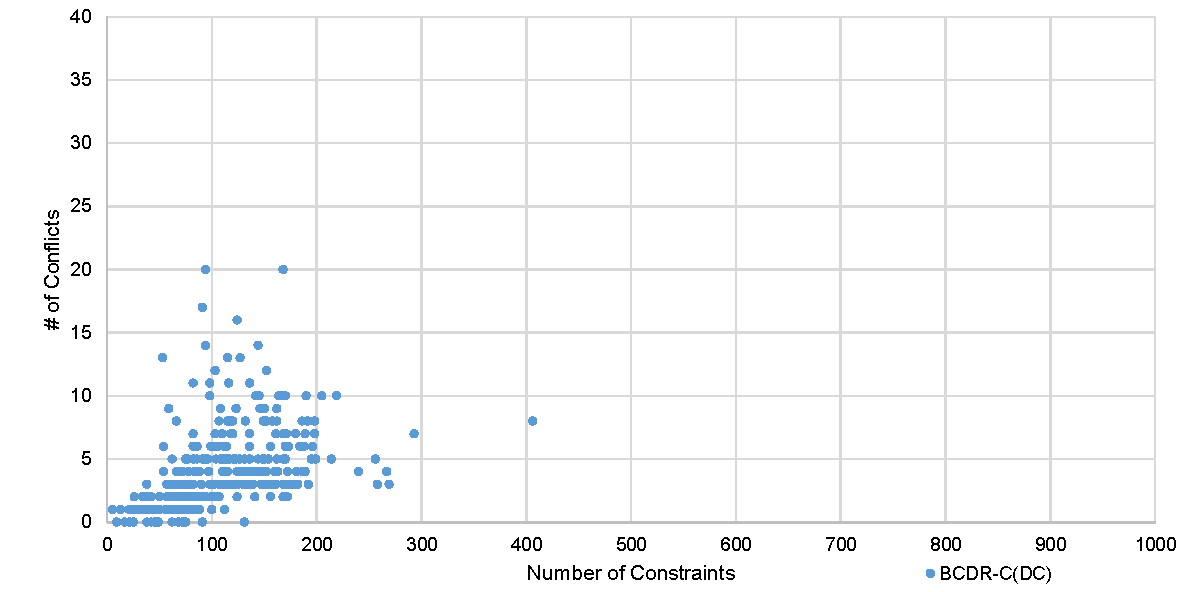
\includegraphics[width=0.9\textwidth]{figures/results/bcdr_cc_dc_conflicts.pdf}
	\caption{Conflicts detected by BCDR-C(DC)}
	\label{fig:bcdrc_dc_conflicts_results}
\end{figure}


BCDR performs much better on problems with set-bounded uncertainty models, since
all constraints are linear during conflict resolution. On the other hand,
non-linear models, such as normal distribution, is better for describing the
uncertainty in some real world activities (e.g. the timing of natural
phenomena). Even though it requires much more computation time, BCDR-C was able
to resolve most of the problems with less than 200 constraints in 30 seconds.
This is enough for modeling a 10-hour survey mission of several underwater
vehicles working in parallel. In general, the algorithm configuration and
modeling should be different from one application to another. The choice of
uncertainty and controllability model to use is thus application dependent. In
addition, results from this experiment also suggest that tractability must be
considered when selecting these models.



\subsection{Optimizing Dispatching Strategies for Maintaining Headways on Transit Routes}


In this section, we discuss a different application of BCDR in the domain of
transit system management. Due to unexpected delay in travel and dwelling,
transit vehicles sometimes cannot operate on schedule and maintain their
designated headways. If a vehicle is delayed and operating off schedule, the gap
between it and an earlier vehicle will increase, causing it to carry more
passengers, spend more time at each station for dwelling and get delayed even
more. In some extreme scenarios, passengers waiting at a station may see two or
more vehicles along the same route arrive together, and find an overcrowded
vehicle followed by near-empty ones. This problem is often called
\textit{bunching} or \textit{platooning} in public transportation, and is a
major challenge for reliable transit service.


This problem has been investigated by many researchers in operation research,
and \citeA{bellei2010transit} presents more details about it. Here we present a
simple example, constructed based on an SBS Transit article on bus
bunching\footnote{`Sometimes, two buses of the same service arrive at the same
time with one bus being overcrowded and the other almost empty. Why?',
\url{http://www.sbstransit.com.sg/doyouknow/facts_bus.aspx.}}, to explain this
problem. Assume that three three vehicles are running in 8-minute intervals and
demand along the route is constant (Figure \ref{fig:bus_bunching1}).


\begin{figure}[htb]
	\centering
	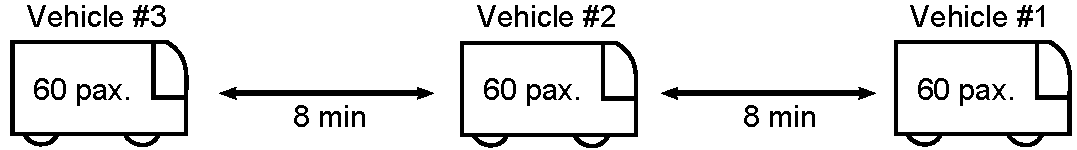
\includegraphics[width=0.7\textwidth]{figures/MBTA/bunching1.pdf}
	\caption{Regular headways between vehicles}
	\label{fig:bus_bunching1}
\end{figure}

Vehicle \#1 and \#3 did not experience any delay in its operation and was able
to keep to schedule. Vehicle \#2 encountered some issues while dwelling at a
previous station. Hence, the headway between Vehicle \#1 and \#2 was lengthened,
while the headway between Vehicle \#2 and \#3 was shortened (Figure \ref{fig:bus_bunching2}).

\begin{figure}[htb]
	\centering
	\includegraphics[width=0.7\textwidth]{figures/MBTA/bunching2.pdf}
	\caption{Uneven headways and passenger load due to delayed Vehicle \#2}
	\label{fig:bus_bunching2}
\end{figure}


By taking more than its share of passengers Vehicle \#2 slowed down as a result,
while Vehicle \#3 picked up fewer passengers.
As this continues, Vehicle \#2 would eventually bunch up with Vehicle \#3. To a
passenger waiting for Vehicle \#2, he would have waited for 6 minutes, and it
would seem that Vehicle \#2 was crowded while Vehicle \#3 was relatively empty.


Current approaches for preventing vehicle bunching heavily rely on the
operators' experience and intuition: they have to respond quickly enough to any
irregular operations before they propagate to the entire route. In addition, the
operators have a very limited set of actions to take, such as asking the delayed
buses to skip stations or urge the passengers to wait for the next bus. Both may
cause inconvenience for passengers either on board or waiting at stations.


Here, we present a dynamic scheduling approach for managing a transit route to address this problem.
Given the schedule of an existing transit route and historical performance data,
we use BCDR to compute a robust dispatching strategy for the vehicles on
this route, such that the headways between buses/trains can be better
maintained. It builds in additional buffer time for vehicles to wait at each
station based on the uncertainty, which allows a dynamically controllable
dispatching strategy to be generated. The dispatching strategy, represented as an
execution policy for events in the scheduling problem, provides real-time
guidance for pausing vehicles at each station in order to maintain headways
along the route. For the passengers, it means that the frequency of services is
more regular, such that they are less likely to wait for an extended period of
time for the service, or board an overly crowded vehicle.


Our approach is similar to the frequency-based method proposed by
\citeA{bartholdi2012self}, which has each bus observe the preceding and
following ones, and strategically delay themselves at stations to maintain
regular headways. As presented in the same paper, this method has been shown to
outperform prior work in controlling the university bus system at Georgia
Institute of Technology. The major difference between it and our scheduling
based approach is that we used a centralized algorithm and pre-compute the
strategy based on historical data. It allows us to coordinate all vehicles along
the route simultaneously, and restore from service interruptions quickly without
waiting for the bus delays to propagate from one to another. However, the
trade-off is that the dynamic policy requires more computation time to
generate, and the policy itself may become invalid if any travel or dwell time
along the route falls outside the set-bounds for uncertain durations.


The objective of this experiment is to explore different problems that
BCDR can solve and benchmark its scalability. The work presented in this section
is not part of any research project, and results have not been compared to other
approaches in the field. We have not verified this approach on any real transit
routes, though we would very much like to share it and evaluate this approach in
a real-world system.


\subsubsection{Setup}


We selected the Red Line subway \footnote{\url{http://www.mbta.com/schedules_and_maps/subway/}} in Boston for this experiment. It is the busiest
mass transit route in the city, carrying more than 250,000 passengers per day.
The agency operating Red Line, the Massachusetts Bay Transit Authority, has been
publishing performance data for every train operation since June 30, 2015. Using
their API, we were able to retrieve the travel times of each train between
stops, and the amount of time the train dwelled at every stop. Combined with the
published schedule, we constructed a CCTPU for modeling the operation of the Red
Line. To simplify the problem, our model covers only the inbound direction
trains from Alewife station to JFK/UMass station (before the line branches into
two directions).


The travel time of each train between stations and dwell times are represented
by uncertain durations, while the scheduled headways are encoded as simple
temporal constraints. Figure \ref{fig:mbta_cctpu_example} is cropped from the
visualization of the problem, which shows a small portion of the CCTPU that
presents all basic elements: dwell, wait for departure, and traversal to the
next station. Given a train ride, the three elements are repeated for each
station pair. The collection of constraints for one train ride are then repeated
for all 167 trains during a peak day along the inbound direction. Between
neighboring trains, the headway constraints are added between their their
arrival events at a station. The temporal bounds of these constraints are
defined using the scheduled headway: [$Headway-1$,$Headway+1$]. We slightly
weakened the headway requirements from the schedule by $\pm$1 minutes to allow
some flexibility for handling uncertainty, such that more efficient solutions
can be generated.


\begin{figure}[htb]
	\centering
	\includegraphics[width=1\textwidth]{figures/MBTA/headway.pdf}
	\caption{Basic elements in the CCTPU for Red Line trains}
	\label{fig:mbta_cctpu_example}
\end{figure}


The bounds for the uncertain durations, travel times, and dwell times are
estimated using the historical performance data: given a train ride between
station A and B, we retrieve train operation data between the same stations in
history and compute a lower and upper bound to cover them. For example, for a
train ride that leaves station Alewife at 5pm, we will retrieve all records for
previous trains that left between 4:30pm to 5:30pm during weekdays, and collect
their travel times between stations and dwell times. For its uncertain duration,
the lower bound is defined using the smallest travel time in the collection,
while the upper bound is chosen such that 98\% of all data points are covered
between the lower and upper bounds.


Given the uncertain durations, there is no execution policy that meets all
constraints in the CCTPU. The objective of this experiment is to restore the
dynamic controllability of the over-constrained CCTPU, by building in the
minimal amount of wait times at each station. We can then compute a dispatching
strategy that is robust against all uncertain travel and dwell times can be
found from the relaxed CCTPU. Therefore, the only relaxable elements in the
CCTPU are the upper bounds of the wait times at each station. The values of the
upper bounds are initialized to be 0.01 minute, and associated with a linear
cost function with gradient 1 to penalize any excessive delays.



\subsubsection{Results}


In this experiment, we solved the over-constrained problems using two
approaches: conflict-directed relaxation with BCDR-U(DC), and a MIP encoding
with Gurobi. For BCDR-U(DC), we use Gurobi as its sub-solver to compute optimal
relaxations for learned conflicts. For the MIP encoding approach, we use Gurobi
directly to solve the complete problem. The MIP encoding we used was first
introduced by \citeA{wah-xin:06} for checking dynamic controllability, and later
a modification was presented by \citeA{cui2015optimising} to evaluate the robustness of schedules for
resource-constrained project scheduling problems. The objective function for
both approaches are set to find the minimum cost relaxations, which correspond
to the minimum delays that have to be built into each station, and makes the
CCTPU for the transit route a dynamically controllable network.


Different from the AUV mission planning problems, the transit operation problem's temporal
network is highly connected due to the headway constraints. They create many
more cycles in the network, which result in more conflicts between constraints.
The larger number of conflicts makes the problems significantly more difficult
to solve. Therefore, given the limited computing resources and experiment time,
we do not expect both approaches to solve the complete problem with 169 trains
and around 10,000 constraints. To benchmark and compare the performance of two
approaches, we generated a set of smaller test problems by capturing only a
subset of the trains and stations. Each of the 48 test problems contains N (2
$\leq$ N $\leq$ 7) trains and M (2 $\leq$ M $\leq$ 9) stops. In this experiment,
we set the timeout of each test run to be 10 minutes.


\begin{table}[htb]
	\centering
	\begin{tabular}{| c | M{1.1cm} | M{1.1cm} | M{1.1cm} | M{1.1cm} | M{1.1cm} | M{1.1cm} | M{1.1cm} | M{1.1cm} |}
		\hline
		7 & 182.62 & x & x & x & x & x & x & x \\
		\hline
		6 & 87.051 & x & x & x & x & x & x & x \\
		\hline
		5 & 27.012 & 314.55 & x & x & x & x & x & x\\
		\hline
		4 & 7.1596 & 120.48 & 370.16 & x & x & x & x & x \\
		\hline
		3 & 1.9395 & 18.362 & 57.251 & 162.20 & 424.35 & x & x & x \\
		\hline
		2 & 0.62508 & 3.2241 & 9.7885 & 19.904 & 51.379 & 80.885 & 200.97 & 346.31 \\
		\hline
		\slashbox{Trains}{Stops} & 2 & 3 & 4 & 5 & 6 & 7 & 8 & 9 \\
		\hline
	\end{tabular}
	\caption{Runtime of BCDR-U with Gurobi as sub-solver (in seconds)}
	\label{table:mbta_bcdr_result}
\end{table}


\begin{table}[htb]
	\centering
	\begin{tabular}{| c | M{1.1cm} | M{1.1cm} | M{1.1cm} | M{1.1cm} | M{1.1cm} | M{1.1cm} | M{1.1cm} | M{1.1cm} |}
		\hline
		7 & 270 & x & x & x & x & x & x & x \\
		\hline
		6 & 160 & x & x & x & x & x & x & x \\
		\hline
		5 & 98.4 & 261 & x & x & x & x & x & x\\
		\hline
		4 & 60 & 202 & 260 & x & x & x & x & x \\
		\hline
		3 & 31.4 & 95 & 130 & 144 & 181 & x & x & x \\
		\hline
		2 & 9.6 & 49 & 75.4 & 82.4 & 112 & 118 & 135 & 154 \\
		\hline
		\slashbox{Trains}{Stops} & 2 & 3 & 4 & 5 & 6 & 7 & 8 & 9 \\
		\hline
	\end{tabular}
	\caption{Number of conflicts resolved by BCDR-U before finding the optimal relaxations}
	\label{table:mbta_bcdr_result_conflicts}
\end{table}


\begin{table}[htb]
	\centering
	\begin{tabular}{| c | M{1.1cm} | M{1.1cm} | M{1.1cm} | M{1.1cm} | M{1.1cm} | M{1.1cm} | M{1.1cm} | M{1.1cm} |}
		\hline
		7 & x & x & x & x & x & x & x & x \\
		\hline
		6 & x & x & x & x & x & x & x & x \\
		\hline
		5 & x & x & x & x & x & x & x & x\\
		\hline
		4 & x & x & x & x & x & x & x & x \\
		\hline
		3 & 30.399 & x & x & x & x & x & x & x \\
		\hline
		2 & 2.7040 & 12.569 & 76.568 & 340.29 & x & x & x & x \\
		\hline
		\slashbox{Trains}{Stops} & 2 & 3 & 4 & 5 & 6 & 7 & 8 & 9 \\
		\hline
	\end{tabular}
	\caption{Runtimes of Gurobi with MIP encoding (in seconds)}
	\label{table:mbta_gurobi_result}
\end{table}



The results are shown in Table \ref{table:mbta_bcdr_result} for BCDR-U(DC), and
Table \ref{table:mbta_gurobi_result} for Gurobi with MIP encoding. Rows indicate the number of trains captured by the test problems, while
columns indicate the number of stops. The run-times of each approach for
solving the test problem are the averaged results from five test runs. Within
the time limit, BCDR-U(DC) solved 20 out of 48 problems with up to 7 trains/2 stops
and 2 trains/9 stops, while Gurobi only solved 5 problems with less than 3
trains and 5 stops. For the problems that both methods solved in the time limit
(2 Trains with 2, 3, 4, and 5 stops, and 3 Trains with 2 stops), BCDR-U(DC) is
roughly one order of magnitude faster than Gurobi with MIP encoding. Similar to
the results from the first experiment, the runtime of BCDR-U(DC) on an
over-constrained problem is largely determined by the number of conflicts in it.
As can be seen in Table \ref{table:mbta_bcdr_result_conflicts}, problems with
more trains and stops generally contain more conflicts, which require longer
runtime for BCDR-U(DC) to solve.


The results demonstrate the advantage of BCDR-U's conflict-directed approach: it
allows the solver to only deal with the conflicts instead of the complete
problem, which significantly reduces the number of constraints and variables it
has to consider. Although BCDR-U's conflict learning step requires a significant
amount of computation, overall the procedure is still worth the effort,
especially for large problems like the transit route optimization. Even for
Gurobi, which is commonly regarded as a state-of-the-art MIP and LP optimizer,
BCDR-U is still able to significantly improve its performance on the relaxation
problems when compared to the direct MIP encoding approach.


\subsection{Robustness Analysis of Resource-constrained Project Schedules}


Finally, we present the application of BCDR to evaluating the robustness of
resource-constrained project schedules. First presented by
\citeA{cui2015optimising}, the objective of
this experiment is very different from the previous two experiments:
instead of over-constrained temporal problems, BCDR is given a feasible problem
and a partial-order schedule for it, and is asked to find the maximum
uncertainty that can be built into the durations of some activities, while
maintaining the controllability of the problem. It is like finding a
configuration of temporal problems that pushes them to the boundary of feasibility.


%Providing flexibility in schedules and temporal plans is viewed as a means to
%increase their robustness against unforeseen disturbances, such as delays.
%Several metrics for the flexibility of a schedule have been proposed
%\cite{cesta-oddi-smith:aips98,aloulou-portmann:03,wilson-etal:aij:14}, as well
%as algorithms for finding high-flexibility schedules
%\cite{aloulou-portmann:03,policella-etal09,banerjee-haslum:icaps11}. However,
%flexibility does not necessarily imply robustness: this depends on how
%'robustness' itself is defined. In abstract terms we may define robustness as
%the greatest level of disturbance (deviation from expected outcomes) at which
%the schedule is still successfully executed. (If we assume a probability
%distribution over deviations is given, the level of disturbance at which the
%schedule breaks equates to the probability of it breaking during execution. We
%consider this case in a later section.) To operationalise this definition, we
%have to specify what kind of disturbances are considered, and how the schedule
%executive can use flexibility to cope with them. Here, we exemplify by assuming
%(1) that the possible disturbances are deviations in the time taken to execute
%an activity from its normal duration, and (2) a partial-order schedule with a
%dynamic execution strategy.


A partial-order schedule (POS) consists of a set of time constraints between
activities such that any realization that meets these constraints is also
resource feasible. In the deterministic case, where the duration of each
activity $i$ is a constant $d_i$, the POS can be represented as an STN with time
points $t_{\taskstarttp{i}}$ and $t_{\taskendtp{i}}$ for the start and end,
respectively, of each activity. Assuming the duration of each activity can vary
within some bounds, $[l_{\taskstarttp{i},\taskendtp{i}},
u_{\taskstarttp{i},\taskendtp{i}}]$, the schedule can be modeled as an STNU
where the link $\link{\taskstarttp{i}}{\taskendtp{i}}$ from each activity's
start to its end is contingent, while remaining time constraints are requirement
links. Thus, given a POS, our measure of robustness is defined as the maximum
deviation (i.e., width of the contingent bound) on any activity at which the
STNU is dynamically controllable.


\subsubsection{Setup}

To compute the maximum deviation allowed in a POS, we will need to slightly
modify the BCDR-U algorithm and problem formulation. First, we initialize the
upper bound of all activity durations to $+\infty$, which is the maximum
possible uncertainty we can build in. It makes the schedule over-constrained,
and allows BCDR-U to start from here to iteratively discover conflicts and restore
the controllability of the schedule. Second, we modify the objective function
used by BCDR-U (Equation \ref{eqn:obj}) to be defined over the range of uncertain
durations (Equation \ref{eqn:max_flex_obj}). Instead of minimizing the costs of
weakening relaxable constraints, this modification allows BCDR-U to maximize the
minimum deviation among all activity durations.


\begin{align}
&\phantom{=}	\max\min_{ub_i'}{(ub_i' - lb_i)};
\label{eqn:max_flex_obj}
\end{align}


Figure \ref{fig:RCPSP_reform} presents a simple example that demonstrates the
modification and the expected output from BCDR-U. Given a feasible schedule over
two activities (Figure \ref{fig:RCPSP_reform1}), we first increase the upper
bounds of the activities to $+\infty$ (Figure \ref{fig:RCPSP_reform2}). The
change effectively applies the maximum possible deviation to the schedule, but
also makes it over-constrained in most scenarios.
Then we apply BCDR-U(DC) on the problem, asking it to extract conflicts introduced by
the modification, resolve them by lowering the upper bound according to the new
objective function, and restore the dynamic controllability of the problem
(Figure \ref{fig:RCPSP_reform3}).


\begin{figure}[h!]
	\centering
	\begin{subfigure}[b]{0.6\textwidth}
		\includegraphics[width=\textwidth]{figures/RCPSP_reformulation/example_cctpu.pdf}
		\caption{}
		\label{fig:RCPSP_reform1}
	\end{subfigure}
	\begin{subfigure}[b]{0.6\textwidth}
		\includegraphics[width=\textwidth]{figures/RCPSP_reformulation/example_cctpu2.pdf}
		\caption{}
		\label{fig:RCPSP_reform2}
	\end{subfigure}
	\begin{subfigure}[b]{0.6\textwidth}
		\includegraphics[width=\textwidth]{figures/RCPSP_reformulation/example_cctpu3.pdf}
		\caption{}
		\label{fig:RCPSP_reform3}
	\end{subfigure}
	\caption{Examples for maximizing flexibility}
	\label{fig:RCPSP_reform}
\end{figure} 



As test cases, we use 325 partial-order schedules for RCPSP/max problems
\cite{kolisch-padman97} with 10--18 jobs\footnote{Set J10 from PSPLIB
(\url{http://www.om-db.wi.tum.de/psplib/})}. The schedules are generated by a
scheduler that optimises a measure of POS flexibility
\cite{banerjee-haslum:icaps11}. The STNU representation of a schedule has a time
point for the start and end of each activity, as described above. Hence, the
number of nodes and contingent links is determined by the number of jobs, but
the number of (given) requirement links varies from 50 to 300.



\subsubsection{Results}


In this experiment, we solved the over-constrained problems using two
approaches: conflict-directed relaxation with BCDR-U(DC), and MIP encoding with
Gurobi. Similar to the second experiment on transit route schedules, we use
Gurobi as the sub-solver for BCDR-U(DC). For the MIP encoding approach, we used the
encoding introduced by \citeA{cui2015optimising} to compute the maximum
flexibility that can be built into the uncertain durations. The problems in this
experiment are of much smaller scale compared to the previous two experiments,
and both approaches were able to solve all problem within the time limit (30
seconds). For each test run, we recorded the computation times of both approaches for comparison.


\begin{figure}[htb]
	\centering
	\includegraphics[width=1.0\textwidth]{figures/results/rcpsp_runtime.pdf}
	\caption{Runtimes of BCDR-U(DC) and Gurobi/MIP on RCPSP schedules (in seconds)}
	\label{fig:rcpsp_results}
\end{figure}


The results are shown in Figure \ref{fig:rcpsp_results}: each data point in the
graph represents the averaged runtime for one problem over five test runs. Similar to
the results from the previous experiments, BCDR-U(DC) is very effective for solving
these problems when compared with the MIP/Gurobi approach, which is about one
order of magnitude slower on most test problems.


\begin{figure}[htb]
	\centering
	\includegraphics[width=1.0\textwidth]{figures/results/rcpsp_candidates.pdf}
	\caption{Numbers of candidates evaluated by BCDR-U(DC) on RCPSP schedule problems}
	\label{fig:rcpsp_candidates}
\end{figure}


Among the 325 test runs, we observed one interesting out-lier in the result:
BCDR-U(DC) spends more time solving Instance 135 than Gurobi. This is the
only case in which BCDR-U(DC) spends more time, and we were interested in
investigating the cause behind this issue. We started with the number of
candidate relaxations evaluated in solving the problem (Figure
\ref{fig:rcpsp_candidates}). Not surprisingly, BCDR-U(DC) tested many more
candidates before reaching the optimal relaxations for Instance 135 (the 825th
candidate dequeued), which explains the longer runtime on this problem. Next, we
retrieved the utility of candidates generated by BCDR-U(DC) while solving
Instance 135. Figure \ref{fig:rcpsp_candidate_utilities} presents the utility
of BCDR-U(DC)'s candidates in a test run: from the first feasible candidate
(Index 1 with utility 7.6667) to the final solution (Index 825 with utility
5.1429). There are a few `plateau' regions in the graph, which indicate that
BCDR-U(DC) spent a lot of time evaluating candidates of similar utility without
making progress towards the solution. This indicates one of the weakness in
BCDR-U(DC)'s best-first enumeration approach: without a good heuristic function
for computing the bounds on continuous relaxation costs, BCDR-U(DC) may waste a
large amount of time exploring parts of the search space it believes to be
promising, but which in fact contain no good solutions. This issue is more often
observed in problems with many conflicts, since each conflict may introduce
multiple continuous relaxations and significantly enlarge the search space.
Therefore, a heuristic function for estimating the bound on relaxation cost
should be incorporated whenever available, and developing a general application
bounding function for continuous relaxation is part of our future research.



%We believe that a better heuristic function that folds in the number of candidates will be helpful: the tie-breaker, such that we can prioritize the evaluation of candidates that have solved more candidates. The evaluating candidates that is not helping to discover new conflicts.


\begin{figure}[htb]
	\centering
	\includegraphics[width=1.0\textwidth]{figures/results/rcpsp_candidate_utility.pdf}
	\caption{Utilities of candidates evaluated by BCDR-U(DC) while solving Instance 135}
	\label{fig:rcpsp_candidate_utilities}
\end{figure}




\section{Conclusion}

In this paper, we presented the Best-first Conflict-Directed Relaxation
algorithm for resolving over-constrained temporal problems. BCDR takes a
conflict-directed approach and leverages prior work on hardware diagnosis,
temporal controllability checking, and chance-constrained scheduling. Compared to
previous approaches, which resolve over-constrained problems by suspending
constraints, BCDR minimizes the perturbation by continuously relaxing temporal
constraints to the minimal extent. With the implementation of an incremental
conflict learning and resolution strategy, the algorithm is efficient at
enumerating relaxations in best-first order, and can incorporate user inputs
during the process. 

In addition, BCDR can be easily extended to handle problems
with temporal uncertainty, either expressed as set-bounded uncertain durations,
or probabilistic durations with chance constraints. The two variants, BCDR-U and
BCDR-C, allow the users to diagnose the source of uncertainty in an
over-constrained temporal problem, and enumerate preferred resolutions with
bounded risk. They help the users to resolve conflicts in temporal problems by
trading off safety margins with performance; providing flexibility for
risk management in real world scenarios. 

BCDR and its extensions have been
incorporated as part of several decision support applications for deep-sea
exploration, transit route management and job-shop schedule robustness analysis.
Results from our experiments in these domains have demonstrated the algorithm's
effectiveness in resolving large and complex problems.


\bibliographystyle{theapa}
\bibliography{jair}

\end{document}
